\documentclass[12pt, a4paper,twoside,parskip=full]{report}
	\usepackage{comment}
	\usepackage{mathtools,amsthm} % Enable useful mathematical symbols/environments
	\usepackage{graphicx} % Enable graphics
	\usepackage{fancyhdr,titlesec,microtype} % enable various formatting commands
	\usepackage[margin=2.5cm]{geometry} % Set margin size
	\usepackage{merriweather} % Set the font
	\usepackage[latin1]{inputenc} % Allow you to input accents, umlauts and other characters
	\usepackage[T1]{fontenc} % Lets LaTeX print a wider array of characters
	\usepackage{tablefootnote}
	\usepackage[most]{tcolorbox}
	\usepackage{xcolor} % Enable coloured elements
	\definecolor{mypurple}{HTML}{622567}
	\definecolor{primaryc}{HTML}{8f5e77}
	\definecolor{myblue}{HTML}{007A87} 
	\usepackage{footnotehyper}
	\usepackage{caption}
	\usepackage{subcaption}
	\usepackage{indentfirst}
	\edef\restoreparindent{\parindent=\the\parindent\relax}
	\usepackage{parskip}
	\restoreparindent
	
	% For technical reasons, hyperref should be loaded after all other packages
	\usepackage[colorlinks,linkcolor=myblue,citecolor=mypurple, urlcolor=myblue]{hyperref}
	
	
	\renewcommand{\baselinestretch}{1.5} % 1.5 line spacing
	
	% Define \begin{theorem}, \end{theorem}, etc.
	\theoremstyle{plain} % The following will be italicised
	\newtheorem{theorem}{Theorem}[chapter]
	\newtheorem{lemma}[theorem]{Lemma}
	\newtheorem{proposition}[theorem]{Proposition}
	\newtheorem{corollary}[theorem]{Corollary}
	
	\theoremstyle{definition} % The following environments will not use italics
	\newtheorem{definition}[theorem]{Definition}
	\newtheorem{example}[theorem]{Example}
	
	\theoremstyle{remark} % The following environments will not use italics or bold titles
	\newtheorem{remark}[theorem]{Remark}
	
	\numberwithin{equation}{chapter}
	
	\addtolength{\skip\footins}{4pc plus 5pt}
	\setlength{\footnotesep}{1.22\footnotesep}
	
	% Fancy headings
	\pagestyle{fancy}
	\setlength{\headheight}{15pt}
	\fancyheadoffset[LE,RO]{0pt}
	\renewcommand{\chaptermark}[1]{\markboth{#1}{}}
	\renewcommand{\sectionmark}[1]{\markright{\thesection\ #1}}
	\fancyhf{}
	\fancyhead[LE]{\makebox[0pt][l]{\thepage}\hfill\leftmark}
	\fancyhead[RO]{\rightmark\hfill\makebox[0pt][r]{\thepage}}
	\fancypagestyle{plain}{%
		\fancyhead{} % get rid of headers
		\renewcommand{\headrulewidth}{0pt} % and the line
	}

	% Fancy  numbers
	\titleformat{\chapter}[display]
	{\normalfont\bfseries\color{primaryc}}
	{\filleft\hspace*{-60pt}%
		\rotatebox[origin=c]{90}{%
			\normalfont\color{black}\Large%
			\textls[180]{\textsc{Section}}%
		}
		\hspace{10pt}%
		{\setlength\fboxsep{0pt}%
			\colorbox{primaryc}{\parbox[c][3cm][c]{2.5cm}{%
					\centering\color{white}\fontsize{80}{90}\selectfont\thechapter}%
			}
		}
	}
	{10pt}
	{\titlerule[2.5pt]\vskip3pt\titlerule\vskip4pt\LARGE\sffamily}
	
	\begin{document}
		
		
		\thispagestyle{empty} % For the title page, no header / footer
		
		\noindent
		\begin{minipage}{0.1\textwidth}
		\end{minipage}
		\hfill
		
		\begin{center}
			\noindent\textcolor{primaryc}{\rule{\linewidth}{4.8pt}}
			
			\vspace{2em}
			
			\vspace{3em}
			\noindent {\Huge{\color{myblue} Claims Denials In U.S. Health Insurance}}
			
			\vspace{3em}
			\noindent {\small \bf Mike Gartner}
			
			{\small \today }
			\vfill
			Claims denials in U.S. health insurance pose a serious problem for patients navigating their care. In this report we present and analyze data that sheds light on the occurrence and prevalence of claims denials, propose policies to improve patient outcomes, and highlight existing avenues for consumer recourse. Our analyses show that claims denials correspond to a highly valuable population
			of claims, and that even modest improvements to appeal access and outcomes
			have the potential to return billions of dollars to consumers.
			\vfill
			

			
			\vspace{0.5em}
			\noindent\textcolor{primaryc}{\rule{\linewidth}{4.8pt}}
			

			
			\vspace{3em}
			
\includegraphics[width = 10mm]{images/persius/favicon.png}
			\hspace{2mm}
			
\includegraphics[width = 50mm]{images/persius/persius_f1_maroon.png}\\[8ex]
		\end{center}
		
		\clearpage
		
		%%%%%%%%%%%% END TITLE PAGE %%%%%%%%%%%%
		
		\tableofcontents
		
		% If you have lots of figures with captions / numbers, uncomment the following line
		%\listoffigures
		
		% If you have lots of tables and want a list of them, uncomment the following line
		%\listoftables
		
		\chapter{Introduction}\label{intro}
		
		Claims are a fundamental and atomic unit of U.S. health insurance: every time an insured consumer attempts to use their health insurance to cover a portion of a bill, a claim is submitted to their insurer on their behalf. The claim records details about the care received and its cost necessary for an insurer to make a payment determination. The primary role of health insurers is to receive and adjudicate these claims based on the contracts they sell, and ultimately pay for some portion of them, on behalf of those who purchased the contracts (typically employers or individuals).
		
		When insurers adjudicate a claim to determine whether they will pay for it, they review the contracts that govern the coverage which has been purchased on behalf of the insured. The permissible content in these contracts is often restricted by various laws and regulations, and the contracts may also refer to external sources (e.g. ``clinical policy bulletins'', or ``scientific literature'') that are explicitly cited as things that will be used to inform coverage determinations. We will say a coverage decision or denial is contractually inappropriate if the decision is inconsistent with the insurance contract governing a policy, or the laws and regulations that apply to that policy.
		
		We note that there are many coverage decisions that one might deem morally or medically inappropriate that would not be considered contractually inappropriate. For example, it would be morally troubling for corporations to sell policies that opaquely exclude the coverage of commonly used, scientifically proven, but expensive treatments for those facing dire medical situations, and then to enforce those exclusions no matter the extenuating or dire circumstances. However, such behavior is, unfortunately, not necessarily contractually inappropriate or illegal, depending on the contract in question.
		
		The prevalence of contractually inappropriate claims denials, and lack of recourse for consumers even in these cases, have been serious problems for a long time. There are organizations that regularly publish reports analyzing the limited publicly available claims denial data \cite{pollitz2021} that point to this prevalence (e.g. when comparing appeal rates to appeal overturn rates), and the subject has been discussed in policy research, legal research \cite{fox2022} and popular journalism \cite{konrad2010} for a long time.
		
		Recently, there have been numerous investigations and articles that have brought to light for the general public just how damaging some of the inappropriate practices taking place really are \cite{armstrong2023a} \cite{armstrong2023b}, and illuminated the scarcity of publicly available data \cite{fields2023}. Finally, there are those most seriously affected; many patients with dire, serious, or chronic medical needs (and their friends and families) have long known about the lack of recourse they enjoy, and the frequency with which contractually inappropriate denials occur just in seeking their own care -- they have been on the front lines for decades, suffering the consequences of an inadequately regulated industry.
		
		In this work, we set out to illuminate the extent and prevalence of claims denials,
		and the crucial monetary role they play in our systems. To do so, we analyze publicly
		available claims denial and appeal data, in more depth than such data has previously been
		studied. We seek to do this analysis in a careful, transparent,
		and reproducible way, to ensure that our work can be extended and used by others
		seeking to improve patient outcomes, justice, and accountability. We discuss this more
		explicitly in the \hyperref[reproducibilitystatement]{transparency statement} below. It is our hope
		that the analyses in this report can be used to catalyze change, such as in supporting those
		seeking to convince decision makers to enact relevant policy.
		
		\chapter{Transparency Statement}\label{reproducibilitystatement}
		
		We aim to publish reports in such a way that all of our analyses, plots,
		and numerical claims drawn from data can be vetted, reproduced, and built upon as desired.
		We believe the ability to reproduce results \emph{end to end} is crucially relevant in discussions
		of this topic, as existing data and transparency are scarce and poorly understood, and there are
		many conflicting voices and viewpoints in the space.
		
		
		To this end, we provide transparent, open source access to all analyses and data used to
		generate this document. The interested reader may probe \emph{any} aspect of our end to end 
		analyses of raw data provided by government institutions by investigating the following resources:
		
		\begin{itemize}
			\item All figures appearing in this report were
			generated via the code housed
			\href{https://github.com/TPAFS/investigations/tree/initial_denial_investigation/investigations/claims_denials}{here}.
			
			\item Data we obtained via public records, not available elsewhere on the internet at the time of writing, is hosted \href{https://github.com/TPAFS/public-records}{here}.
			
			\item A \emph{static} copy of this entire article, including the source used to generate it,
			is housed \href{https://github.com/TPAFS/investigations/tree/main/investigations/claims_denials/latex}{here}.
			
		\end{itemize}
		
		If you believe there are errors in this report, analytical or otherwise, we want to hear about it.
		Feel free to \href{https://github.com/TPAFS/investigations/issues}{open an issue}
		in our public analyses, or send us a message at \href{info@persius.org}{info@persius.org}.
		
		The entire purpose of being completely transparent about our end to end processes is to achieve rigorous 
		results that can be audited by anyone, and that constitute trustworthy evidence that improves in quality over
		time.  We hope to build trust with you, our readers,
		by being explicitly cognizant of the fact that we are liable to make analysis mistakes, and empowering and imploring
		you to shine a light on any such mistakes, for our collective benefit. We thank you for your support in this effort.
	
		
		\chapter{A Primer On Claims Denials}\label{primer}
		
		A \emph{claim denial} occurs when a claim is submitted to an insurer, and the insurer decides they will not pay for it. In practice, such decisions are made for many reasons; some valid \footnote{\emph{Valid} here could mean medically, morally or contractually valid. We again note that these notions of validity are rarely the same. We will always explicitly qualify the words appropriate or valid if we are specifically referring to a particular notion.}, and others inappropriate or indefensible.
		
		When a claim is denied, a patient is typically left with an out of pocket expense larger than what they would otherwise face.

		\subsection{Denials}
		
		One of the most basic metrics that one can use to investigate how claims handling varies is an overall \emph{claims denial rate}. This measures the fraction all claims submitted that are denied:
		
		\begin{equation*}
			\text{Denial Rate} = \dfrac{\text{Claims Denied}}{\text{Claims Received}}
		\end{equation*}
		\hfill\\
		In fact, this is not a uniquely defined notion, because the numerator and denominator can be defined in various ways. For example, one could compute this ratio for all claims submitted to a particular insurer over the course of a year, or for all of the claims submitted for a particular plan over a month, or even for all claims submitted from just one individual to a given plan over the course of a year \footnote{Trying to estimate this last number when choosing an insurer is particularly important for individuals with serious health needs who would be unable to afford the care they need if it were to get denied by their insurer.}. We will calculate denial rates that fit this form from a few different lenses in what follows.
		
		It is worth noting that:
		
		\begin{enumerate}
			\item \emph{Among the claims that are appropriate}, low denial rate is always a good thing for patients. \footnote{Of course not all claims are actually appropriate. For example, sometimes two duplicate claims are submitted for the same care (administratively inappropriate), and approving such claims would in no way help patients. }.
			\item High denial rates can be caused by numerous things, and do not always indicate \emph{contractually inappropriate} insurer practices.
		\end{enumerate}
		
		
		\subsection{Appeals}
		
		When insurers deny claims, patients are often entitled to an appeals process (e.g. those with federal marketplace plans \href{https://www.healthcare.gov/appeal-insurance-company-decision/appeals/}{are afforded such recourse}, as are all others with so-called \emph{non-grandfathered} qualified health plans; see \cite{pollitz2021} for more background).
		
		The details of these processes vary based on details of ones insurance plan, but typically they allow patients to initially file an internal appeal of the denial, which is adjudicated by the insurer themselves. If the internal appeal process (which in some plans requires two attempts at an internal appeal) results in the insurer upholding their denial, patients are then often able to file an external appeal. This means they can submit an appeal of the decision to a (purportedly unbiased \footnote{While we do not have evidence to suggest these organizations make determinations in ways biased towards favorable insurer outcomes, we maintain a healthy dose of skepticism about the independence of their decisions, given the landscape of perverse incentives plaguing the entire space. For example, it is unclear to what extent employees migrate between insurance companies and external review agencies. We invite regulators and lawmakers to publish more data publicly supporting the independence and unbiased nature of such agencies. Lack of public consumer access to detailed denial data, including e.g. determination patterns and methodologies among different review agencies, inspires distrust in a system alread plagued by injustices.}) third party, who is responsible for weighing on the decision; insurers are then legally obligated to uphold the final determinations of these third parties. The third parties, and processes by which external appeals are submitted to them and reviewed by them, vary by plan and by state.
		
		In understanding the landscape of claims denials, it is useful to understand the frequency of occurrence, and distribution of outcomes, of these appeal processes.
		
		\subsubsection{Initial Appeal Rates}
		
		We define the \emph{internal appeal rate} to be the fraction of denied claims that are appealed at the lowest level available to consumers.
		
		\begin{equation*}
			\text{Internal Appeal Rate} = \dfrac{\text{Claims Appealed (@ first level)}}{\text{Claims Denied}}
		\end{equation*}
		\hfill\\
		
		Again, this is a loose definition that we will specify more precisely in each particular calculation below.
		
		Of those denials that are internally appealed, we denote the fraction that are overturned by the insurer as the \emph{internal appeal overturn rate}.
		
		\begin{equation*}
			\text{Internal Appeal Overturn Rate} = \dfrac{\text{Claims Overturned (@ first level)}}{\text{Claims Appealed (@ first level)}}
		\end{equation*}
		\hfill\\
		
		
		\subsubsection{External Appeal Rates}
		
		We define the \emph{external appeal rate} to be the fraction of internally appealed and subsequently upheld denials which are then additionally externally appealed by consumers.
		
		\begin{equation*}
			\text{External Appeal Rate} = \dfrac{\text{Claims Appealed Externally}}{\text{Claims Internally Appealed and Upheld}}
		\end{equation*}
		\hfill\\
		
		
		Of those denials that are externally appealed, we denote the fraction that are overturned by a third party as the \emph{external appeal success rate}.
		
		\begin{equation*}
			\text{External Appeal Success Rate} = \dfrac{\text{Claims Overturned Externally}}{\text{Claims Appealed Externally}}
		\end{equation*}
		\hfill\\
		
		
		\subsubsection{Expected Appeal Phenomenology}
		
		We expect initial appeal success rates to be lower than external appeal success rates, assuming the same population of claims were reviewed \footnote{Note that in practice, one can't compare external and internal appeal success rates directly for the same pool of claims denials. Those appeals that make it to an external review have typically already been through an internal review that was upheld, so the distribution of externally reviewed claims almost never includes e.g. denial cases that an insurer agrees are contractually inappropriate. Presumably, all such cases where an insurer agrees to overturn their initial decision would also be overturned by third parties, if the third parties ever saw them.}. We hold this expectation for two reasons. One is that insurers have a monetary incentive to uphold denials, while third parties do not. The other is that insurers make the initial determinations about what claims to deny, so they obviously have some alignment with the initial denial rationale to begin with. On the other hand, external reviewers may view claims from completely different lenses than that with which an insurer initially viewed them, leading to a higher likelihood of a different conclusion about contractual validity.
		
		Finally, we note that both the internal and external appeal systems have the potential to be completely biased, so we should take care to note when we are drawing conclusions from the data that assumes some impartiality in either process. We expect that of all of the data publicly available, external appeal success rates can best inform the underlying validity of (some subset of) initial denials, since at least one third party with no monetary stake in the judgment has been involved in adjudication. Internal appeal data reflects a situation that presents serious risk for bias by virtue of its design -- it is difficult to take seriously the purported impartiality of a reviewer that is both reviewing their own decision, and that stands to generate more profit by upholding that decision. There is a reason we don't have juries consisting of the best friends of a defendant.
		
		\chapter{Public Claims Denial Data}\label{publicdata}
				
		\subsection{Overview}\label{publicdata:overview}
		To understand the landscape of claims denials, contractually inappropriate claims denials, appeals, and effective consumer recourse, we need data. Unfortunately for consumers, requirements for insurers to publicly disclose claims denial data are few and far between, and the extent to which requirements that do exist are enforced and regulated is unclear. It would be invaluable for regulators to require broad, transparent claims denial information, and to strictly enforce and audit validity of the data.
		\subsection{Datasets}\label{publicdata:datasets}
		
		\begin{itemize}
			\item Federal Marketplace Public Use Files \href{https://www.cms.gov/cciio/resources/data-resources/marketplace-puf}{Public Use Files}(PUFs) from the Centers for Medicare and Medicaid Services (CMS)\\
			
			\begin{tcolorbox}[enhanced, breakable]
			Each year CMS releases a collection of transparency data related to federal marketplace insurers. Here we are interested in the \emph{transparency in coverage}  \begin{comment}\footnote{The term transparency in coverage has been overloaded, and used in different contexts by CMS and other government agencies. Our use of the term here does not refer to the \href{https://www.federalregister.gov/documents/2019/11/27/2019-25011/transparency-in-coverage}{CMS rule published in 2019} requiring health plans to publish certain rate data, which is \href{https://www.cms.gov/healthplan-price-transparency}{broadly being referenced} as the transparency in coverage rule. Instead, it refers only to the \href{https://www.cms.gov/cciio/resources/data-resources/marketplace-puf}{public use files distributed by CMS} documenting federal marketplace denials and appeals (among other things). Note that these are also referred to by CMS as transparency in coverage files, and in fact have been in existence, and referred to in this way, far longer than the TiC rule. Obviously the two efforts are not completely unrelated, and it would be most welcome if reporting requirements in the TiC rule were expanded to incorporate reporting about denial transparency, as do these federal marketplace PUFs. See further discussion in the policy section.}
			\end{comment}
			(TIC) public use files. These are files compiled from self-reported insurer data specifying aggregate counts of claims submitted, claims denied, and claims appealed, among other things. This data is limited in scope, and clearly accuracy is not strictly validated based on the frequency of impossible records in the data, but it is the closest thing we have to a denial transparency requirement with broad impact. It is compiled and reported to the public in accordance with the Department of Health and Human Services (HHS) \href{https://www.ecfr.gov/current/title-45/subtitle-A/subchapter-B/part-155/subpart-K/section-155.1040}{rule 45 of the Code of Federal Regulations (CFR), part 155, subpart K} (cf \href{https://www.ecfr.gov/current/title-45/subtitle-A/subchapter-B/part-156/subpart-C/section-156.220}{CFR 156 subpart C)}.
			
			In this article we focus on the 2023 public use file, which details claims denial data from the 2021 plan year.
			
			This 2021 data corresponds to:
			
			\begin{itemize}
				\item Plan year 2021.
				\item 33 states.
				\item 230 unique insurers.
				\item 6,764 plans.
				\item 8,251,703 consumers.
			\end{itemize}
		
			\end{tcolorbox}
			\item \href{https://www.dfs.ny.gov/reports_and_publications/health_care_claim_reports}{New York Health Care Claim Reports}\\
			
			\begin{tcolorbox}[enhanced, breakable]
			Thanks to \href{https://www.nysenate.gov/legislation/laws/ISC/345}{legislation from 2020}, New York publishes \href{https://www.dfs.ny.gov/reports_and_publications/health_care_claim_reports}{health care claim reports} for insurance companies that contain aggregate counts of claims submitted, claims denied, and claims appealed for each NY insurer, among other things. 
			
			This data, released quarterly as of 2022 in the form of spreadsheets for each New York insurer, details aspects of health insurance coverage for insurance plans in New York. Various details about how the data is reported are included in the frequently asked questions for the data on the \href{https://www.dfs.ny.gov/apps_and_licensing/health_care_claim_reports}{DFS homepage}. 
			
			Residents of New York state can not buy individual Affordable Care Act (ACA) compliant Qualified Health Plans (QHPs) on the federal marketplace. Instead, NY maintains its own marketplace where such plans can be purchased, known as \href{https://nystateofhealth.ny.gov/}{New York State of Health}. The New York Health Care Claims Reports includes statistics relating to NY marketplace plans, in addition to plans that are not sold via the marketplace. 
			
			Unfortunately, the New York state marketplace does not release detailed claims denial and appeal data in the same way such data is reported in the CMS TIC PUFs for federal marketplace QHPs, so we cannot directly reuse the same analyses across the CMS PUF data and the NY Health Care Claims Reports.
			
			We note that we do not consider in this article historical appeals data (including data predating the existence of the health care claims reports) collected and distributed by New York Department of Financial Services in \href{https://www.dfs.ny.gov/system/files/documents/2022/08/ny_consumer_guide_health_insurers_2022.pdf}{consumer reports}; unfortunately, that data does not include raw numbers describing the total population of claims or denials to which the reported appeals pertain, so it is difficult to determine highly relevant context for the appeals numbers.
			
			In this article, we analyze the health care claims report data from 2022. The 2022 data includes:
			
			\begin{itemize}
				\item Plan year 2022.
				\item 29 unique insurers.
				\item 145,446,802 claims adjudicated, worth at least \$66,810,881,848.
				\item 25,996,601 claims denied, worth at least \$2,265,844,512.
				\item 177,917 claims denied for medical necessity, worth at least \$35,747,594.
				\item 145,129 internal appeals adjudicated, worth at least \$303,942,639.
				\item  42,375 overturned internal appeals, worth at least \$124,245,612.
			\end{itemize}
		
			All denials recorded in the data are post-service claims denials, so pre-authorization denials are not included. Appeals in the data include both appeals submitted directly by consumers, and appeals submitted by providers on behalf of consumers.
			\end{tcolorbox}
		
			\item \href{https://www.dfs.ny.gov/public-appeal/search}{New York External Appeal Outcome Data}\\
			
			\begin{tcolorbox}[enhanced, breakable]
			External appeals of denials from New York marketplace plans, fully insured group plans, and Medicaid managed care plans are adjudicated by Independent Review Organizations. The New York Department of Financial Services manages such appeal processes, and maintains a public database of results from external appeals.
			
			The \href{https://www.dfs.ny.gov/public-appeal/search}{New York External Appeal Outcome Data} corresponds to:
			
			\begin{itemize}
				\item Plan years 2019 to 2023.
				\item 24,728 external appeals.
				\item Individual and group health plans.
				\item Fully insured employer plans.
				\item IMRs associated with plans regulated by the New York State Department of Financial Services.
				
			\end{itemize}
		
			In this article we discard the subset of the dataset corresponding to claims from 2023; such claims correspond to an incomplete plan year, and they have the potential to introduce confounding inconsistencies into our analyses. We initially included them in our analyses, but found they led to easily misinterpreted results.
		
			\end{tcolorbox}
			
			\item \href{https://fortress.wa.gov/oic/consumertoolkit/Search.aspx?searchtype=indrev}{Washington External Appeal Outcome Data}\\
			
			\begin{tcolorbox}[enhanced, breakable]
				
			In Washington state, claims denial data is not generally made public. However, as in New York, the final adjudication status of claims which are both ultimately externally appealed and fall under the authority of the Office of the Insurance Commissioner (OIC) are recorded in a \href{https://fortress.wa.gov/oic/consumertoolkit/Search.aspx?searchtype=indrev}{publicly accessible dataset}.
			
			External appeals of denials from Washington marketplace plans are adjudicated by Independent Review Organizations. According to \href{https://apps.leg.wa.gov/wac/default.aspx?cite=284-43-3030}{Washington Administrative Code 284-43-3030} and the \href{https://app.leg.wa.gov/RCW/default.aspx?cite=48.43.530}{Revised Code of Washington 48.43.530}, insurers must support both internal and external appeal processes, and report resulting data to the insurance commissioner. The code above provides for external appeals to be sought as soon as an internal process is exhausted, or 30 days after internal appeal initiation has occurred, whichever is sooner. Details of the rules pertaining to external appeals are described in the \href{https://app.leg.wa.gov/rcw/default.aspx?cite=48.43.535}{Revised Code of Washington 48.43.535}.
			
			The OIC in Washington state maintains the aforementioned public database of results from these external appeals. This data corresponds to consumers enrolled in Washington health plans that are regulated by the Office of the Insurance Commissioner (OIC). This includes, but is not limited to, individual plans sold on the \href{https://wahealthplanfinder.org/}{Washington marketplace} (known as \emph{Washington Health Plan Finder}).
			
			The OIC external appeal database corresponds to:
			
			\begin{itemize}
				\item Plan years 2016 through 2023.
				\item 8,774 external appeals.
				\item Individual and group health plans.
				\item Self insured and fully insured employer plans.
				\item IMRs associated with plans regulated by the OIC.
			\end{itemize}
			
			In this article we discard the subset of the dataset corresponding to claims from 2023; such claims correspond to an incomplete plan year, and they have the potential to introduce confounding inconsistencies into our analyses. We initially included them in our analyses, but found they led to easily misinterpreted results.
			\end{tcolorbox}
			
			\item California External Appeal Data from the \href{https://interactive.web.insurance.ca.gov/apex_extprd/f?p=192:1:2660782937251:::::}{California Department of Insurance (CDI)} and the \href{https://dmhc.ca.gov/AbouttheDMHC/DMHCReports/AnnualReports.aspx}{Department of Managed Health Care (DMHC)}\\
			
			\begin{tcolorbox}[enhanced, breakable]
			
			California releases data related to internal and external appeal outcomes in at least four places, all of which we consider:
			
			\begin{enumerate}
				\item Yearly CDI \href{https://www.insurance.ca.gov/0400-news/0200-studies-reports/0700-commissioner-report/}{commissioner reports}.\\
				
				These reports include summary statistics, such as the total numbers of claims and internal appeals submitted by consumers. The specific yearly reports we consider here are released by commissioner Ricardo Lara. 
				
				\item Yearly DMHC \href{https://dmhc.ca.gov/AbouttheDMHC/DMHCReports/AnnualReports.aspx}{secretary reports}.\\
				
				These reports include summary statistics, such as the total numbers of claims and internal appeals submitted by consumers. The specific yearly reports we consider here are released by director Mary Watanabe.
				
				\item A \href{https://interactive.web.insurance.ca.gov/apex_extprd/f?p=192:1:5191948876739:::::}{database of Internal Medical Review (IMR) outcomes adjudicated by the California Department of Insurance}.\\
			
				This data corresponds to plans regulated by the CDI.
				
				\item A \href{https://data.chhs.ca.gov/dataset/independent-medical-review-imr-determinations-trend}{database of Internal Medical Review (IMR) outcomes pertaining to health maintenance organizations (HMOs)}.\\
				
				This data corresponds to plans regulated by the California Department of Managed Health Care (DMHC).
				
			\end{enumerate}
			
			External appeals in California, also known as Independent Medical Reviews (IMRs), follow processes dictated by two pieces of the California Insurance Code (CIC).
			
			\begin{itemize}
				
				
				\item \href{https://leginfo.legislature.ca.gov/faces/codes_displayText.xhtml?lawCode=INS&division=2.&title=&part=2.&chapter=1.&article=3.5.}{Sections 10169.1 - 10169.5}, which initially became effective January 1, 2001, describe rules that apply to IMR sought for health coverage decisions purportedly related to medical necessity. There have been numerous modifications to the law since then. The current law expressly provides for the inclusion of those on Medicare and Medicare Advantage plans, however it also allows for processes to be subsumed by existing state Medicare resolution outlets. It allows IMRs to be sought as soon as an internal process is exhausted, or 30 days after internal initiation has occurred, whichever is sooner. It also allows the CDI to contract with the DMHC to administer the IMR as desired (which has come into play for managed care plans, such as HMOs, as described in the last dataset description above.)\\
				
				\item \href{https://leginfo.legislature.ca.gov/faces/codes_displaySection.xhtml?lawCode=INS&sectionNum=10145.3.}{Section 10145.3}, also effective as of January 1, 2001, describes particular rules that apply to IMR sought for insurer decisions stemming from deeming treatment or services as experimental or investigational in nature.\\
				
			\end{itemize}
		
			The CDI IMR database corresponds to:
			
			\begin{itemize}
				\item Plan years 2011 through 2023.
				\item 4,719 Independent Medical Reviews.
				\item Individual and group health plans.
				\item Self insured and fully insured employer plans.
				\item IMRs associated with plans regulated by the California Department of Insurance.
			\end{itemize}
			
			The DMHC IMR database corresponds to:
		
			\begin{itemize}
				\item Plan years 2001 through 2023.
				\item 34,615 Independent Medical Reviews..
				\item Individual and group health plans.
				\item Self insured and fully insured employer plans.
				\item IMRs associated with plans regulated by the California Department of Managed Healthcare.
			\end{itemize}
			
			In this article we discard the subset of both datasets corresponding to claims from 2023; such claims correspond to an incomplete plan year, and they have the potential to introduce confounding inconsistencies into our analyses. We initially included them in our analyses, but found they led to easily misinterpreted results.
		
			\end{tcolorbox}
			
			
			\item Connecticut Denial Data From \href{https://portal.ct.gov/CID/Reports/Consumer-Report-Card-on-Health-Insurance-Carriers-in-Connecticut}{Consumer Report Cards}
			
			\begin{tcolorbox}[enhanced, breakable]
			
			Each year Connecticut's Department of Insurance releases a report, the so called \emph{Consumer Report Card on Health Insurance Carriers}. The report includes various aggregate statistics about health insurance plans, including utilization for certain services, member satisfaction, and aggregate denial statistics.
			
			The yearly data is released as a published PDF report, and corresponds to all insurance plans sold by Connecticut issuers except those that are government sponsored; in other words, all CT health insurance enrollees other than those with government sponsored plans (e.g. Medicaid and Medicare plans) are represented. As such, the data pertains to both individual and group health insurance plans, including self insured and fully insured employer plans.
			
			In this article we focus on the 2022 report, which details claims from the 2021 plan year.
			
			The data corresponds to coverage for:
			
			\begin{itemize}
				\item Plan year 2021.
				\item 11 unique insurers.
				\item 1,991,903 consumers.
				\item HMO and indemnity plans.
				\item Individual, small group and large group plans.
				\item Self insured and fully insured plans.
			\end{itemize}
			
			\end{tcolorbox}
		
			\item Pennsylvania Department of Insurance \href{https://repos.persius.org/public-records/data/claims_denials/pa/readme.html}{claims denial data}
			
			\begin{tcolorbox}[enhanced, breakable]
			Pennsylvania utilized the federal marketplace for qualified health plans until the end of 2020, when it transitioned to using its own newly formed marketplace, known as \href{https://pennie.com/}{Pennie}, in accordance with the passage of \href{https://www.legis.state.pa.us/cfdocs/billinfo/billinfo.cfm?syear=2019&sind=0&body=H&type=B&bn=3}{PA House Bill 3}. Beginning in 2021, consumers could buy qualified health plans on the Pennsylvania marketplace.
			
			We submitted a public records request under the Pennsylvania \href{https://www.insurance.pa.gov/right-to-know-law/Pages/default.aspx}{Right to Know Law} to the \href{https://www.insurance.pa.gov/Pages/default.aspx}{Pennsylvania Insurance Department} (PA DOI) asking for a comprehensive account of various aggregate statistics pertaining to claims adjudication for which we believed they were likely to have records. This dataset is the result of that request. While the data is not as comprehensive or extensive as we had hoped might be possible, it is a step forward. We are releasing the raw data we obtained, as well as parsed and preprocessed adaptations of it, to the public along with the release of this article.
			
			The dataset contains aggregate counts for claims, denials, and internal and external appeals broken down by issuer for claims corresponding to marketplace plans, plus an undisclosed additional population of plans, from plan years 2020 and 2021. In addition, the data includes claims, denials and denial rationales broken down by \emph{plan} for the subset of claims corresponding specifically to marketplace plans (this subset constitutes a large majority of the dataset to begin with).
			
			The data obtained from the PA Department of Insurance corresponds to:
			
			\begin{itemize}
				\item Plan years 2020 and 2021.
				\item 13 unique insurers.
				\item 599 unique plans.
				\item At least 337,722 consumers.
				\item 21,646,696 claims adjudicated.
				\item 2,964,421 claims denials.
				\item 2,751 internal appeals.
				\item 103 external appeals.
				\item Individual marketplace plans.
				\item \emph{Possibly} additional group plans regulated by the PA Department of Insurance.
			\end{itemize}
		\end{tcolorbox}
	
	
	
		\end{itemize}
	
		
		To our knowledge, this is the first report that compiles aggregate results across a wide array of disparate sources containing claims denial data from different market segments, and the first public report to analyze claims denial data from the Pennsylvania marketplace.
		
		An overview of the data we analyze in this report is detailed in Tables \ref{summarytable1} and \ref{summarytable2} below.
		
		
		\begin{table}[!ht]
			\centering
			\begin{tabular}{|p{3cm}|p{4cm}|p{2cm}|p{3cm}|p{3cm}|}
				\hline
				\textbf{Data Source} & \textbf{Market Segment} & \textbf{Number \newline of \newline Denials} & \textbf{Denial  Levels Represented} & \textbf{Consumer Population  Represented}  \\ \hline
				CMS TIC PUF (2021) & Federal marketplace & 48,302,001 & All & 8,251,703 \\ \hline
				NY Health Care Claims Reports (2022) & All NY Issuers & 25,996,601 & All & Unknown, but $\geq$ 5,000,000 \tablefootnote{ We planned to estimate this population using the \href{https://www.dfs.ny.gov/system/files/documents/2022/08/ny_consumer_guide_health_insurers_2022.pdf}{DFS consumer report for the 2021 plan year}, but found it does not include enrollment. However, we can say that the population of consumers corresponding to plans that the DFS regulates at least includes marketplace plans, and according to New York State of Health \href{https://info.nystateofhealth.ny.gov/enrollmentdata}{enrollment data}, that population has hovered between 4.5-7 million over the years represented here.}  \\ \hline
				NY External Appeals Database (2019-2023) & NY marketplace, fully insured group plans, and Medicaid managed care plans & 26,036 & Externally Appealed (IMR) & Unknown, but $\geq$ 5,000,000  \\ \hline
				WA External Appeals Database (2016-2023) & WA marketplace & 8774 & Externally Appealed (IMR) & 222,731  \\ \hline
			\end{tabular}
			\caption{Summary of Datasets Considered (1/2)}
			\label{summarytable1}
			\end{table}
			\clearpage
		
			\begin{table}
		
		
			\begin{tabular}{|p{3cm}|p{4cm}|p{2cm}|p{3cm}|p{3cm}|}
				\hline
				\textbf{Data Source} & \textbf{Market Segment} & \textbf{Number \newline of \newline Denials} & \textbf{Denial  Levels Represented} & \textbf{Consumer Population  Represented}  \\ \hline
				CA DOI External Appeals Database (2011-2023) & CA marketplace, and fully insured group plans & 4,658 & Externally Appealed (IMR) & 852,506 \tablefootnote{We use the total enrollment noted in the \href{https://www.insurance.ca.gov/0400-news/0200-studies-reports/0700-commissioner-report/}{2021 CDI report}, since it is explicitly noted. This number is therefore relevant for the subset of the database containing IMRs from 2021, but not other years, since the consumer population in this market segment changes yearly. }  \\ \hline
				CA DMHC External Appeals Database (2001-2023) & Large group and self funded plans regulated by DMHC & 34,615 & Externally Appealed (IMR) & 23,474,332 \tablefootnote{We use the total enrollment noted in the \href{https://dmhc.ca.gov/AbouttheDMHC/DMHCReports/AnnualReports.aspx}{2021 DMHC secretary report}, since it is explicitly noted. This number is therefore relevant for the subset of the database containing IMRs from 2021, but not other years, since the consumer population in this market segment changes yearly.}  \\ \hline
				Connecticut Consumer Report Card (2021) & All CT issuers (excluding government sponsored) & 2,708,724 & All & 1,991,903 \tablefootnote{We use the total enrollment noted in the \href{https://portal.ct.gov/CID/Reports/Consumer-Report-Card-on-Health-Insurance-Carriers-in-Connecticut}{2021 consumer report card}, since it is explicitly noted.}  \\ \hline
				Pennsylvania Department of Insurance Data (2020, 2021) & PA marketplace plans, plus some subset of Department of Insurance regulated group plans & 2,964,421 & All & Unknown, but $\geq$ 337.722 \tablefootnote{We use the total enrollment reported for the PA marketplace in the \href{https://www.cms.gov/research-statistics-data-systems/marketplace-products/2021-marketplace-open-enrollment-period-public-use-files}{CMS 2021 Marketplace Open Enrollment Public Use File} as a lower bound, since we know this data at least includes all marketplace plan claims adjudications.} \\ \hline	
			\end{tabular}
		

			\caption{Summary of Datasets Considered (2/2)}
			\label{summarytable2}
		\end{table}
	
		We note that the total number of unique consumers represented across all of the data sets we consider is unknown (see the Consumer Population Represented column above). However, what is clear is that this population is a small fraction of the total population of insured individuals in the U.S. This fact is not surprising, given that many of the datasets we consider correspond to data from highly limited market segments (e.g. individual plans sold on state marketplaces) which comprise a small fraction of all insurance plans. Having claims denial data for the entire population of the insured U.S. population would be invaluable for ensuring accountability and the ability to effectively audit the justness of adjudication processes at large; we make the case for the need for such data in our concluding policy \hyperref[recommendations]{recommendations} section.
		
		\subsection{Submitted Claims and Denials}\label{publicdata:claimsanddenials}
		
		Four of the datasets we consider here provide information sufficient to compute overall initial denial rates in particular market segments, as well as denial rates broken down across subcategories of those market segments.
		
		These datasets are:
		
		\begin{itemize}
			\item CMS TIC PUFs.
			\item New York Health Care Claims Reports.
			\item Connecticut Consumer Report Cards.
			\item Pennsylvania Department of Insurance Data.
		\end{itemize}
		
		In what follows, we attempt to provide common views of the disparate datasets to facilitate considerations about comparison when possible, but we warn the reader that direct comparisons should not assumed to be valid, as these datasets are reported according to inconsistent methodologies. In fact, we don't even have temporal overlap of the plan years reported for all of the datasets. For example, the NY Health Care Claims Reports have only been reported since plan year 2022, while the CMS TIC PUFs have been regularly published for many years, but have yet to be made public for plan year 2022.
		
		Despite the inconsistencies in reporting, all of the data suggests that denials are generally prevalent, regardless of how one slices the data. 
		
		We will now walk through calculations of overall claims denial rates in each
		dataset that allows for such a calculation. We perform these broad, general calculations 
		to serve as a background for all subsequent calculations, and provide context
		for the scale of the issues at play. After computing the overall denial rates, we
		will consider how denial rates break down in various ways: by denial associated
		denial rationale, by insurer, and by state or region, to name a few.

		
		\subsubsection{Overall Denial Rates}
		
		First we consider overall denial rates for each of the datasets.
		
		\underline{CMS Federal Marketplace PUFs}\\
		
			On the federal marketplace, 16\% of all claims submitted in 2021 \footnote{Note that the CMS TIC PUF data is reported and labeled two years later than the date to which it corresponds. Thus the 2021 data is labeled by CMS as the 2023 TIC PUF} were initially denied. This data is displayed in Figure \ref{federal_denial_rate}.
			
			\begin{figure}[h!]
				\centering
				\textbf{Overall Claims Denial Rate}\\
				\textbf{Federal Marketplace Insurers, 2021}\\
				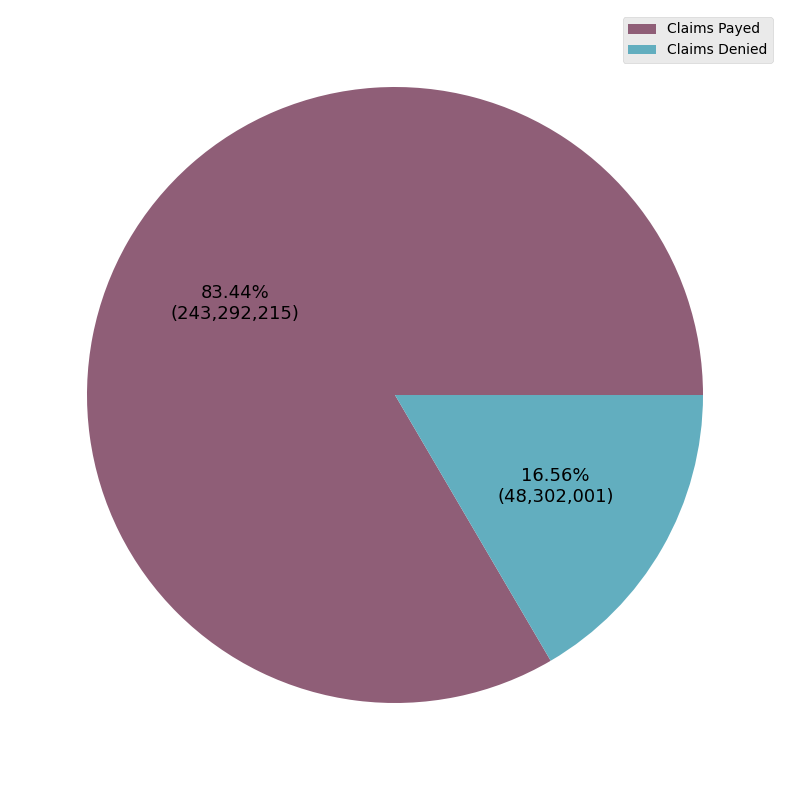
\includegraphics[width=.6\columnwidth]{images/cms_puf/overall_denial_pie.png}
				\caption{Aggregate denial rate across federal marketplace insurers in 2021. Approximately 16\% of all federal marketplace claims were initially denied in 2021, according to CMS TIC PUF data.}
				\label{federal_denial_rate}
			\end{figure}
		\clearpage
	
		\underline{New York Health Care Claims Reports}\\
		
			Among New York insurers, 18\% of all claims submitted in 2022 were initially denied. This data is displayed in Figure \ref{newyorkoveralldenial}.
			
			\begin{figure}[h!]
				\centering
				\textbf{Overall Claims Denial Rate}\\
				\textbf{NY, 2022}\\
				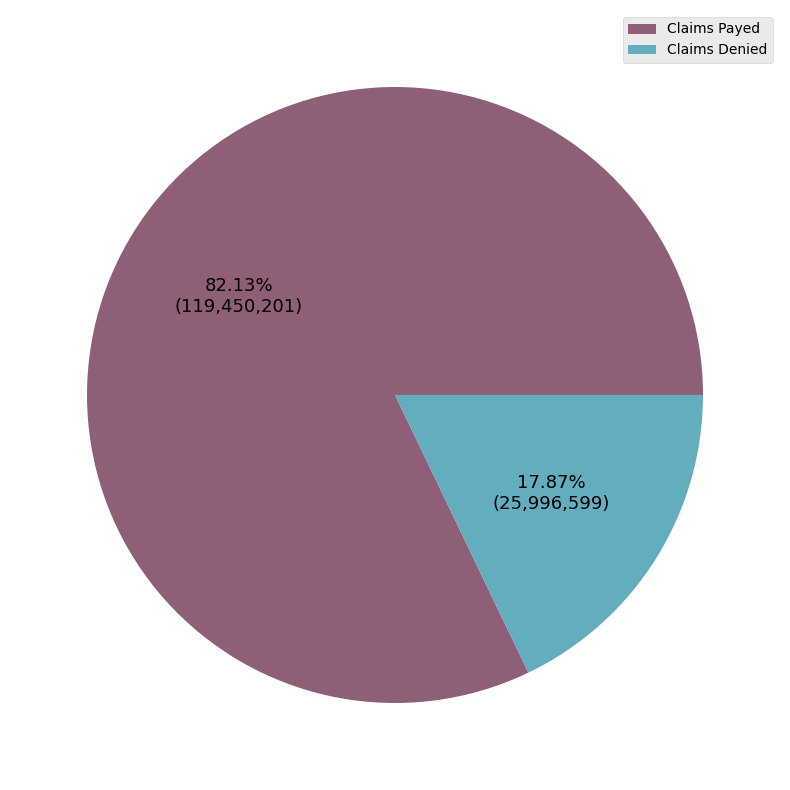
\includegraphics[width=.6\columnwidth]{images/ny_claim_reports/overall_denial_pie.png}
				\caption{Overall denial rate (18\%) among all NY issuers who submitted health care claims reports to the Department of Financial Services in 2022.}
				\label{newyorkoveralldenial}
			\end{figure}
		
		\clearpage
		
		
		\underline{Connecticut Consumer Report Cards}\\
		
		Among Connecticut insurers, 25\% of all claims submitted in 2021 were initially denied. This calculation involved throwing out seemingly spurious data reported for the indemnity plans for one insurer, Connecticare (the report indicates Connecticare had more denials of claims than actual claims received). This data is displayed in Figure \ref{ctoveralldenial}.
		
		\begin{figure}[h!]
			\centering
			\textbf{Overall Claims Denial Rate}\\
			\textbf{CT, 2021}\\
			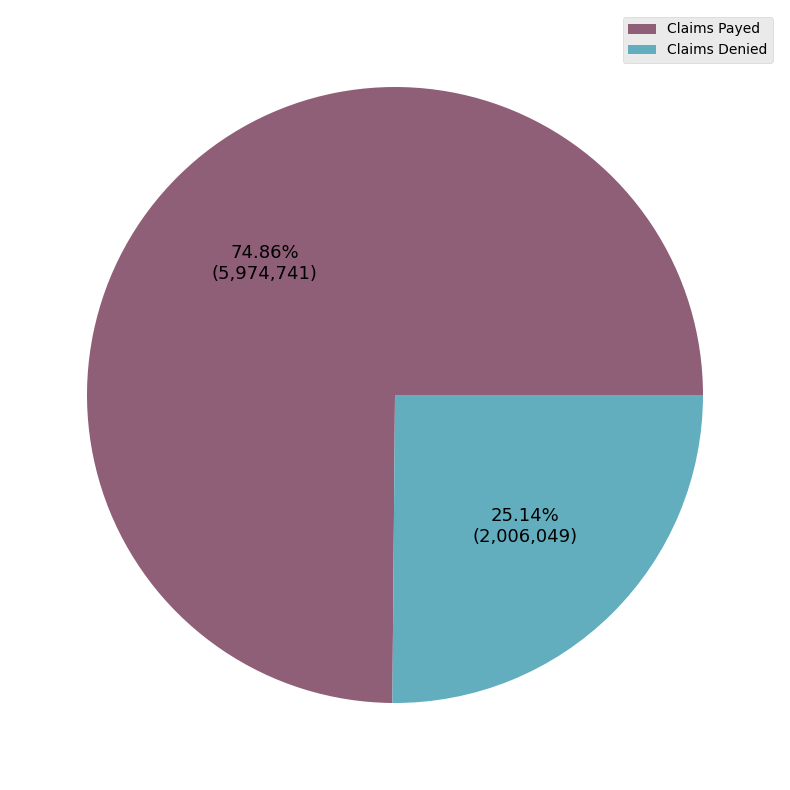
\includegraphics[width=.6\columnwidth]{images/ct_claims/overall_denial_pie.png}
			\caption{Overall claims denial rate in CT consumer report card data.}
			\label{ctoveralldenial}
		\end{figure}
	
	\clearpage
		
		\underline{Pennsylvania Department of Insurance Data}\\
		
		Among Pennsylvania insurers represented in the PA DOI data, approximately 15\% of all claims submitted in 2020 were initially denied, while approximately 13\% of the claims submitted in 2021 were initially denied. This data is displayed in aggregate in Figure \ref{paoveralldenial}.
		
		\begin{figure}[h!]
			\centering
			\textbf{Overall Claims Denial Rate}\\
			\textbf{PA, 2020-2021}\\
			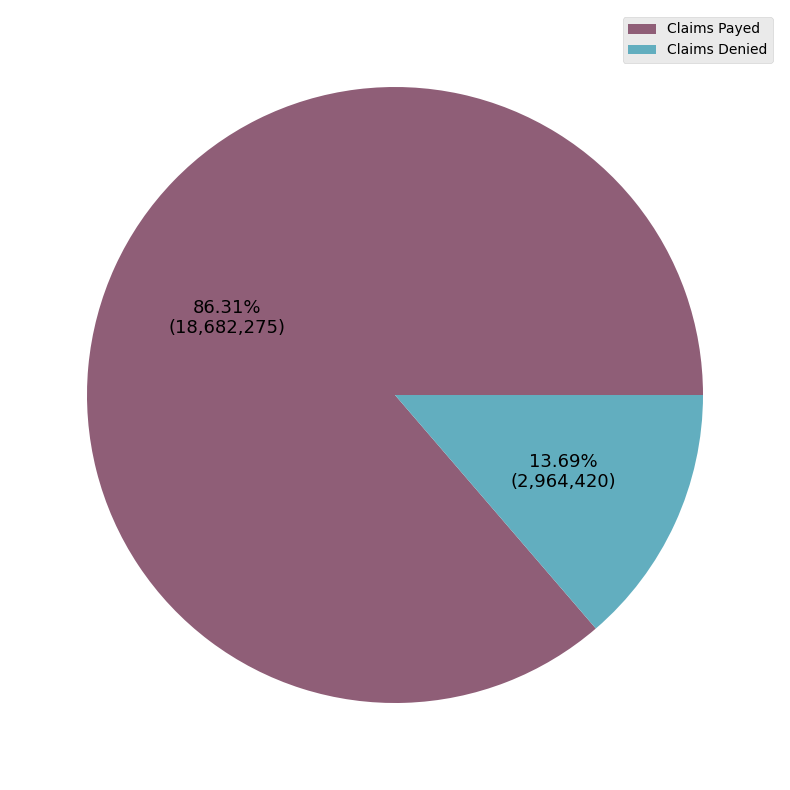
\includegraphics[width=.6\columnwidth]{images/pa_claims/overall_denial_pie.png}
			\caption{Overall claims denial rate in the Pennsylvania Department of Insurance data in 2020 and 2021.}
			\label{paoveralldenial}
		\end{figure}
	\clearpage
		
		
		\subsubsection{Denials By Rationale}
		
		When insurers deny coverage of a claim, they must report their rationale for the denial. The rationales, and the details of how they must be reported to both the insured and regulatory agencies, vary by plan, but typically include a small set of mutually exclusive labels. In each of the datasets that provide denial counts, some metadata regarding the denial rationales is included, though the details vary by dataset.
		
		\underline{CMS Federal Marketplace PUFs}\\
		
		Federal marketplace plans included in the CMS TIC PUF data \emph{sometimes} report rationales for claim denials. Figure \ref{federalrationaledist} shows the categories allowed in the CMS PUF reporting methodology, and their frequency of occurrence in the subset of data which includes rationales.
		
		\begin{figure}[h!]
			\centering
			\textbf{Denials By Rationale}\\
			\textbf{Federal Marketplace, 2021}\\
			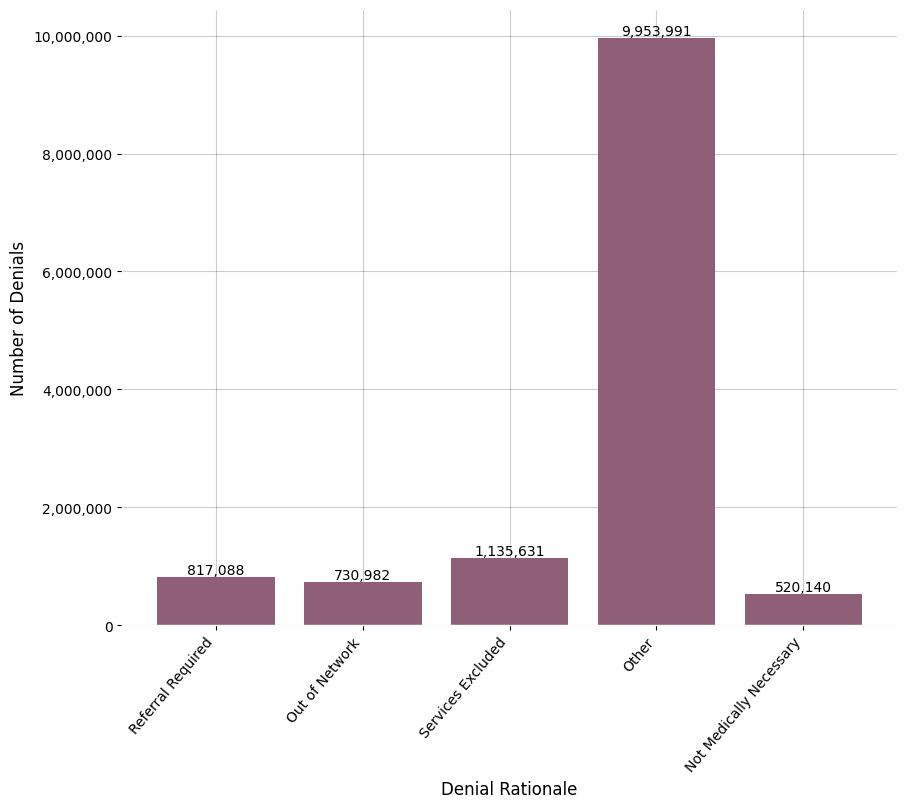
\includegraphics[width=\columnwidth]{images/cms_puf/denials_by_rationale.png}
			\caption{Distribution of claims denial rationales in a subset of the TIC PUF data. }
			\label{federalrationaledist}
		\end{figure}
	
		\clearpage

		Most denials logged in the CMS PUF data are associated with a rationale of ``Other''. This provides little information about the underlying nature of the denials.
		
		Effectively, this reporting scheme allows insurers to withhold reporting the actual reason for a denial to the public if they so choose, since it is not completely clear what is allowed to be reported in the ``Other'' bucket, and there is no strict validation of the reported data. Whether or not insurers actually abuse the system in this way cannot be gleaned from this data alone.
		
		\underline{New York Health Care Claims Reports}\\
		
		The New York Health Care Claims Reports detail the rationales for all of the denials documented in the data, but allow for a different set of available options for denial rationales. These rationales, and their relative frequency of occurrence within the data, are shown in Figure \ref{nyrationaledist}.
		
		\begin{figure}[h!]
			\centering
			\textbf{Denials By Rationale}\\
			\textbf{NY, 2022}\\
			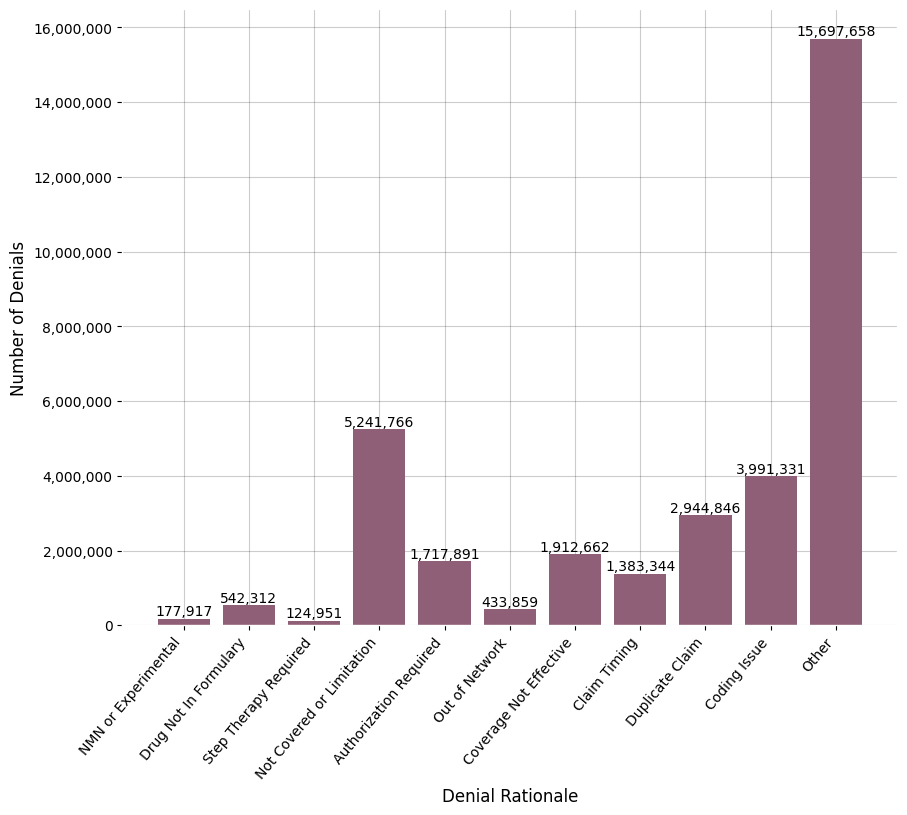
\includegraphics[width=\columnwidth]{images/ny_claim_reports/denial_rationale_dist.png}
			\caption{Distribution of denial rationales for all denials recorded in the health care claims reports submitted to the Department of Financial Services in 2022.}
			\label{nyrationaledist}
		\end{figure}
	
		\clearpage
	
		Again, we see that an ambiguous ``Other'' category is utilized heavily in the reporting. Furthermore, while many of the rationale categories in this dataset are well-defined terms that have consistent, standard meaning across the industry (see e.g. a typical definition of \href{https://en.wikipedia.org/wiki/Step_therapy}{step therapy}), others are ambiguous.
		
		For example, the ``Not Covered or Limitation'' label here is our abbreviation of a label specified in the raw data as ``Not a covered benefit/Exceeds benefit limits (e.g., visit limits)'', which is a broad category that appears to allow for many interpretations, similar to the ``Other'' category. It would be useful to understand more explicitly exactly which subset of denials are being recorded in the ``Not Covered or Limitation'' category, as opposed to the ``Other'' category, or the ``NMN or Experimental'' category, since there is ambiguity and conceptual overlap in each of these concepts. For example, claims deemed to be not medically necessary or experimental are typically a subset of services that are explicitly considered ``not covered'', according to language in insurance contracts.\\
		
		\underline{Connecticut Consumer Report Cards}\\
		
		The Connecticut consumer report cards detail rationales for every denial recorded in the data, but again use a different set of categories, and make liberal use of an ``Other'' category. The data is displayed in Figure \ref{ctrationaledist}.\\
		
		\begin{figure}[h!]
			\centering
			\textbf{Denials By Rationale}\\
			\textbf{CT, 2021}\\
			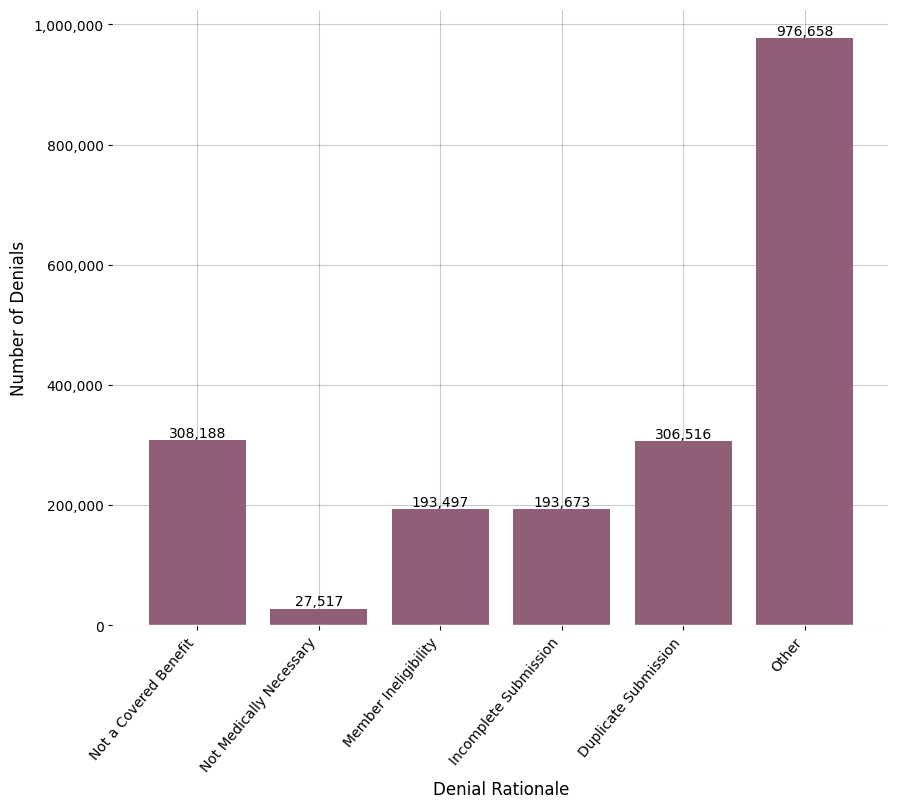
\includegraphics[width=\columnwidth]{images/ct_claims/denials_by_rationale.png}
			\caption{Distribution of denial rationales for all denials in the CT consumer report card data. }
			\label{ctrationaledist}
		\end{figure}
	
		\clearpage
		
		\underline{Pennsylvania Department of Insurance Data}\\
		
		The Pennsylvania Department of Insurance data details rationales only for denials recorded at the plan level in the data (which is the subset corresponding to marketplace claims), but the story remains the same in that the set of permissible rationales in the data is distinct from each other set we've considered. The data is displayed in Figure \ref{parationaledist}.
		
		\begin{figure}[h!]
			\centering
			\textbf{Denials By Rationale}\\
			\textbf{PA, 2020-2021}\\
			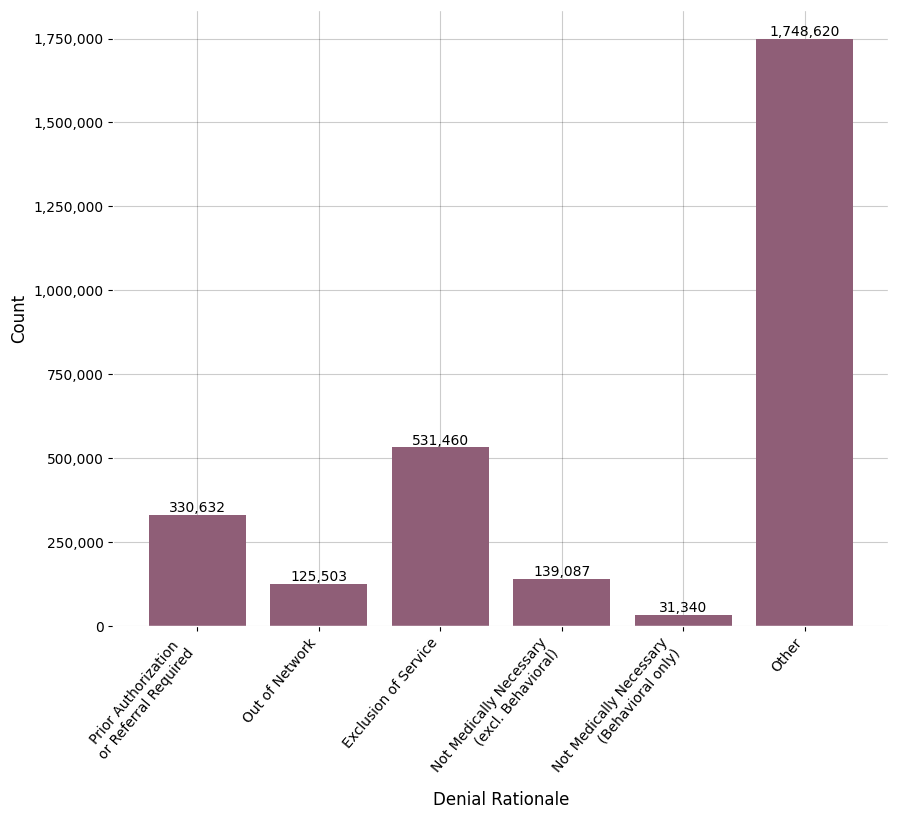
\includegraphics[width=\columnwidth]{images/pa_claims/denial_rationale_dist_2020-2021.png}
			\caption{Distribution of denial rationales for all denials in the PA DOI data.}
			\label{parationaledist}
		\end{figure}
		
		\subsubsection{`Not Medically Necessary' Denial Rates}
		
		Each of the datasets considered provides a category of denial rationale corresponding to purported lack of medical necessity or experimental nature of a service (what we will collectively call \emph{NMN denials}).\\
		
		While NMN denials occur \emph{relatively} infrequently, as Figures 5, 6, 7 and 8 show, they still correspond to a large population of claims in an absolute sense; just for the tiny fraction of all insurance plans covered by the data shown above, for a single plan year, there are more than 700k such claims. Furthermore, they are an important subset of denials in the sense that:\\
		
		\begin{itemize}
			\item Their contractual merit is typically subtle, because it typically involves contractual definitions that themselves reference things like clinical policy bulletins, scientific literature, medical standards, or other external data.
			\item The consequences for such denials can be perilous for patients relying on coverage of treatments for debilitating issues that they would not otherwise be able to afford. This can be true for other rationale categories as well, depending on the categories considered, but is not the case for all categories (e.g. duplicate claims).
		\end{itemize}
	
		For these reasons, we draw attention to aspects of the data pertaining specifically to NMN denials, when possible. Unfortunately, the data is often insufficient to allow much to be ascertained definitively about this subpopulation of denials.\\
		
		One thing we can understand definitively about the subpopulation of NMN denials in these datasets is the rate at which they occur among all claims; these rates can be deduced by reconsidering Figures \ref{federalrationaledist}, \ref{nyrationaledist}, \ref{ctrationaledist}, \ref{parationaledist} but we make the rates explicit in Table  \ref{nmndenialratetable} below.\\
		
		\begin{table}[!ht]
			\centering
			\begin{tabular}{|p{5cm}|p{3cm}|p{4cm}|p{3cm}|}
				\hline
				\textbf{Data Source} & \textbf{NMN Denials} & \textbf{Claims Received \newline With Rationale} & \textbf{NMN Denial \newline Rate}  \\ \hline
				CMS TIC PUF (2021) & 520,140 & 13,157,832 & .0395 \\ \hline
				NY Health Care Claims Reports (2022) & 177,881 & 34,168,504 & 	.0052 \\ \hline
				Connecticut Consumer Report Card (2021) & 27,517 & 2,006,049 &  .0137 \\ \hline
				Pennsylvania DOI Data (2020) & 104,396 & 10,451,280 &  .0099 \\ \hline
				Pennsylvania DOI Data (2021) & 66,031 & 	9,494,221 &  	.0069 \\ \hline
			\end{tabular}
			\caption{NMN Denial Rates}
			\label{nmndenialratetable}
		\end{table}
		
		
		Unsurprisingly we see that NMN denial rates are orders of magnitude smaller than overall denial rates; however, it is interesting to note that there is significant variation in the overall NMN denial rate across these datasets. One contributing factor is surely the lack of standardization in reporting methodologies, such as the variation in the set of denial rationales permissible in the reported data. It is unclear to what extent the actual denial rates relating to medical necessity would vary across these datasets if one were to correct for reporting inconsistencies. \\
		
		
		\subsubsection{Denials By Insurer}
		
		Each of the datasets reporting denials includes breakdowns of the claims received and claims denied by insurer. It is informative to understand how the aggregate denial rates and NMN denial rates vary by insurer within each dataset.
		
		We note at the outset that while it is informative to understand how various distributions vary by insurer, there are many subtleties lurking behind such breakdowns, just as there were for denial rationales. For example, different insurers may have different distributions of plan network types (e.g. relative fraction of consumers on HMO, EPO, PPO, and POS plans), and as a result insurer denial differences might partially be a reflection of the differences in those plan type distributions. Or, alternatively, two insurers might have identical plan type distributions and administration practices, but have a different list of drugs for which they require prior-authorization, with one list containing some much more commonly utilized drugs. Given such subtleties which the data does not allow us to address, it is difficult to definitively understand the cause of the phenomenology we observe in differences across insurers.
		
		In the same vein, the distribution across insurers of denials whose rationale specifically involves the experimental nature of a treatment, rather than another medical necessity rationale, could be influenced by many things, in addition to the raw counts of claims. In particular, one would expect that wealthy and renowned hospital systems conducting cutting edge research would be more likely than others to attempt truly experimental or novel services for their patients in need, and that such properties of a hospital are correlated with other properties, such as proximity to a major city and research center. As a result, health insurance companies with networks that overlap certain geographic areas, or that include certain hospitals, might receive a distribution of claims with a relatively high share that could be interpreted as involving experimental treatments, when compared to distributions received by other insurance companies. In such a context, it would be inappropriate to make an inference about how experimental claims denial processes vary by insurer from experimental claims denial rates alone.
		
		As with all of the data we examine in this article, there are many subtleties that make it difficult to draw conclusions without more information. We make suggestions to address this troubling predicament in the concluding \hyperref[recommendations]{recommendations} section.

		
		\underline{CMS Federal Marketplace PUFs}\\
		
		Figures \ref{fedinsurerclaims}, \ref{fedinsurerdenialrates}, and \ref{fedinsurernmndenialrates} show the overall claims counts, denial rates, and NMN denial rates for the 10 issuers in the CMS TIC PUF Federal Marketplace data with the highest claims volume.
		
		
		\begin{figure}[h!]
			\centering
			\textbf{Claims Count By Insurer}\\
			\textbf{Federal Marketplace, 2021}\\
			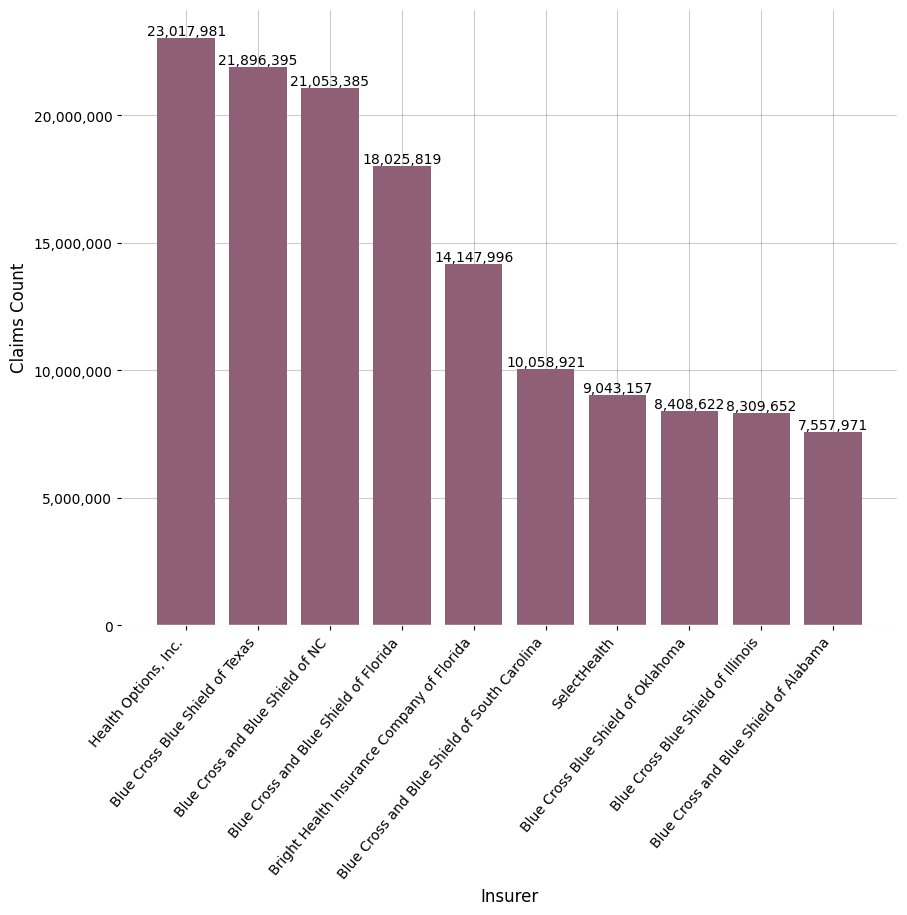
\includegraphics[width=\columnwidth]{images/cms_puf/claims_by_insurer.png}
			\caption{Claims received for the 10 issuers with the largest number of claims adjudicated in the 2021 CMS TIC PUF data.}
			\label{fedinsurerclaims}
		\end{figure}
	
		\clearpage
	
	
		\begin{figure}[h!]
			\centering
			\textbf{Denial Rate By Insurer}\\
			\textbf{Federal Marketplace, 2021}\\
			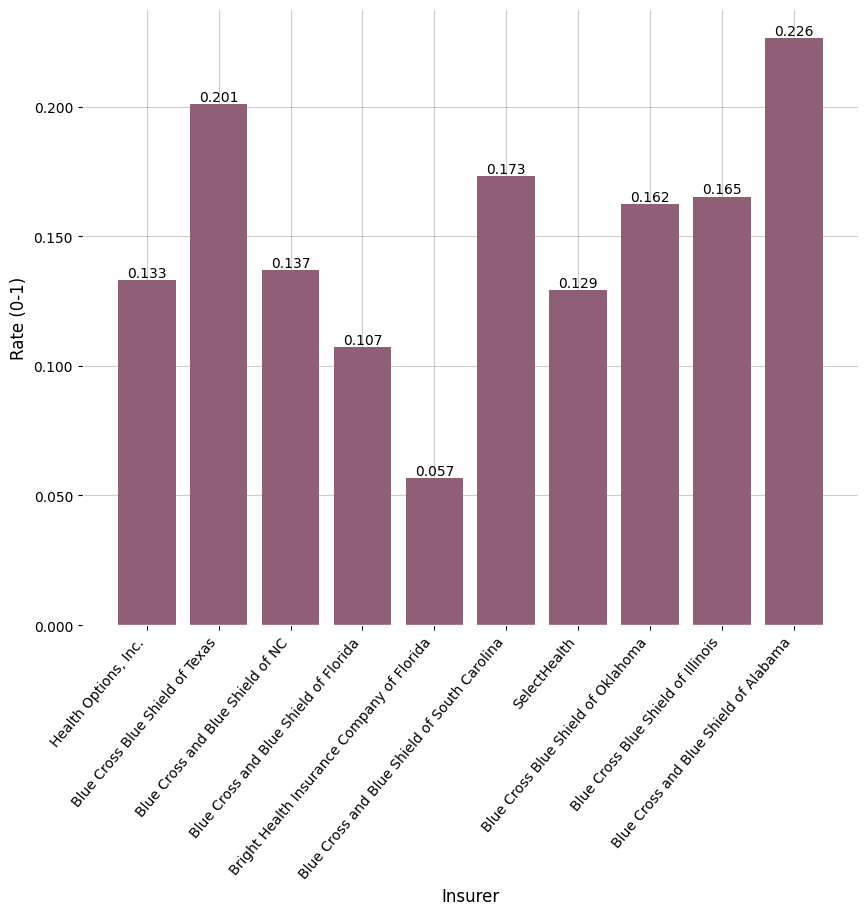
\includegraphics[width=\columnwidth]{images/cms_puf/denial_rate_by_insurer.png}
			\caption{Overall claims denial rates for the 10 issuers with the largest number of claims adjudicated in the 2021 CMS TIC PUF data.}
			\label{fedinsurerdenialrates}
		\end{figure}
	
		\clearpage
		
		\begin{figure}[h!]
			\centering
			\textbf{NMN Denial Rate By Insurer}\\
			\textbf{Federal Marketplace, 2021}\\
			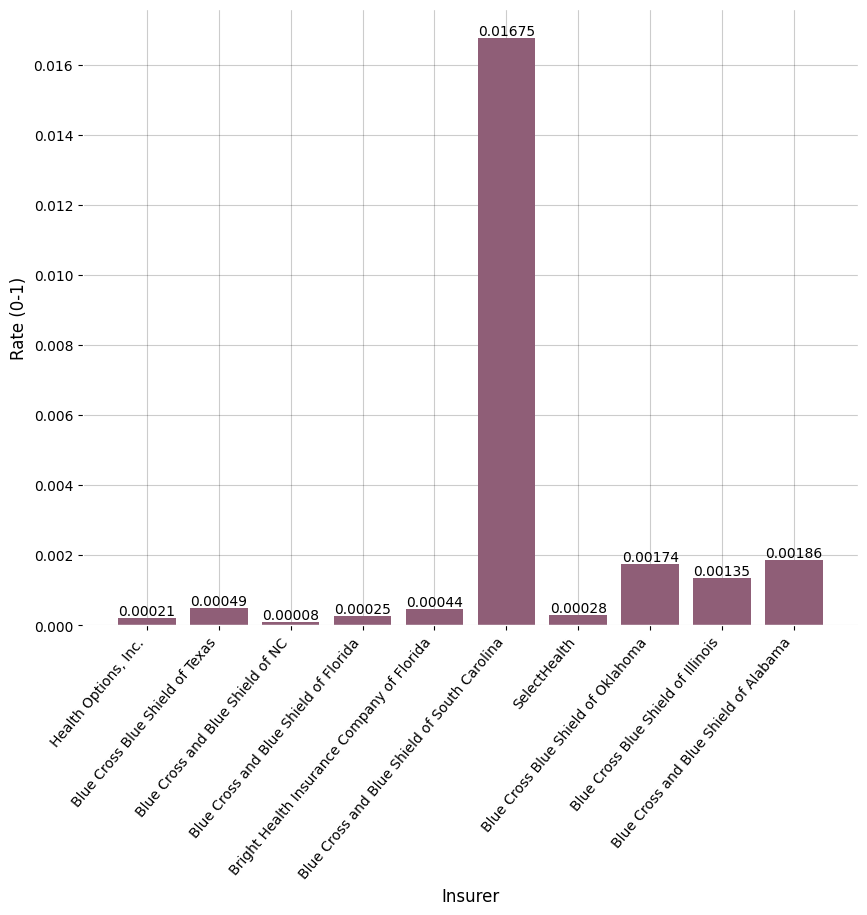
\includegraphics[width=\columnwidth]{images/cms_puf/nmn_denial_rate_by_insurer.png}
			\caption{NMN (including experimental) denial rates for the 10 issuers with the largest number of claims adjudicated in the 2021 CMS TIC PUF data.}
			\label{fedinsurernmndenialrates}
		\end{figure}
	
		Among the largest federal marketplace issuers of 2021, as measured by claims received, Blue Cross Blue Shield of South Carolina has an NMN denial rate roughly two to three orders of magnitude larger than the others. It is unclear what drives this phenomenon.
		
		Figure \ref{feddenialrationalesbyinsurer} shows a heatmap displaying the distribution of denial rationales among these same highest volume insurers.
		
		\begin{figure}[h!]
			\centering
			\textbf{Denial Rationales By Insurer}\\
			\textbf{Federal Marketplace, 2021}\\
			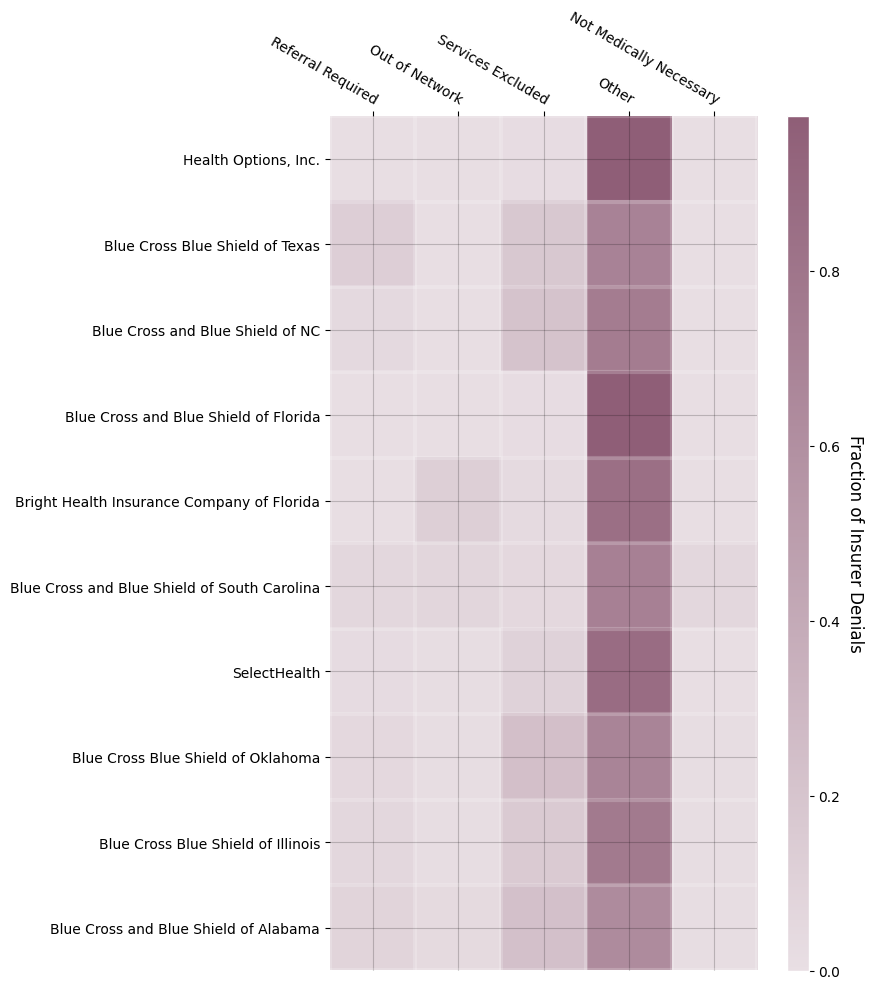
\includegraphics[width=\columnwidth]{images/cms_puf/insurer_vs_denial_cat.png}
			\caption{Distribution of denial rationales for the 10 issuers with the largest number of claims adjudicated in the 2021 CMS TIC PUF data. The color indicates the fraction of all denials for a given insurer that were coded with a particular rationale (i.e. rows sum to 1). }
			\label{feddenialrationalesbyinsurer}
		\end{figure}
	
		\clearpage
		
		
		
		\underline{New York Health Care Claims Reports}\\
		
				Figures \ref{nyinsurerclaims}, \ref{nyinsurerdenialrates}, and \ref{nyinsurernmndenialrates} show the overall claims counts, denial rates, and NMN denial rates for the 10 issuers in the New York Health Care Claims Reports data with the highest claims volume.
		
		\begin{figure}[h!]
			\centering
			\textbf{Claims Count By Insurer}\\
			\textbf{NY, 2022}\\
			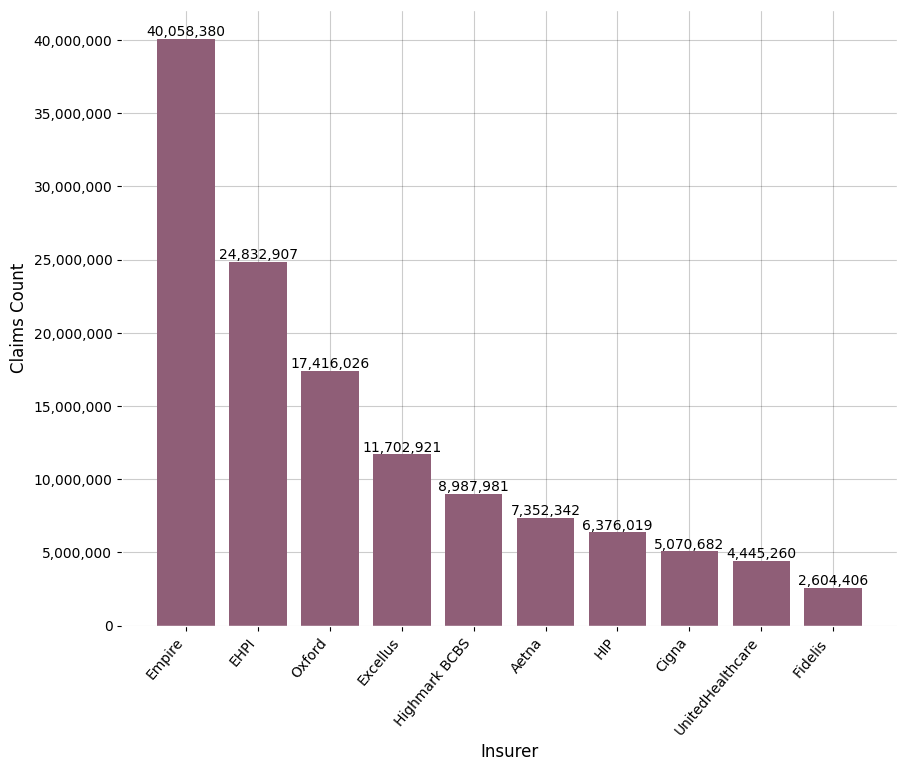
\includegraphics[width=\columnwidth]{images/ny_claim_reports/claims_by_insurer.png}
			\caption{Claims received for the 10 issuers with the largest number of claims adjudicated in the 2022 Department of Financial Services claims report data.}
			\label{nyinsurerclaims}
		\end{figure}
		
		\clearpage
		
		
		\begin{figure}[h!]
			\centering
			\textbf{Denial Rate By Insurer}\\
			\textbf{NY, 2022}\\
			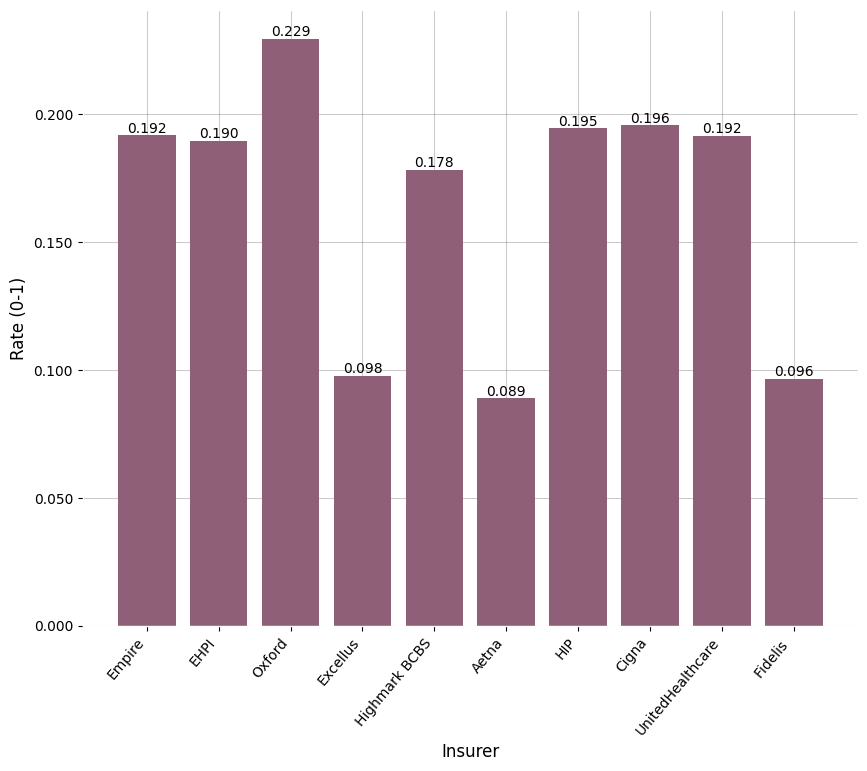
\includegraphics[width=\columnwidth]{images/ny_claim_reports/denial_rate_by_insurer.png}
			\caption{Overall claims denial rates for the 10 issuers with the largest number of claims adjudicated in the 2022 Department of Financial Services claims report data.}
			\label{nyinsurerdenialrates}
		\end{figure}
		
		\clearpage
		
		\begin{figure}[h!]
			\centering
			\textbf{NMN Denial Rate By Insurer}\\
			\textbf{NY, 2022}\\
			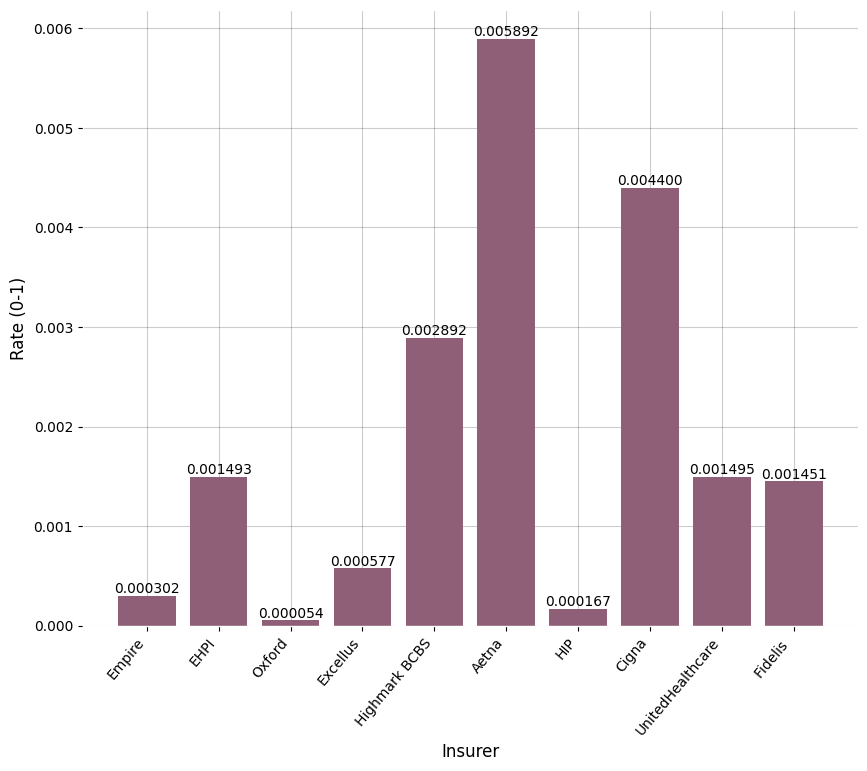
\includegraphics[width=\columnwidth]{images/ny_claim_reports/nmn_denial_rate_by_insurer.png}
			\caption{NMN (including experimental) denial rates for the 10 issuers with the largest number of claims adjudicated in the 2022 Department of Financial Services claims report data.}
			\label{nyinsurernmndenialrates}
		\end{figure}
	
		
		Figure \ref{nydenialrationalesbyinsurer} shows a heatmap displaying the distribution of denial rationales among these same highest volume insurers.
		
		\begin{figure}[h!]
			\centering
			\textbf{Denial Rationales By Insurer}\\
			\textbf{NY, 2022}\\
			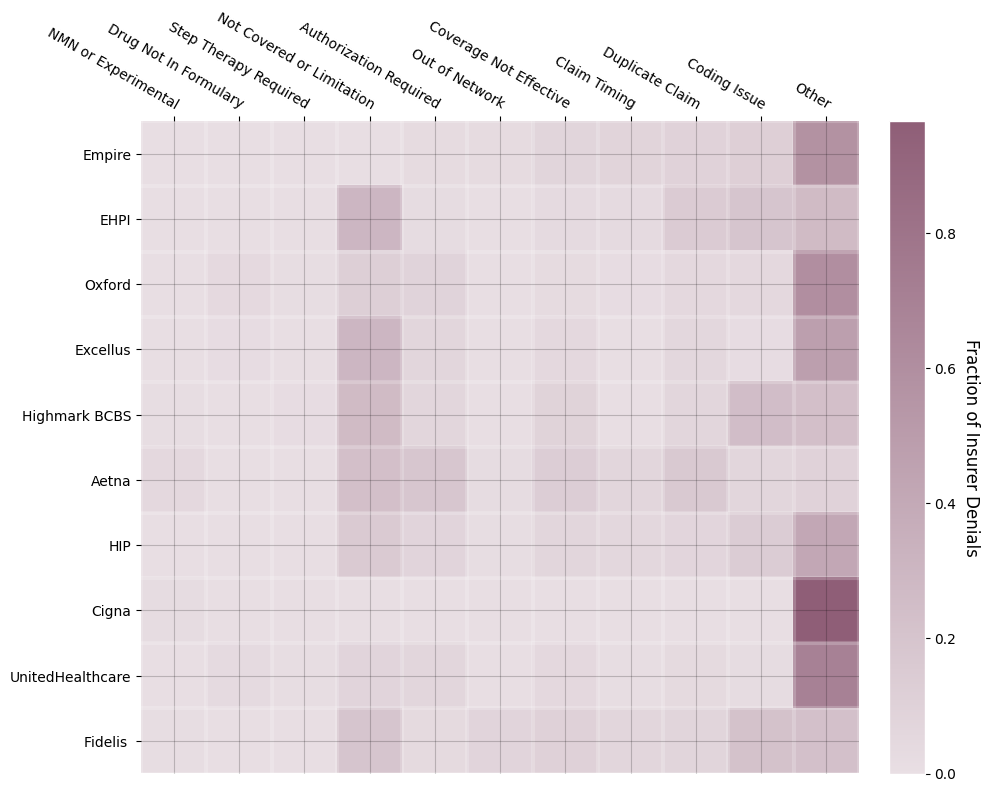
\includegraphics[width=\columnwidth]{images/ny_claim_reports/insurer_vs_denial_cat.png}
			\caption{Distribution of denial rationales for the 10 issuers with the largest number of claims adjudicated in the 2022 Department of Financial Services claims report data. The color indicates the fraction of all denials for a given insurer that were coded with a particular rationale (i.e. rows sum to 1).}
			\label{nydenialrationalesbyinsurer}
		\end{figure}
		
		\clearpage
		


		
		\underline{Connecticut Consumer Report Cards}\\
		
		
		Figures \ref{ctinsurerclaims}, \ref{ctinsurerdenialrates}, and \ref{ctinsurernmndenialrates} show the overall claims counts, denial rates, and NMN denial rates for the 10 issuers in the Connecticut Consumer Report Card data with the highest claims volume.

		\begin{figure}[h!]
			\centering
			\textbf{Claims Count By Insurer}\\
			\textbf{CT, 2021}\\
			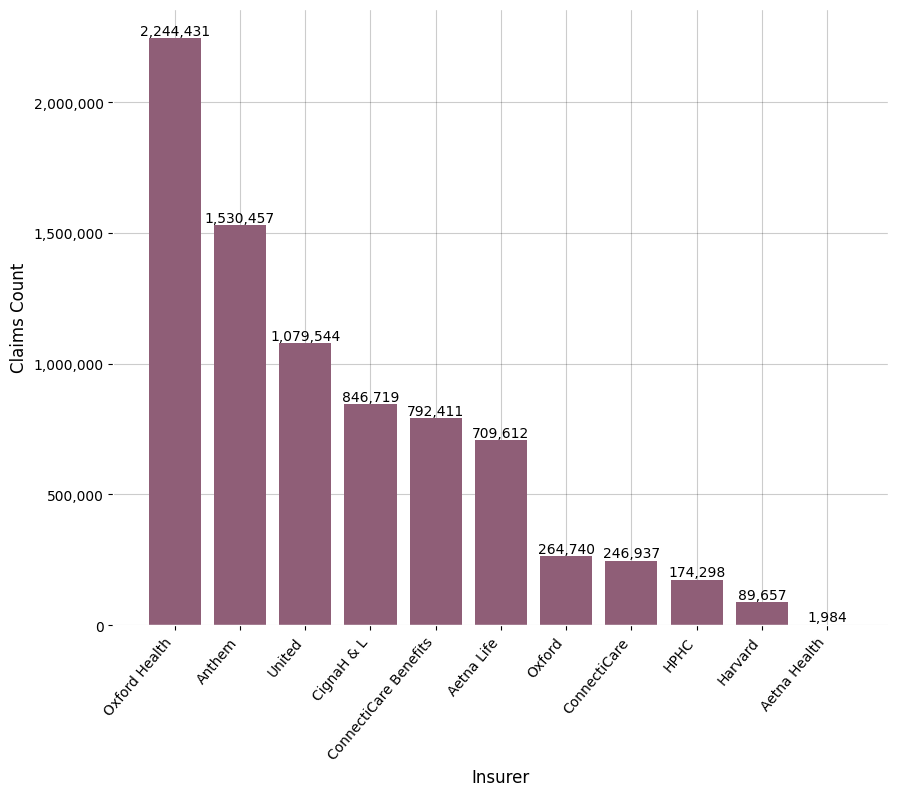
\includegraphics[width=\columnwidth]{images/ct_claims/claims_by_insurer.png}
			\caption{Claims received for all issuers in the CT consumer report card data.}
			\label{ctinsurerclaims}
		\end{figure}
		
		\clearpage
		
		
		\begin{figure}[h!]
			\centering
			\textbf{Denial Rate By Insurer}\\
			\textbf{CT, 2021}\\
			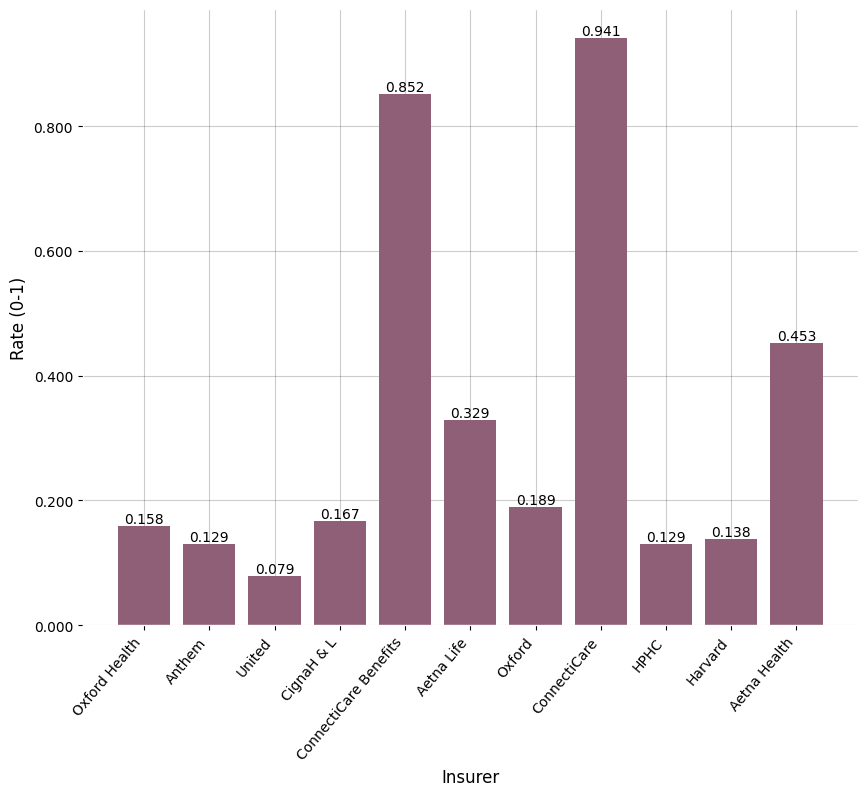
\includegraphics[width=\columnwidth]{images/ct_claims/denial_rate_by_insurer.png}
			\caption{Overall claims denial rates for all issuers in the CT consumer report card data.}
			\label{ctinsurerdenialrates}
		\end{figure}
		
		\clearpage
		
		\begin{figure}[h!]
			\centering
			\textbf{NMN Denial Rate By Insurer}\\
			\textbf{CT, 2021}\\
			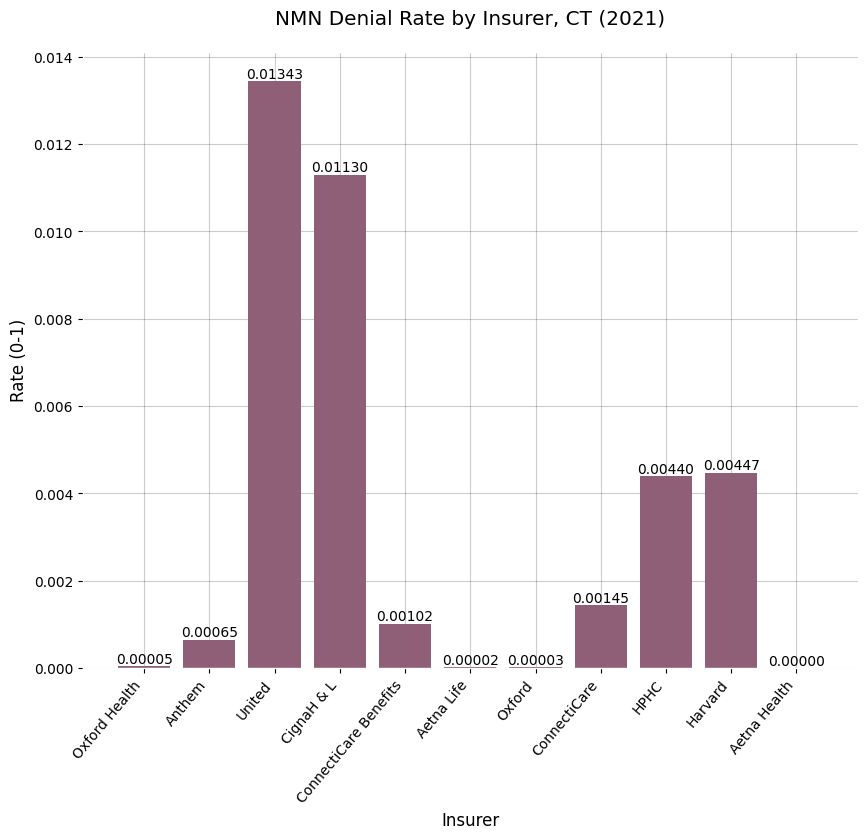
\includegraphics[width=\columnwidth]{images/ct_claims/nmn_denial_rate_by_insurer.png}
			\caption{NMN (including experimental) denial rates for all issuers in the CT consumer report card data.}
			\label{ctinsurernmndenialrates}
		\end{figure}
	
		Figure \ref{ctinsurerdenialrates} shows odd and potentially spurious data that indicates one set of issuers, 'ConnectiCare Benefits' and 'ConnectiCare', have extremely high claims denial rates above 85\%. We suspect this is a reporting error in the raw data, but we show it here because we cannot be sure of that fact. We were unable to find further information about this anomaly.
		
		Figure \ref{ctdenialrationalesbyinsurer} shows a heatmap displaying the distribution of denial rationales among these same highest volume insurers.

		
		\begin{figure}[h!]
			\centering
			\textbf{Denial Rationales By Insurer}\\
			\textbf{CT, 2021}\\
			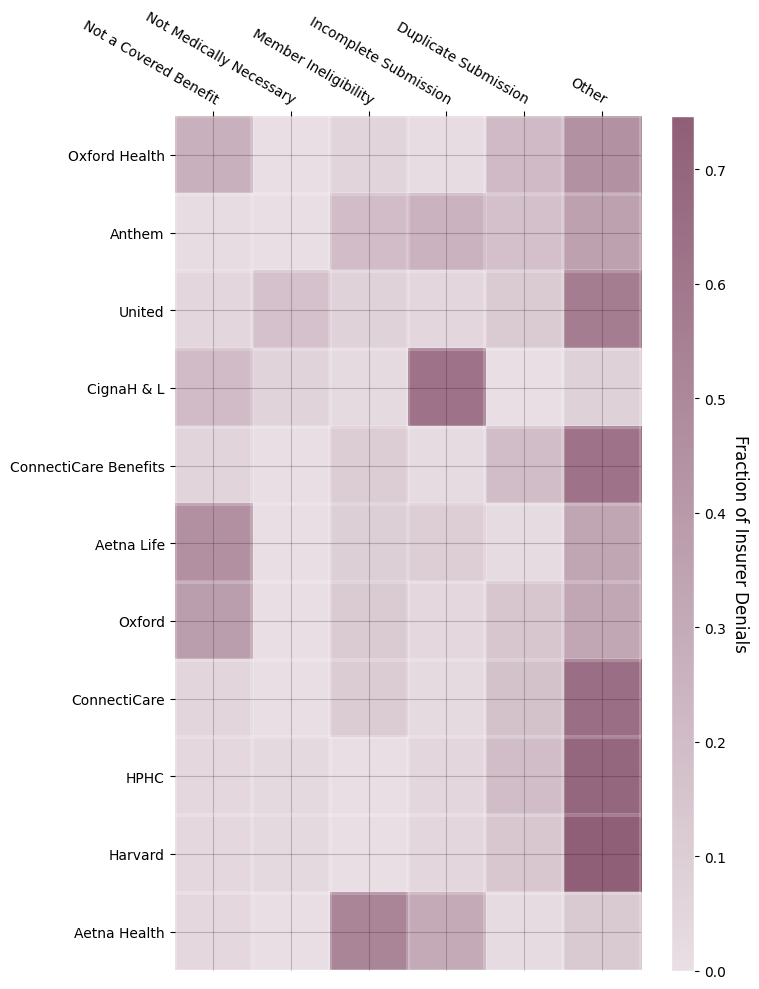
\includegraphics[width=\columnwidth]{images/ct_claims/insurer_vs_denial_cat.png}
			\caption{Distribution of denial rationales for all issuers in the CT consumer report card data. The color indicates the fraction of all denials for a given insurer that were coded with a particular rationale (i.e. rows sum to 1).}
			\label{ctdenialrationalesbyinsurer}
		\end{figure}
		
		\clearpage
		
		
		\underline{Pennsylvania Department of Insurance Data} \\
		
		
		Figures \ref{painsurerclaims}, \ref{painsurerdenialrates}, and \ref{painsurernmndenialrates} show the overall claims counts, denial rates, and NMN denial rates for the 10 issuers in the Pennsylvania Department of Insurance Data data with the highest claims volume.
	

		\begin{figure}[h!]
			\centering
			\textbf{Claims Count By Insurer}\\
			\textbf{PA, 2020-2021}\\
			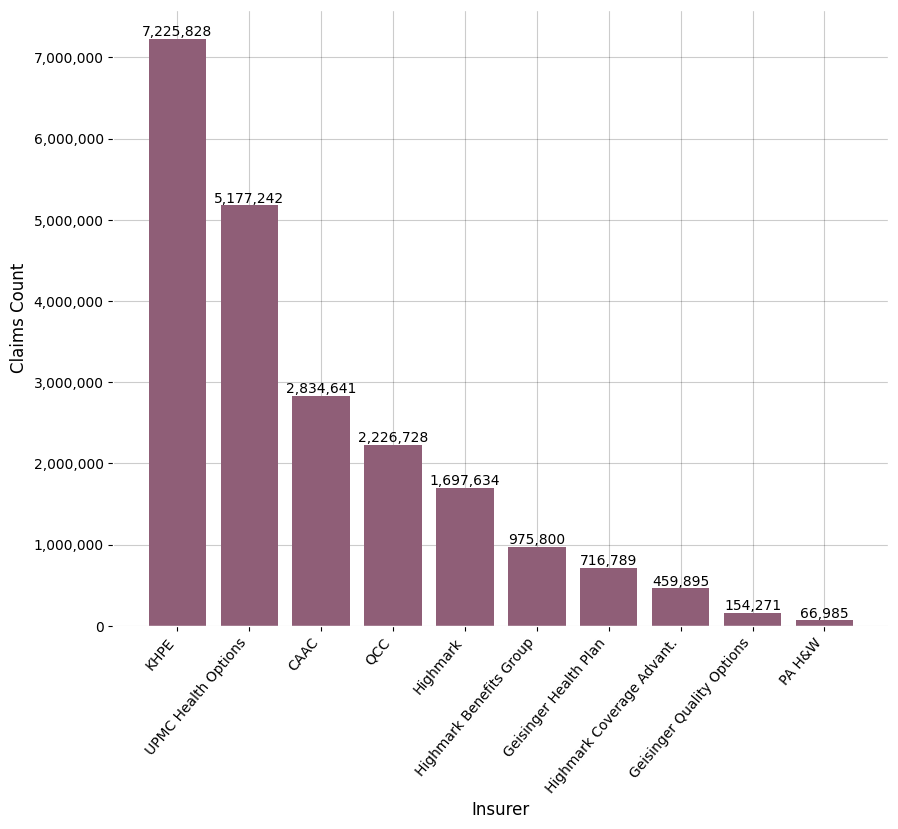
\includegraphics[width=\columnwidth]{images/pa_claims/claims_by_insurer.png}
			\caption{Claims received for all issuers in the PA DOI data.}
			\label{painsurerclaims}
		\end{figure}
		
		\clearpage
		
		
		\begin{figure}[h!]
			\centering
			\textbf{Denial Rate By Insurer}\\
			\textbf{PA, 2020-2021}\\
			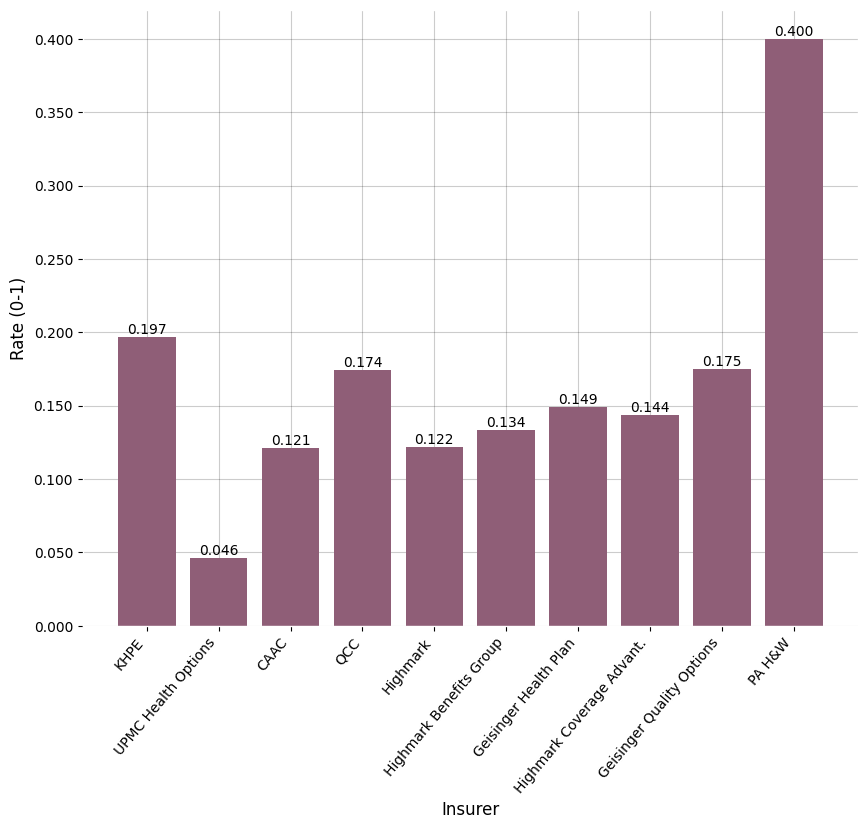
\includegraphics[width=\columnwidth]{images/pa_claims/denial_rate_by_insurer.png}
			\caption{Overall claims denial rates for all issuers in the PA DOI data.}
			\label{painsurerdenialrates}
		\end{figure}
		
		\clearpage
		
		\begin{figure}[h!]
			\centering
			\textbf{NMN Denial Rate By Insurer}\\
			\textbf{PA, 2020-2021}\\
			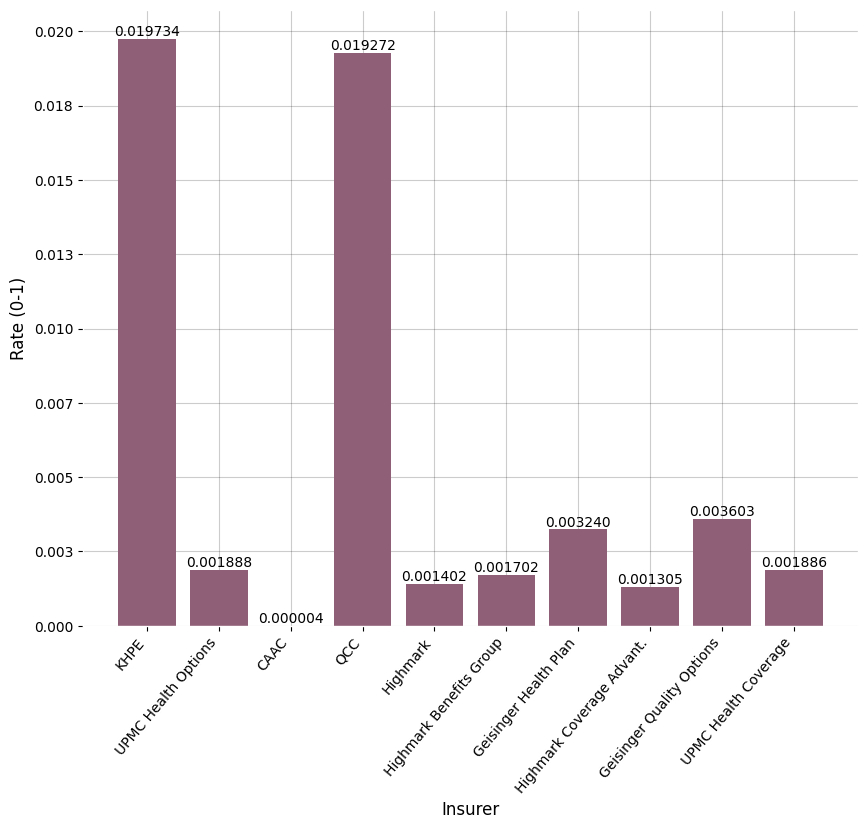
\includegraphics[width=\columnwidth]{images/pa_claims/nmn_denial_rate_by_insurer.png}
			\caption{NMN (including experimental) denial rates for all issuers in the PA DOI data.}
			\label{painsurernmndenialrates}
		\end{figure}
		
		
		Figure \ref{padenialrationalesbyinsurer} shows a heatmap displaying the distribution of denial rationales among these same highest volume insurers.
		
		
		\begin{figure}[h!]
			\centering
			\textbf{Denial Rationales By Insurer}\\
			\textbf{PA, 2020-2021}\\
			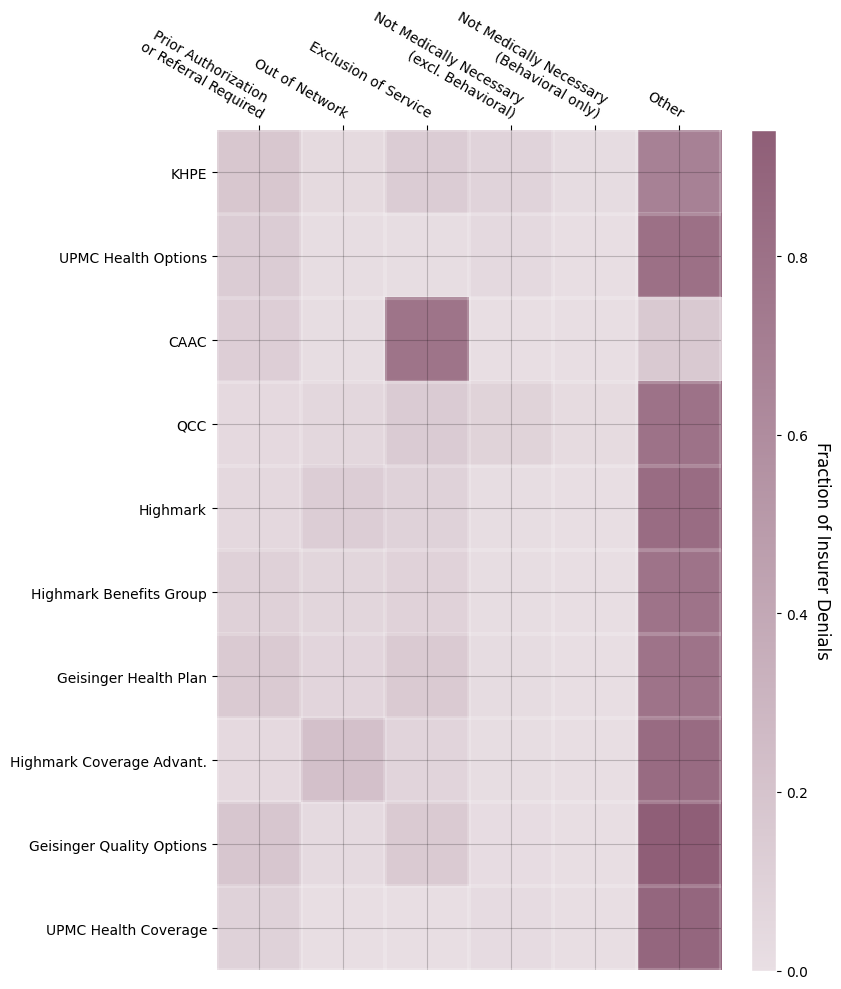
\includegraphics[width=\columnwidth]{images/pa_claims/insurer_vs_denial_cat.png}
			\caption{Distribution of denial rationales for all issuers in the PA DOI data who report denial rationales. The color indicates the fraction of all denials for a given insurer that were coded with a particular rationale (i.e. rows sum to 1).}
			\label{padenialrationalesbyinsurer}
		\end{figure}
		
		\clearpage
		
		
		
		\subsubsection{Dataset Specific Considerations}
		
		Since the datasets do not report claims and denial information in a standard or consistent way, there are many interesting considerations that can be made for only some of the datasets. Here we present dataset specific considerations relating to claims and denial distributions.
		
		
		
		\underline{CMS Federal Marketplace PUFs}\\
		
		The CMS TIC PUFs provide many pieces of metadata associated with individual plans, and their corresponding aggregate claims data, that allow denials to be broken down across additional categories.
		
		At a high level, we can calculate the overall denial rate for each \emph{issuer} (an insurer's \href{https://www.law.cornell.edu/definitions/uscode.php?width=840&height=800&iframe=true&def_id=26-USC-392827901-289353966&term_occur=1&term_src=}{state specific entity}), by calculating the ratio of all claims denied by that issuer, to the claims received by that issuer (across all their plans).
		
		Figure \ref{federalissuerdenialdist} shows the distribution of such issuer denial rates across issuers represented in the 2021 CMS TIC PUF data. The distribution is bimodal, with a large majority of issuers comprising a contingency with aggregate denial rates between 0\% to 30\%, and a small contingency of issuers maintaining aggregate denial rates between 35\% to 50\%. While we could compute such a distribution for the other datasets as well, the number of issuers involved is too small to infer much from the resulting distribution. Here, however, the distribution sheds some light on how denial rates vary by issuer.
		
		
		\begin{figure}[h!]
			\centering
			\textbf{Denial Rates}\\
			\textbf{Federal Marketplace Issuers, 2021}\\
			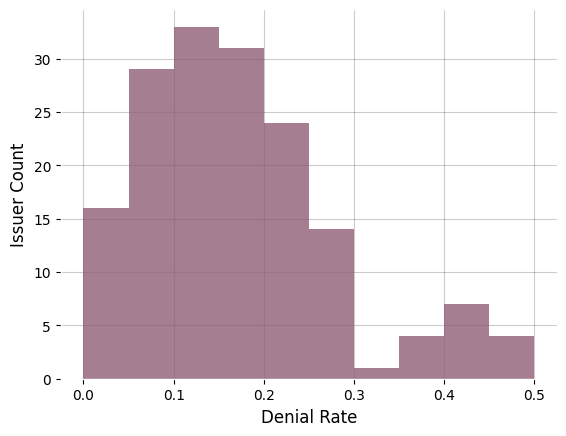
\includegraphics[width=\columnwidth]{images/cms_puf/denial_rates_all_insurers.png}
			\caption{Distribution of claims denial rates across federal marketplace issuers in 2021. Across issuers, denial rates vary from approximately 0\% to 50\%.}
			\label{federalissuerdenialdist}
		\end{figure}
	
		\clearpage
	
	
		Each plan reported in the data also has metadata associated with it. Figures \ref{federaldenialratesbyplantype} and \ref{federaldenialratesbymetallevel} contain plots that show the distribution of individual plan denial rates, as a function of two properties of plans:
		
		\begin{itemize}
			\item \emph{Plan administration and network type}
			
				Health insurance plans utilize different \href{https://www.healthcare.gov/choose-a-plan/plan-types/}{network and administration policy types}, which dictate things like which providers are considered part of your plans preferred network, and how you must seek certain types of care and services (e.g. by obtaining referrals for specialist visits). Some common policy types include Exclusive Provider Organizations (EPOs), Health Maintenance Organizations (HMOs), Point of Service (POS), and Preferred Provider Organizations (PPOs).
			
			\item \emph{Metal level}
			
			
				Federal marketplace plans are partitioned according to so-called \href{https://www.healthcare.gov/choose-a-plan/plans-categories/}{plan categories}, which are mostly named by metals. The categories are Catastrophic, Bronze, Bronze Expanded, Silver, Gold and Platinum. Generally, plans that fall into a more precious metal category have higher premiums, but cover a larger fraction of the cost of care when coverage kicks in. Catastrophic plans, as the name suggests, typically only provide coverage for catastrophic situations.
		\end{itemize}
	
		The data show that:
		
		\begin{itemize}
			\item A larger fraction of EMO and HMO plans have denial rates between 30\% to 50\% than do PPO and POS plans.
			\item Only platinum level plans completely lack a contingent of 30\% to 50\% denial rate constituents.
		\end{itemize}
	
		
				\begin{figure}
					\centering
					\textbf{Denial Rates By Plan Type}\\
					\textbf{Federal Marketplace, 2021}\\
					\vspace{3em}
					\centering
					\begin{subfigure}[t]{0.49\textwidth}
						\centering
						\textbf{PPO}
						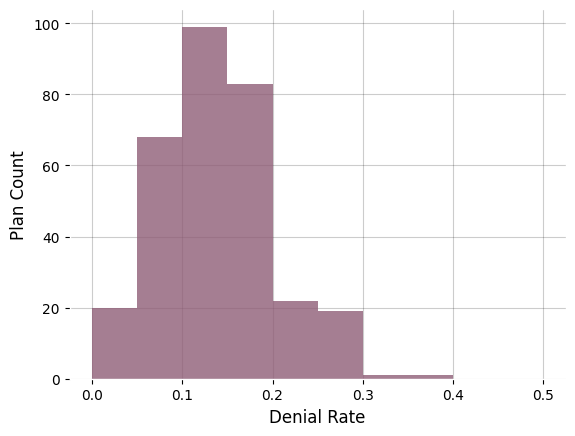
\includegraphics[width=\textwidth]{images/cms_puf/PPO_dist.png}
					\end{subfigure}
					\hfill
					\begin{subfigure}[t]{0.49\textwidth}
						\centering
						\textbf{EPO}
						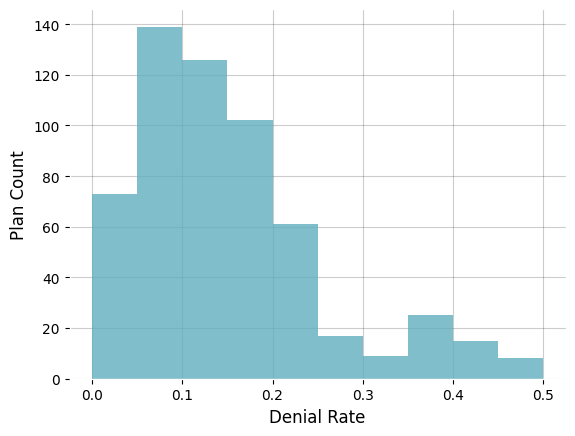
\includegraphics[width=\textwidth]{images/cms_puf/EPO_dist.png}
					\end{subfigure}
					\hfill
					\vspace{1em}
					\begin{subfigure}[t]{0.49\textwidth}
						\centering
						\textbf{POS}
						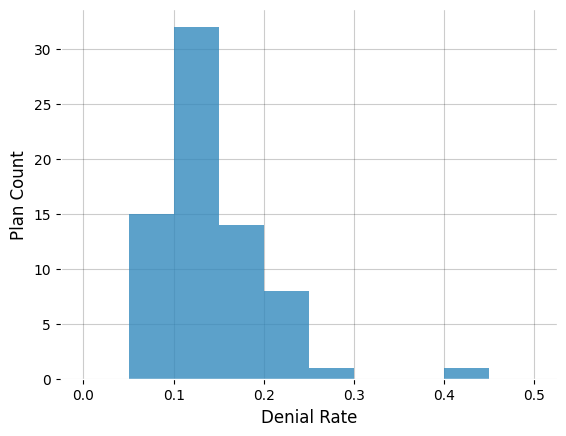
\includegraphics[width=\textwidth]{images/cms_puf/POS_dist.png}
					\end{subfigure}
					\hfill
					\begin{subfigure}[t]{0.49\textwidth}
						\centering
						\textbf{HMO}
						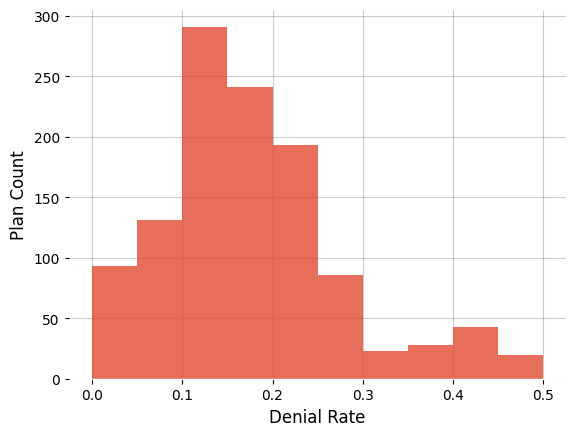
\includegraphics[width=\textwidth]{images/cms_puf/HMO_dist.png}
					\end{subfigure}
				
					\caption{Distribution of claims denial rates broken down by plan types.}
					\label{federaldenialratesbyplantype}
			\end{figure}
		
			\clearpage
			
			
			\begin{figure}
				\centering
				\textbf{Denial Rates By Metal Level}\\ 
				\textbf{Federal Marketplace, 2021}\\
				\vspace{3em}
				\centering
				\begin{subfigure}[t]{0.49\textwidth}
					\centering
					\textbf{Catastrophic}
					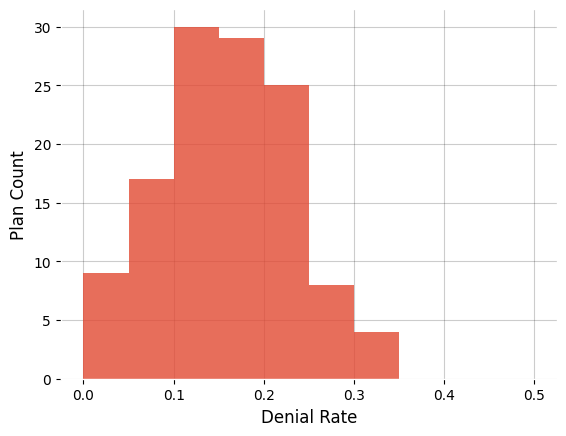
\includegraphics[width=\textwidth]{images/cms_puf/Catastrophic_dist.png}
				\end{subfigure}
				\hfill
				\begin{subfigure}[t]{0.49\textwidth}
					\centering
					\textbf{Bronze}
					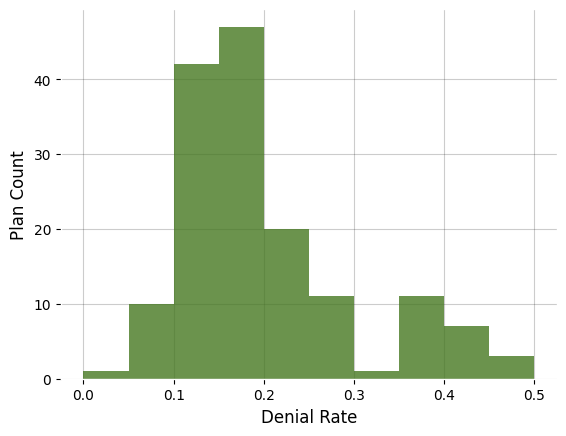
\includegraphics[width=\textwidth]{images/cms_puf/Bronze_dist.png}
				\end{subfigure}
				\hfill
				\vspace{1em}
				\begin{subfigure}[t]{0.49\textwidth}
					\centering
					\textbf{Bronze Expanded}
					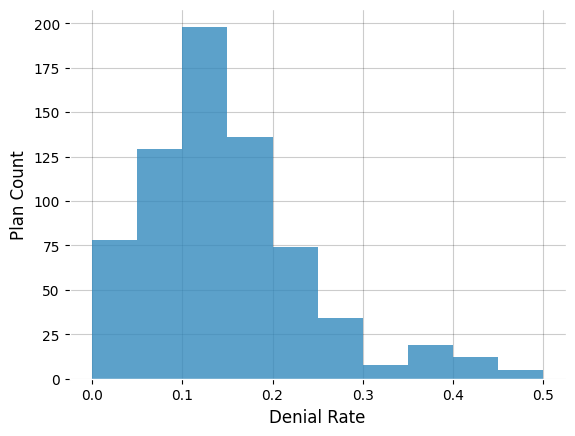
\includegraphics[width=\textwidth]{images/cms_puf/Bronze Expanded_dist.png}
				\end{subfigure}
				\hfill
				\begin{subfigure}[t]{0.49\textwidth}
					\centering
					\textbf{Silver}
					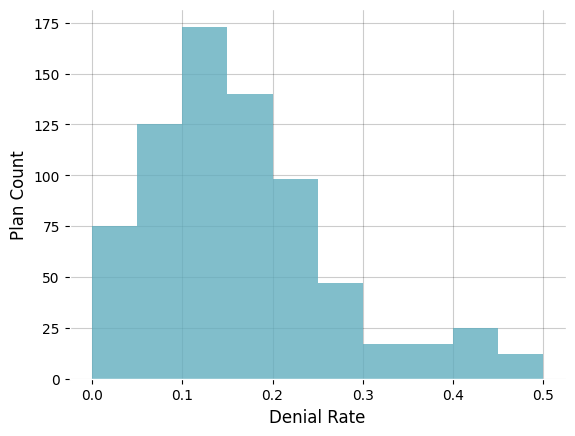
\includegraphics[width=\textwidth]{images/cms_puf/Silver_dist.png}
				\end{subfigure}
				\hfill
				\vspace{1em}
				\begin{subfigure}[t]{0.49\textwidth}
					\centering
					\textbf{Gold}
					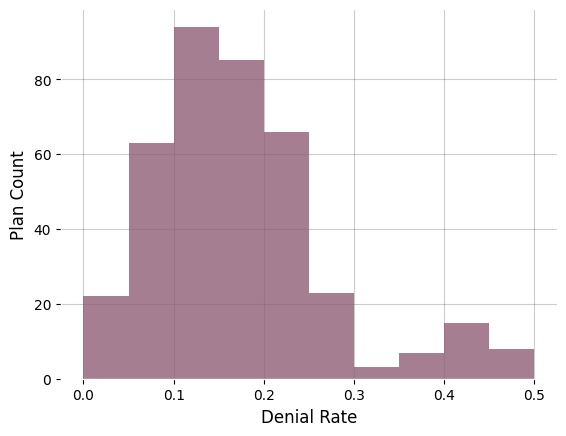
\includegraphics[width=\textwidth]{images/cms_puf/Gold_dist.png}
				\end{subfigure}
				\hfill
				\begin{subfigure}[t]{0.49\textwidth}
					\centering
					\textbf{Platinum}
					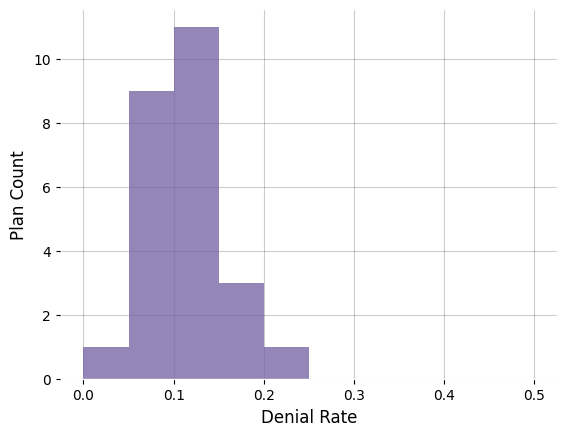
\includegraphics[width=\textwidth]{images/cms_puf/Platinum_dist.png}
				\end{subfigure}

				
				\caption{Distribution of claims denial rates broken down by metal level. From left to right, top to bottom: Catastophic, Bronze, Bronze Expanded, Silver, Gold and Platinum plan distributions.}
				\label{federaldenialratesbymetallevel}
			\end{figure}
		
		
		\clearpage
		
		Figure \ref{federalbyregion} shows the average issuer level claims denial rates for each state or region represented in the CMS TIC PUF data, as well as various statistics of the data within each region. For example, we display the number of issuers represented in each state, the total number of claims represented for each state, and the issuers with the highest claims denial rates in each state.
					
					
		\begin{figure}[h!]
			\centering
			\textbf{Denial Rates By Region}\\
			\textbf{Federal Marketplace, 2021}\\
			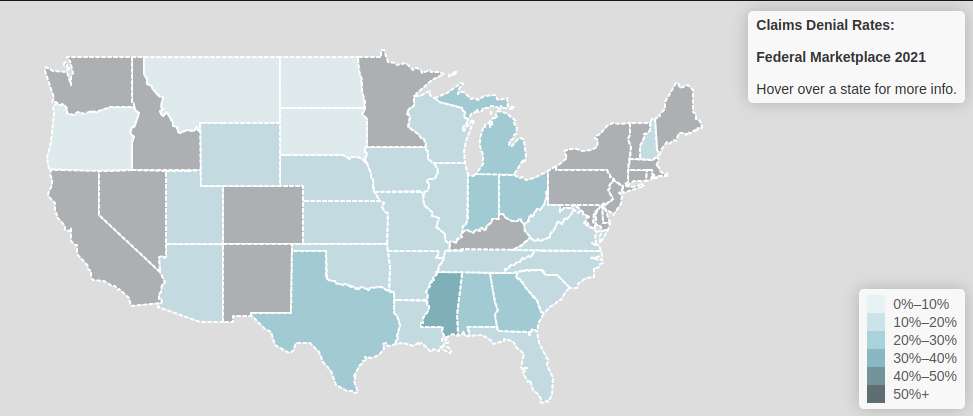
\includegraphics[width=\columnwidth]{images/cms_puf/federal_denial_rates.png}
			\caption{Claims denial rates in the 2021 CMS PUF data broken down by region.}
			\label{federalbyregion}
		\end{figure}
	
		Among this federal marketplace data, Mississippi stands out for having a uniquely high aggregate denial rate, with Texas, Alabama, Alaska, Georgia, Ohio, Indiana and Michigan forming a contingent with the next highest rates.
		
		In many regions, a relatively small collection of issuers contribute a majority of the claims denied.
		
		\underline{New York Health Care Claims Reports}\\
		
		The New York Health Care Claims Reports provide a \emph{different} set of metadata associated with individual insurers, and their corresponding aggregate claims data, that allow denials to be considered from different lenses. The claims reports also include information relating to the monetary value of claims, which we consider in more detail below.
		
		The reports include information that details how claims, denials, and appeals are broken down across different provider categories. The categories specified in the data are:
		
		\begin{itemize}
			\item Hospital Inpatient
			\item Hospital Outpatient
			\item Other Facilities Inpatient
			\item Physicians
			\item Other Health Care Providers
			\item Pharmacy
			\item Other
		\end{itemize}
	
		Of note, the ``Hospital Outpatient'' category includes all claims submitted for emergency room services, and the ``Other Facilities Inpatient'' category includes all claims submitted for inpatient rehabilitation or skilled nursing facility services.
		
		Figure \ref{nyclaimsbyprovidercat} shows the overall claims counts occurring in the dataset for each category, while Figure \ref{nydenialsbyprovidercat} shows the overall claims denial rates in each category, aggregated over all insurers in the dataset.
		
		
		\begin{figure}[h!]
			\centering
			\textbf{Claims By Provider Category}\\
			\textbf{NY, 2022}\\
			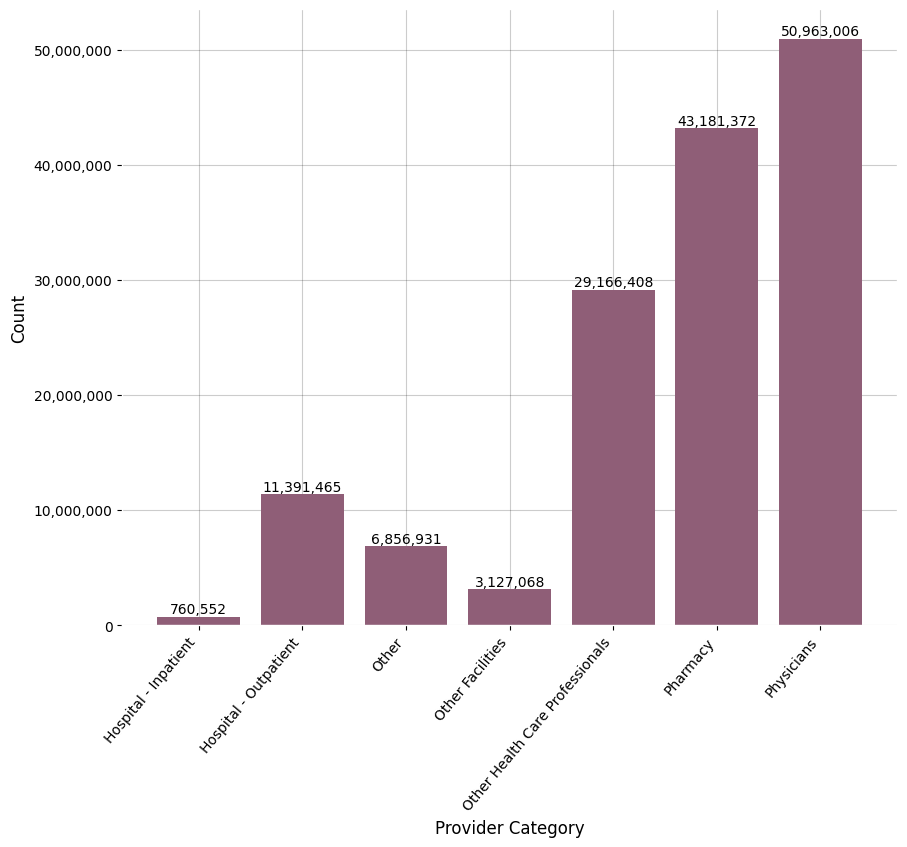
\includegraphics[width=\columnwidth]{images/ny_claim_reports/claims_by_provider_cat.png}
			\caption{ Claims counts broken down by provider category, aggregated across all insurers who submitted health care claims reports to the Department of Financial Services in 2022.}
			\label{nyclaimsbyprovidercat}
		\end{figure}
	
	
		\begin{figure}[h!]
			\centering
			\textbf{Denials By Provider Category}\\
			\textbf{NY, 2022}\\
			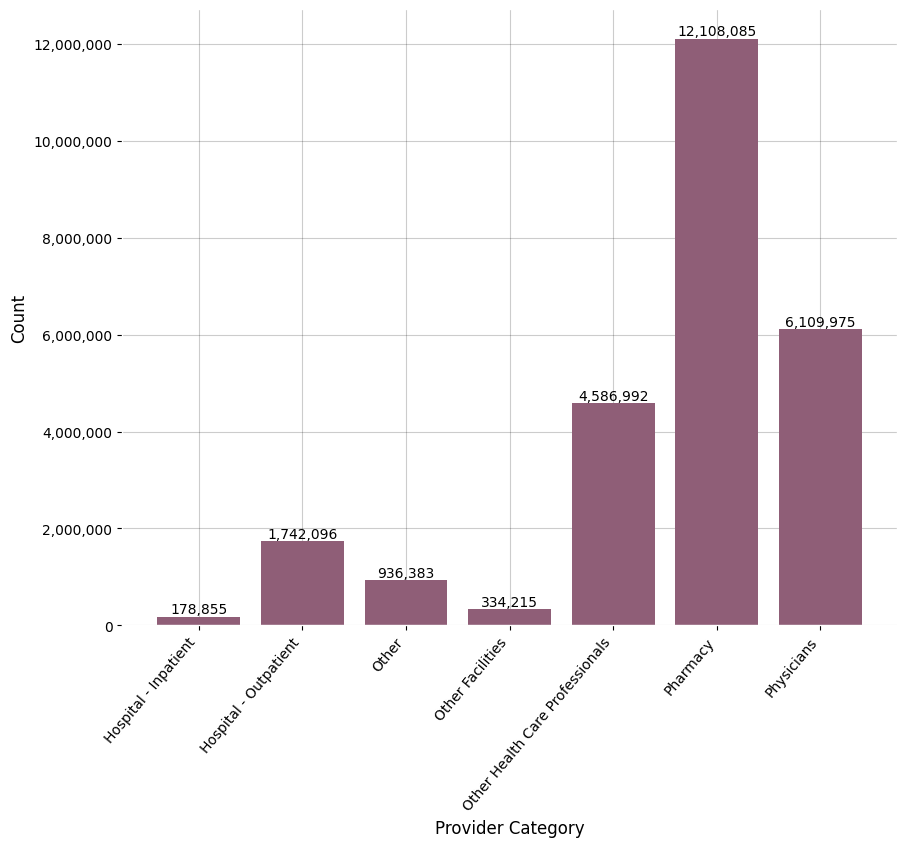
\includegraphics[width=\columnwidth]{images/ny_claim_reports/denials_by_provider_cat.png}
			\caption{Denial counts broken down by provider category, aggregated across all insurers who submitted health care claims reports to the Department of Financial Services in 2022.}
			\label{nydenialsbyprovidercat}
		\end{figure}
	
		\clearpage
	
		The relative frequency of denials across these categories is somewhat consistent with the distribution of claims received across the categories, but denial rates vary from 10\% to 30\% across the categories.
		
		We can also observe how NMN denials specifically are broken down by provider category. This is shown in Figure \ref{nynmndenialsbyprovidercat}.
		
		\begin{figure}[h!]
			\centering
			\textbf{NMN Denials By Provider Category}\\
			\textbf{NY, 2022}\\
			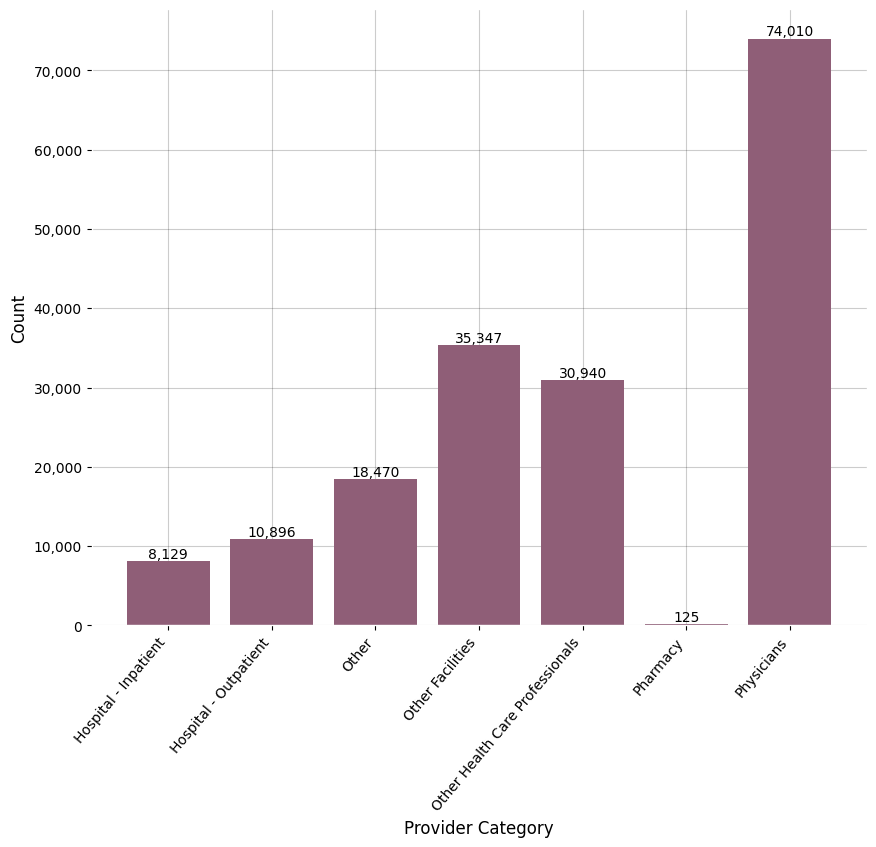
\includegraphics[width=\columnwidth]{images/ny_claim_reports/nmn_denials_by_provider_cat.png}
			\caption{Total claims denied for medical necessity or experimental nature of a treatment, for each provider category, aggregated across all insurers who submitted health care claims reports to the Department of Financial Services in 2022.}
			\label{nynmndenialsbyprovidercat}
		\end{figure}
	
	\clearpage
	
	
		The New York Health Care Claims Reports are unique in that they also provide detailed breakdowns of the monetary value associated with many of the aspects of the data they report. Generally, the data reports the value of claims in various subcategories via two mechanisms:
		
		\begin{itemize}
			\item \emph{Allowed Amounts}
			
				An \href{https://www.healthcare.gov/glossary/allowed-amount/}{allowed amount} for a service under a given plan is the maximum monetary value that the insurance plan will pay for a covered service.
				
			\item \emph{Billed Charges}
			
			A billed charge is the actual monetary value that a service provider charges a patient or insurer; this amount need not agree with the allowed amount for a plan.
			
		\end{itemize}
			
		Figure \ref{nynmnallowedbyprovidercat} shows the collective value of NMN denials in the dataset, as measured by the total allowed amounts. Allowed amounts for NY NMN denials accounted for over 35M USD in 2022.
		
		\begin{figure}[h!]
			\centering
			\textbf{Allowed Amounts for NMN Denials}\\
			\textbf{By Provider Category}\\
			\textbf{NY, 2022}\\
			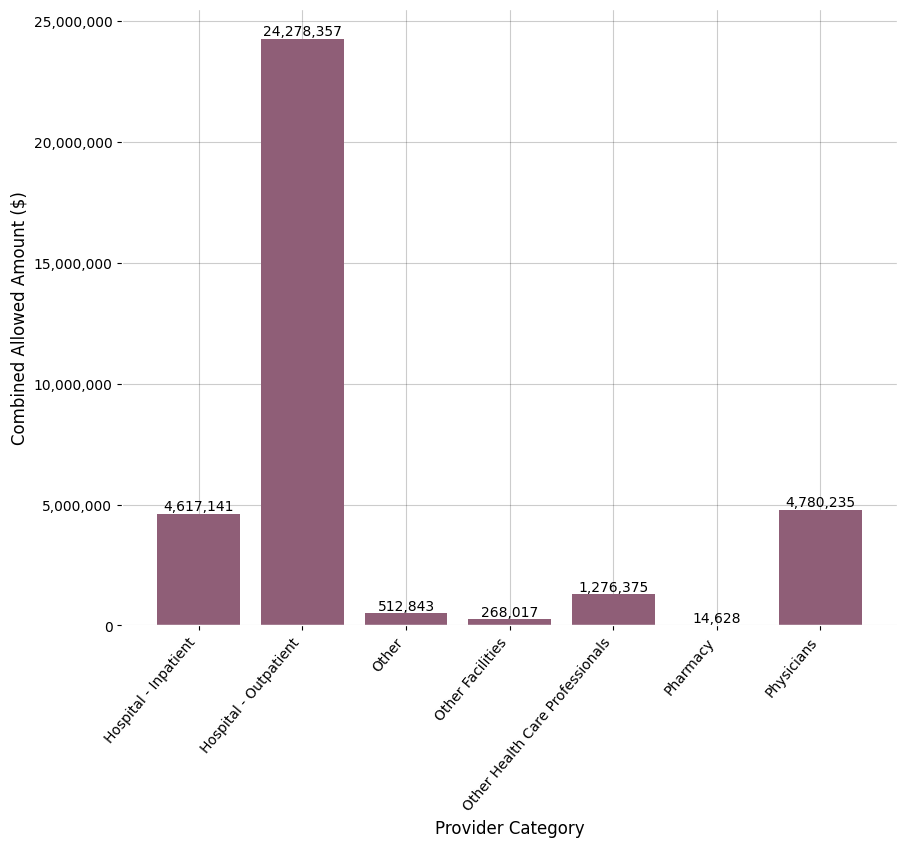
\includegraphics[width=\columnwidth]{images/ny_claim_reports/nmn_allowed_amts_by_provider_cat.png}
			\caption{Total allowed amounts for claims denied for medical necessity or experimental nature of a treatment, for each provider category, aggregated across all insurers who submitted health care claims reports to the Department of Financial Services in 2022.}
			\label{nynmnallowedbyprovidercat}
		\end{figure}
	
		\clearpage
	
		
		The distributions for both NMN denial counts and corresponding allowed amounts across provider categories look largely similar to those for all denials, with two notable exceptions.
		
		\begin{itemize}
			\item There are very few Pharmacy denials for medical necessity in this data. One contributing factor for this is that the NMN category in this data does not include denials requiring the use of step therapy. While this is a separate denial category in this data, the categories are similar in that they involve a determination about purportedly medically appropriate treatments. Another contributing factor to the relative scarcity of pharmacy NMN denials is the reporting methodology: pre-authorization denials are not included in this data, which is one context in which one would expect NMN pharmacy denials to be occurring.
			
			\item Among NMN denials, Hospital Outpatient allowed amounts far outweigh those of Hospital Inpatient, unlike in the distribution among denials of all types.
			
		\end{itemize}
	
	
		While there are likely many factors driving the latter result, it is worth noting that generally \href{https://www2.deloitte.com/us/en/insights/industry/health-care/outpatient-virtual-health-care-trends.html}{data suggests} that hospital revenue share from outpatient procedures has been consistently increasing, with a \href{https://www.mckinsey.com/industries/healthcare/our-insights/walking-out-of-the-hospital-the-continued-rise-of-ambulatory-care-and-how-to-take-advantage-of-it}{large share of orthopedic and minor surgeries} occurring in outpatient settings. Collectively, these trends to perform certain types of services and treatments more frequently in outpatient vs inpatient settings, coupled with the distribution of purported medical necessity of services within these disciplines, as dictated by insurers, might explain why NMN denials for outpatient services correspond to a high total allowed amount, relative to the inpatient NMN denials.
		
		We can also consider the proportion of denials in each provider category that correspond to each denial rationale. Figure \ref{nyrationalesbyprovidercat} shows a heatmap displaying these distributions.
		
		
		\begin{figure}[h!]
			\centering
			\textbf{Denial Rationales By Provider Category}\\
			\textbf{NY, 2022}\\
			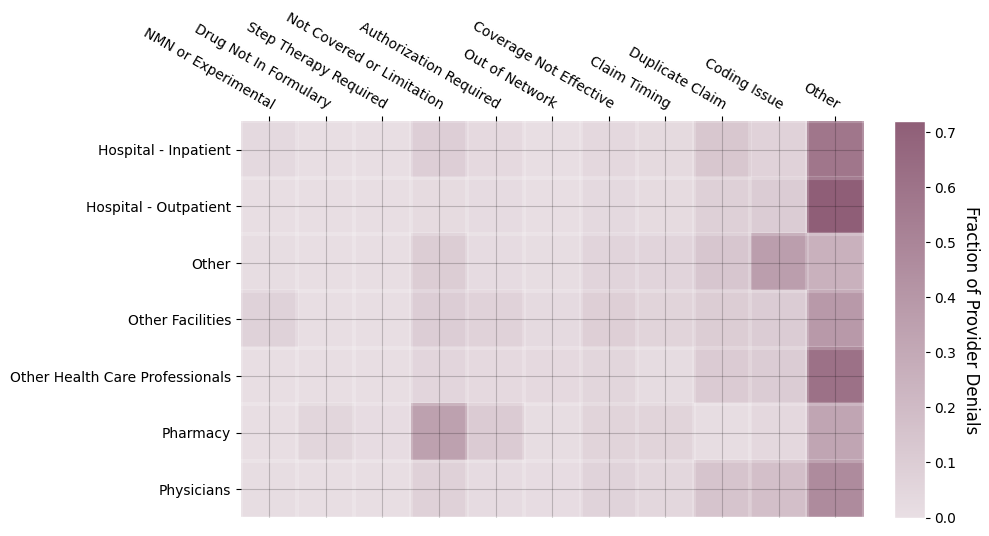
\includegraphics[width=\columnwidth]{images/ny_claim_reports/provider_cat_vs_denial_cat.png}
			\caption{Distribution of denial rationales for each provider category in the 2022 Department of Financial Services claims report data. The color indicates the fraction of all denials in a given provider category that were coded with a particular rationale (i.e. rows sum to 1).}
			\label{nyrationalesbyprovidercat}
		\end{figure}
	
		\clearpage
	
		While it is difficult to extract detail about the distributions from Figure \ref{nyrationalesbyprovidercat} given the prevalence of ``Other'' rationale reporting, some trends are noticeable. For example, among the Pharmacy denials in the dataset that are not recorded under the ``Other'' category, a large proportion are coded as denials related to non-covered or limited services.
		
		
		\underline{Connecticut Consumer Report Cards}\\
		
		The Connecticut Consumer Report Cards provide a few types of information that are not present in the other datasets. Most notably for our purposes, the reports include detailed breakdowns of how claims counts and enrollment are split across different market segments, such as plan type, plan funding type, and insurer. We display a few statistics relating to enrollment in what follows.
		
		All claims data in the consumer report corresponds to a certain population of consumers. Understanding that population is highly relevant, as it serves as an important denominator for considerations about the average impact of claims denials on each person. For example, one might be interested in understanding the average number of medical necessity claims denials received by an individual member of an insurance plan over the course of a year. This sort of calculation requires an understanding of not just raw claims and denial numbers, but also enrollment, associated with a plan.
		
		As we noted previously, the entire dataset corresponds to 1,991,903 insured people. Figure \ref{ctenrollmentbyinsurer} shows how that total enrollment is broken down across the insurers represented in the data.
		
		
		\begin{figure}[h!]
			\centering
			\textbf{Enrollment by Insurer}\\
			\textbf{CT, 2021}\\
			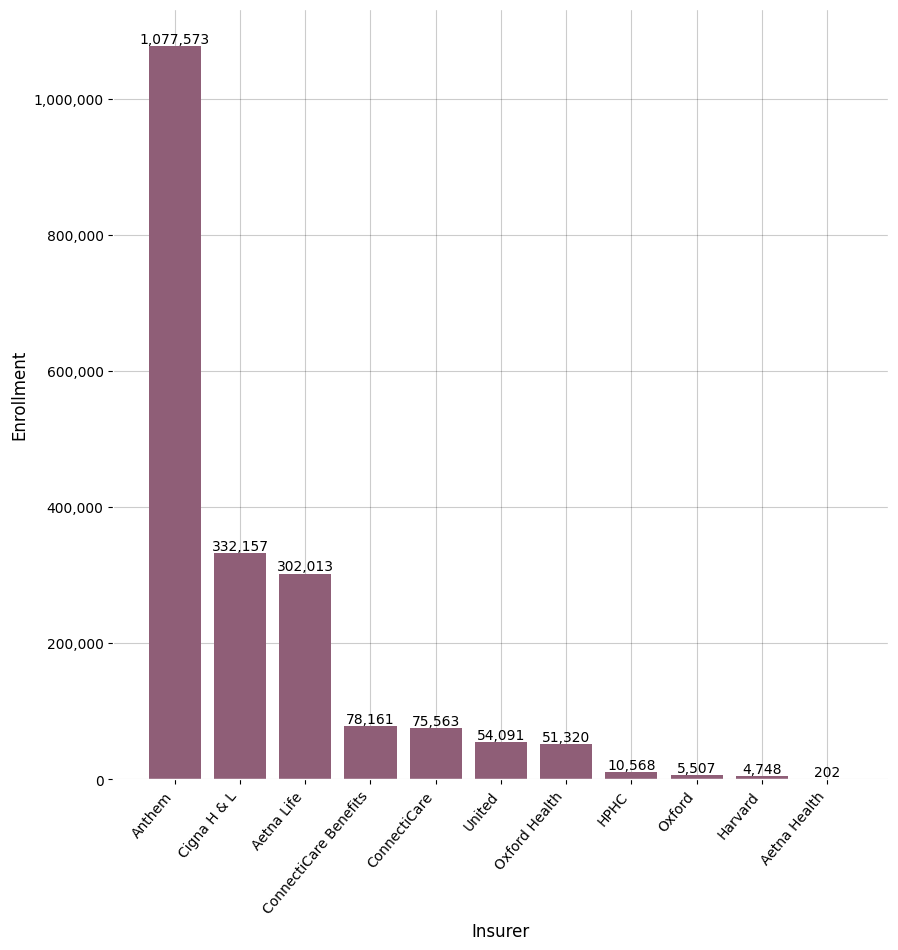
\includegraphics[width=\columnwidth]{images/ct_claims/enrollment_by_insurer.png}
			\caption{Enrollment in CT consumer report card broken down by insurer.}
			\label{ctenrollmentbyinsurer}
		\end{figure}
		\clearpage
	
		Figures \ref{ctenrollmentbygrouptype} and \ref{ctenrollmentbyfundingtype} respectively display how the total enrollment is split across:
		
		\begin{itemize}
			\item \emph{Individual}, \emph{small group}, and \emph{large group} plans
			
			Individual plans are plans purchased on an individual basis, for example through the federal or a state based Affordable Care Act (ACA) marketplace. In the case at hand, this means plans bought through Connecticut's marketplace, \href{https://www.accesshealthct.com}{Access Health Connecticut}. Group plans are plans administered for a group of employees or other beneficiaries; the term \emph{small group} has technical meaning that varies by state, but typically refers to employer group health plans for employers with 50 or fewer employees.
			
			\item \emph{Self insured} and \emph{fully insured} plans
			
			\href{https://www.healthcare.gov/glossary/self-insured-plan/}{Self insured} plans are group plans in which premiums are collected by, and covered services for the insured are paid for by, an employer itself. Such plans need not take on the administrative burden of insurance coverage, and often outsource that aspect of insuring to large, well-known insurance companies (often referred to as third party administrators, or TPMs, when they are employed in this role). \href{https://www.healthcare.gov/glossary/fully-insured-job-based-plan/}{Fully insured} plans are plans purchased by an employer.
		\end{itemize}
	
		\begin{figure}[h!]
			\centering
			\textbf{Enrollment by Group Type}\\
			\textbf{CT, 2021}\\
			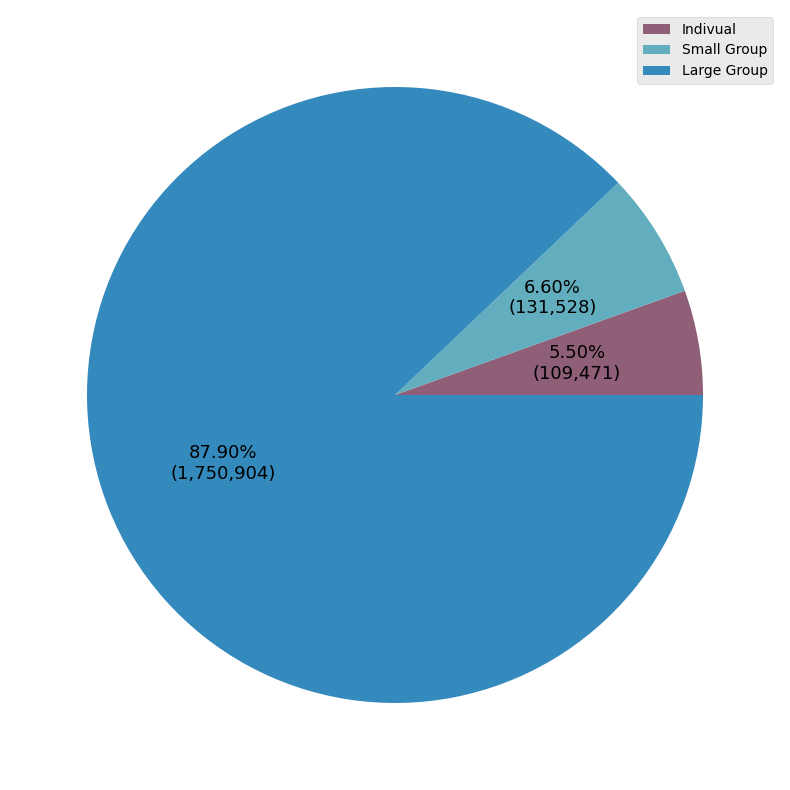
\includegraphics[width=.5\columnwidth]{images/ct_claims/enrollment_by_group_type.png}
			\caption{Enrollment in CT consumer report card broken down by group type. The data are partitioned according to individual, small group, and large group plans.}
			\label{ctenrollmentbygrouptype}
		\end{figure}


		\begin{figure}[h!]
			\centering
			\textbf{Enrollment by Funding Type}\\
			\textbf{CT, 2021}\\
			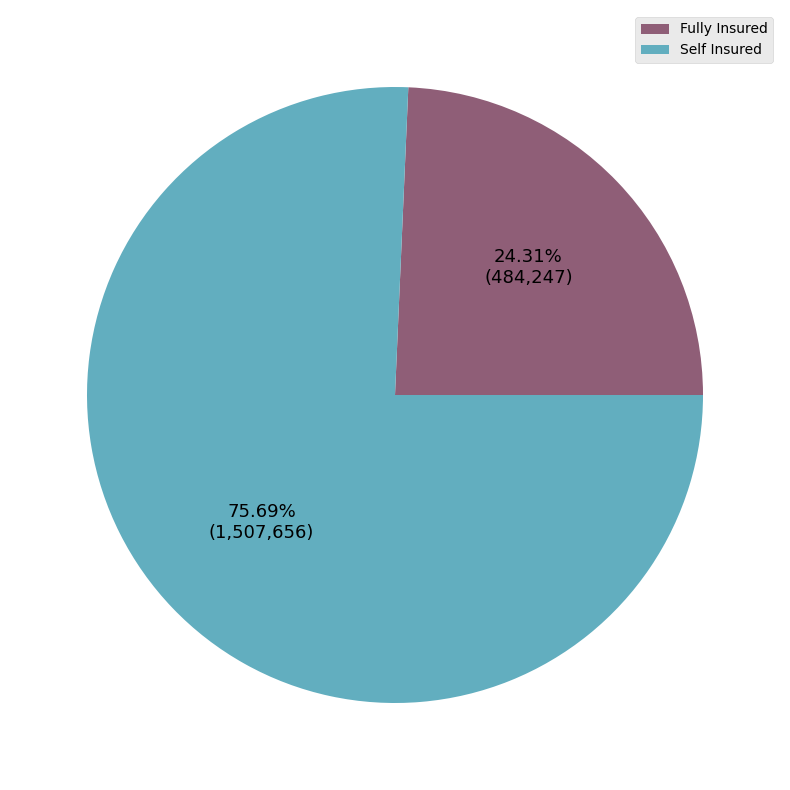
\includegraphics[width=.5\columnwidth]{images/ct_claims/enrollment_by_payer_type.png}
			\caption{Enrollment in CT consumer report card broken down by payer type. The data are partitioned according to fully insured plans and self funded plans.}
			\label{ctenrollmentbyfundingtype}
		\end{figure}
	
		\clearpage
	
		The data from Connecticut is unique in that it includes a large population of large group health plans, which together with the other data provides for a relatively comprehensive view of the total insured population in the state. It would be invaluable to have such comprehensive data for all states.
		
		\subsubsection{Summary of Findings}
		
		In studying claims and denials in each of the datasets considered, we've observed a few key points
		that are consistent across market segments and marketplaces. 
		
		\begin{itemize}
			\item Denials are extremely prevalent, with claims denial rates consistently hovering between 10\% and 30\%.
			\item Reporting standards are insufficient to understand the landscape of denials; most denial rationales are recorded
			as ``Other'', which is inadequate for understanding how and why denial rates vary across insurers, provider categories,
			and other partitions of claims.
			\item Denials pertaining to medical necessity or the experimental nature of treatments comprise a small fraction of
			all denials, but still account for a large absolute pool of claims denials, and money.
		\end{itemize}
		
		Informed by these findings, we discuss some proposals for improving patient outcomes 
		in the \hyperref[recommendations]{recommendations} section below.
		
		
		
		\subsection{Internal Appeals}\label{publicdata:internalappeals}
		
		Next we consider the occurrence of internal appeals in the data. The same datasets that provide information sufficient to compute raw claims denial rates provide information about internal appeals. We again consider these datasets:
		
		\begin{itemize}
			\item CMS TIC PUFs.
			\item New York Health Care Claims Reports.
			\item Connecticut Consumer Report Cards.
			\item Pennsylvania Department of Insurance Data.
		\end{itemize}
	
		Despite the inconsistencies in reporting across the datasets, the data is striking in that it consistently makes clear that while appeals of all forms are extremely rare among consumers, internal appeal overturn rates are high. We note that this disparity between the fraction of denials being internally appealed and the fraction of those appeals being internally overturned could be rooted in various phenomena \footnote{For example, it could be the case that the distribution of cases being internally appealed are those that are particularly egregious, or obviously inappropriate, denials, and that the expected appeal success rate would drop drastically if one were to appeal every denial with the adjudication processes remaining fixed. }.
		
		
		\subsubsection{Overall Internal Appeal Rates}
		
		\underline{CMS Federal Marketplace PUFs}
		
		The CMS PUFs report the number of internal appeals submitted for denied claims only at the issuer level (so there is not enough information to determine the internal appeal rate for a particular plan).
		
		Analyzing this data is more subtle than it ought to be, because not all issuers in the dataset that report their denial counts report their internal appeals counts, and not all issuers that report their internal appeal counts report their external appeal counts. As a result, simply calculating the ratio of the number of internal appeals reported in the data to the number of denials recorded in the data would only give a lower bound on the internal appeal rate. To address this, we report internal appeal rates by restricting attention to those plans that report both denials and internal appeals.
		
		Among 2021 federal marketplace plans, the average initial appeal rate is about .2\%, while the internal appeal overturn rate among this same population of internally appealed claims is about 41\%. This data is shown in Figure \ref{federalinternalappealpie}.
		
	
	
	\begin{figure}[h!]
		\centering
		\begin{subfigure}[b]{0.49\textwidth}
			\centering
			\textbf{Overall Internal Appeal Rate}\\
			\textbf{Federal Marketplace, 2021}\\
			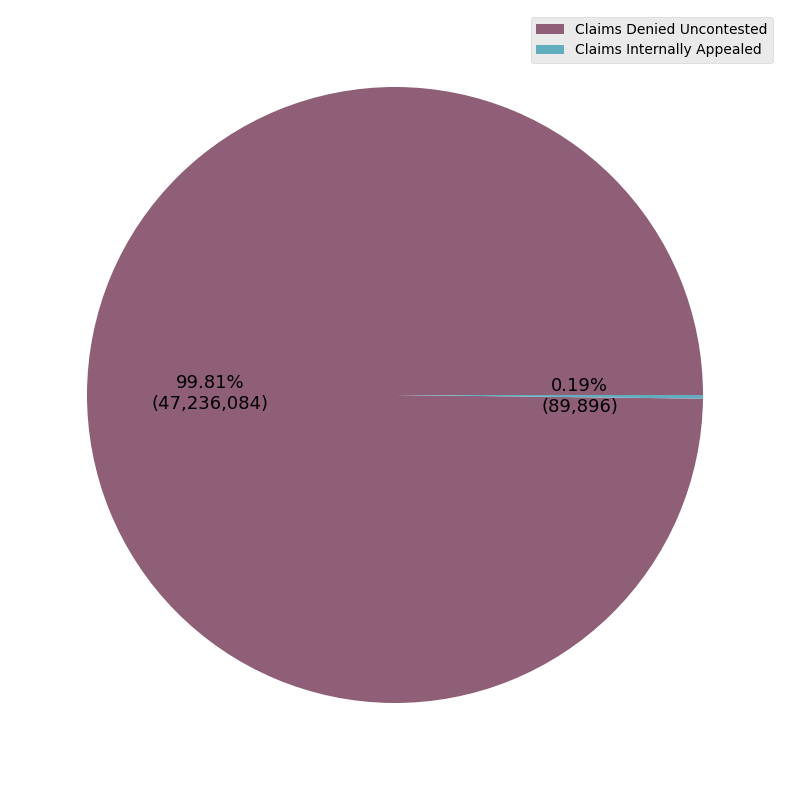
\includegraphics[width=\textwidth]{images/cms_puf/internal_appeal_rates_all_insurers.png}
		\end{subfigure}
		\hfill
		\begin{subfigure}[b]{0.49\textwidth}
			\centering
			\textbf{Overall Internal Appeal Overturn Rate}\\
			\textbf{Federal Marketplace, 2021}\\
			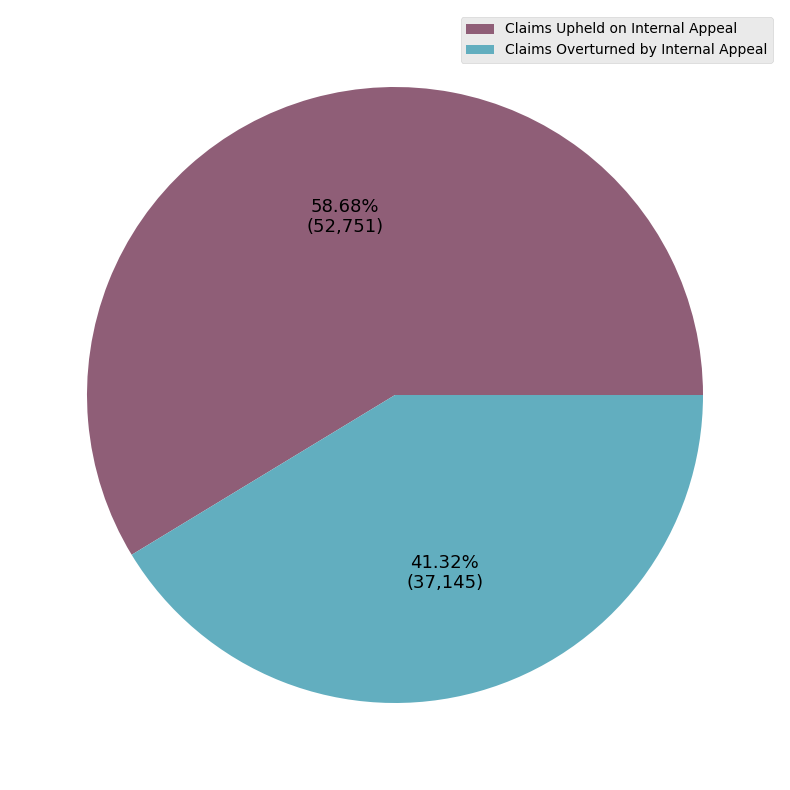
\includegraphics[width=\textwidth]{images/cms_puf/internal_appeal_success_rates_all_insurers.png}
		\end{subfigure}
		\caption{Internal appeal rates and appeal overturn rates among federal marketplace issuers in 2021. Only 1/5 of a percent of the approximately 48 million initially denied claims are appealed, but of those that are, 41 percent get overturned on a first level internal review.}
		\label{federalinternalappealpie}
	\end{figure}
	
		\clearpage
	
		\underline{New York Health Care Claims Reports}
		
		The New York Health Care Claims Reports document the number of internal appeals submitted for each insurer in the data. Figure \ref{nyinternalappealpie} shows the fraction of all initially denied claims that are internally appealed by consumers, and the fraction of those that are overturned on initial appeal. The initial appeal rate is about .6\%, while the internal appeal overturn rate among these claims is about 29\%.
		
		
		\begin{figure}[h!]
			\centering
			\begin{subfigure}[b]{0.49\textwidth}
				\centering
				\textbf{Overall Internal Appeal Rate}\\
				\textbf{NY, 2022}\\
				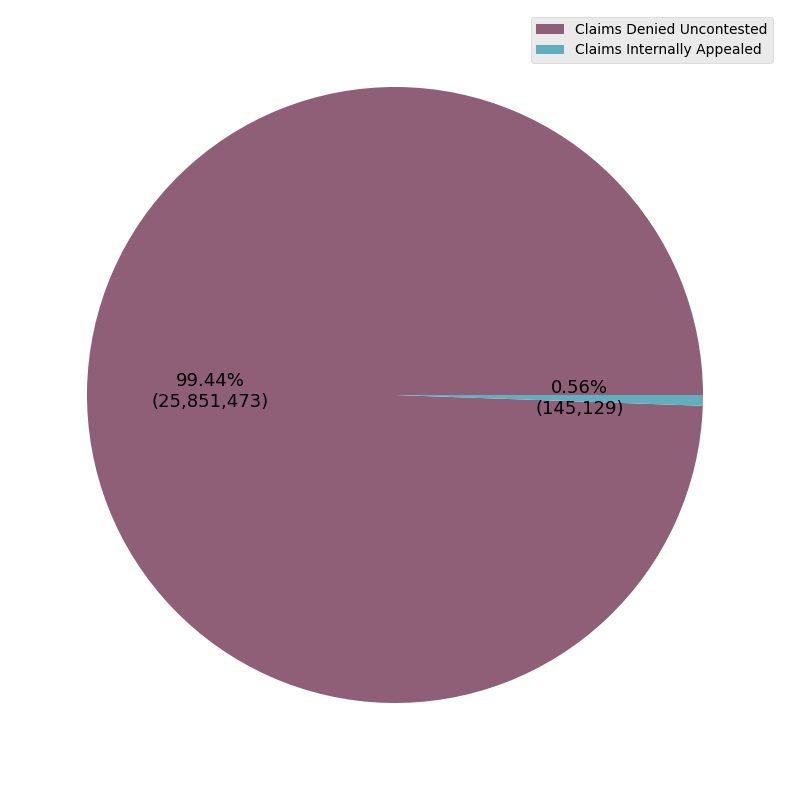
\includegraphics[width=\textwidth]{images/ny_claim_reports/internal_appeal_pie.png}
			\end{subfigure}
			\hfill
			\begin{subfigure}[b]{0.49\textwidth}
				\centering
				\textbf{Overall Internal Appeal Overturn Rate}\\
				\textbf{NY, 2022}\\
				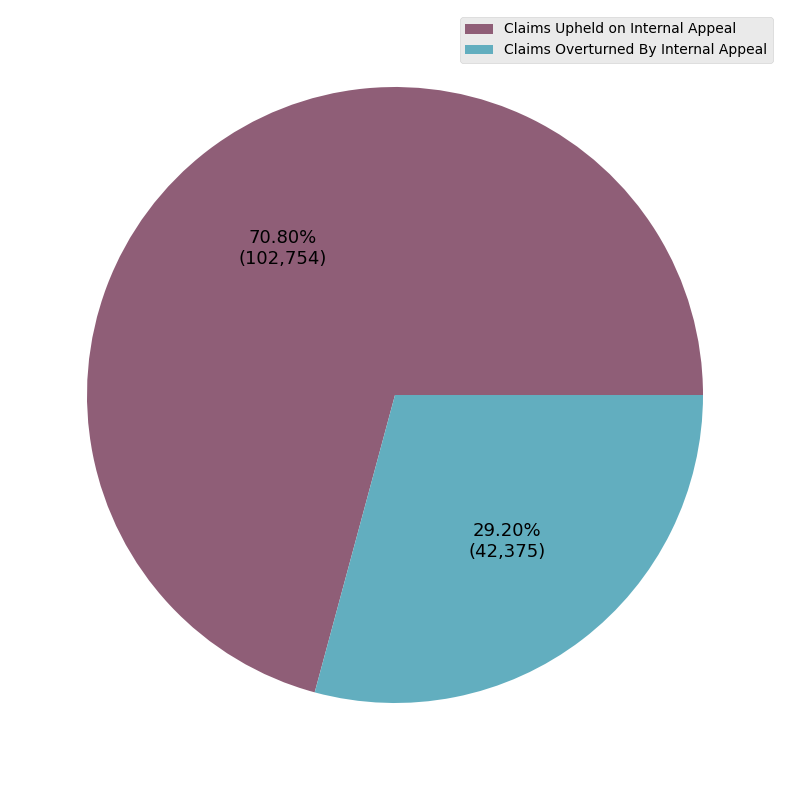
\includegraphics[width=\textwidth]{images/ny_claim_reports/internal_appeal_overturns_pie.png}
			\end{subfigure}
			\caption{Internal appeal rates and appeal overturn rates among insurers who submitted health care claims reports to the Department of Financial Services in 2022. Only 1/2 of a percent of the approximately 25 million initially denied claims are appealed, but of those that are, 29 percent get overturned on a first level internal review.}
			\label{nyinternalappealpie}
		\end{figure}
	
		\underline{Connecticut Consumer Report Cards}
		
		The Connecticut Consumer Report Cards document the number of internal appeals submitted for each insurer in the data. Figure \ref{ctinternalappealpie} shows the fraction of all initially denied claims that are internally appealed by consumers, and the fraction of those that are overturned on initial appeal. The initial appeal rate is about .4\%, while the internal appeal overturn rate among these claims is about 60\%.
		
		
		\begin{figure}[h!]
			\centering
			\begin{subfigure}[b]{0.49\textwidth}
				\centering
				\textbf{Overall Internal Appeal Rate}\\
				\textbf{CT, 2021}\\
				\includegraphics[width=\textwidth]{images/ct_claims/internal_appeal_rates_all_insurers.png}
			\end{subfigure}
			\hfill
			\begin{subfigure}[b]{0.49\textwidth}
				\centering
				\textbf{Overall Internal Appeal Overturn Rate}\\
				\textbf{CT, 2021}\\
				\includegraphics[width=\textwidth]{images/ct_claims/internal_appeal_success_rates_all_insurers.png}
			\end{subfigure}
			\caption{Overall internal appeal rates in the CT consumer report card data. Only .4 percent of the approximately 2 million initially denied claims are appealed, but of those that are, 60 percent get overturned on a first level internal review.}
			\label{ctinternalappealpie}
		\end{figure}
		
		
		\underline{Pennsylvania Department of Insurance Data}
		
		
		Figure \ref{painternalappealpie} shows the fraction of all initially denied claims that are internally appealed by consumers, and the fraction of those that are overturned on initial appeal in the 2020 and 2021 PA DOI data. The initial appeal rate is about .1\%, while the internal appeal overturn rate among these claims is about 59\%.
		
		\begin{figure}[h!]
			\centering
			\begin{subfigure}[b]{0.49\textwidth}
				\centering
				\textbf{Overall Internal Appeal Rate}\\
				\textbf{PA, 2020-2021}\\
				\includegraphics[width=\textwidth]{images/pa_claims/internal_appeal_pie.png}
			\end{subfigure}
			\hfill
			\begin{subfigure}[b]{0.49\textwidth}
				\centering
				\textbf{Overall Internal Appeal Overturn Rate}\\
				\textbf{PA, 2020-2021}\\
				\includegraphics[width=\textwidth]{images/pa_claims/internal_appeal_overturns_pie.png}
			\end{subfigure}
			\caption{Overall internal appeal rates in the PA DOI data. Only .1 percent of the approximately 3 million initially denied claims are appealed, but of those that are, 59 percent get overturned on a first level internal review.}
			\label{painternalappealpie}
		\end{figure}
	
	\clearpage
		
				
		
		\subsubsection{Internal Appeals By Insurer}
		
		As we noted above, each of the datasets provides enough information to compute appeal rates and appeal overturn rates on an individual insurer basis. In what follows we share some such calculations.
		
		\underline{CMS Federal Marketplace PUFs}
		
		Figures \ref{federalinternalappealratebyinsurer} and \ref{federalinternalappealoverturnratebyinsurer} show the internal appeal rates and internal appeal overturn rates for the 10 insurers with the largest volume of claims adjudicated in the 2021 CMS PUF data.
		
		
		\begin{figure}[h!]
			\centering
			\textbf{Internal Appeal Rate By Insurer}\\
			\textbf{Federal Marketplace, 2021}\\
			\includegraphics[width=.8\columnwidth]{images/cms_puf/internal_appeal_rate_by_insurer.png}
			\caption{Internal appeal rates for the 10 insurers with the largest number of claims adjudicated in the 2021 federal marketplace data.}
			\label{federalinternalappealratebyinsurer}
		\end{figure}
	
	
		\begin{figure}[h!]
			\centering
			\textbf{Internal Appeal Overturn Rate By Insurer}\\
			\textbf{Federal Marketplace, 2021}\\
			\includegraphics[width=.8\columnwidth]{images/cms_puf/internal_appeal_overturn_rate_by_insurer.png}
			\caption{Internal appeal overturn rates for the 10 issuers with the largest number of claims adjudicated in the 2021 federal marketplace data.}
			\label{federalinternalappealoverturnratebyinsurer}
		\end{figure}
	
		\clearpage
		
		\underline{New York Health Care Claims Reports}
		
		Figures \ref{nyinternalappealratebyinsurer} and \ref{nyinternalappealoverturnratebyinsurer} show the internal appeal rates and internal appeal overturn rates for the 10 insurers with the largest volume of claims adjudicated in the NY claims report data.
		
		\begin{figure}[h!]
			\centering
			\textbf{Internal Appeal Rate By Insurer}\\ 
			\textbf{NY, 2022}\\
			\includegraphics[width=.8\columnwidth]{images/ny_claim_reports/appeal_rate_by_insurer.png}
			\caption{ Internal appeal rates for the 10 insurers with the largest number of claims adjudicated in the 2022 Department of Financial Services claims report data.}
			\label{nyinternalappealratebyinsurer}
		\end{figure}
		
		
		\begin{figure}[h!]
			\centering
			\textbf{Internal Appeal Overturn Rate By Insurer}\\
			\textbf{NY, 2022}\\
			\includegraphics[width=.8\columnwidth]{images/ny_claim_reports/internal_appeal_overturn_rate_by_insurer.png}
			\caption{Internal appeal overturn rates for the 10 insurers with the largest number of claims adjudicated in the 2022 Department of Financial Services claims report data.}
			\label{nyinternalappealoverturnratebyinsurer}
		\end{figure}
		
		\clearpage
		
		
		\underline{Connecticut Consumer Report Cards}

		Figures \ref{ctinternalappealratebyinsurer} and \ref{ctinternalappealoverturnratebyinsurer} show the internal appeal rates and internal appeal overturn rates for all insurers in the Connecticut consumer report card data.
		
		\begin{figure}[h!]
			\centering
			\textbf{Internal Appeal Rate By Insurer}\\
			\textbf{CT, 2021}\\
			\includegraphics[width=.8\columnwidth]{images/ct_claims/appeal_rate_by_insurer.png}
			\caption{Internal appeal rates for insurers in the 2022 Connecticut Consumer Report Card Data.}
			\label{ctinternalappealratebyinsurer}
		\end{figure}
		
		
		\begin{figure}[h!]
			\centering
			\textbf{Internal Appeal Overturn Rate By Insurer}\\
			\textbf{CT, 2021}\\
			\includegraphics[width=.8\columnwidth]{images/ct_claims/internal_appeal_overturn_rate_by_insurer.png}
			\caption{Internal appeal overturn rates for issuers in the 2022 Connecticut Consumer Report Card Data.}
			\label{ctinternalappealoverturnratebyinsurer}
		\end{figure}
		
		\clearpage
		
		
		\underline{Pennsylvania Department of Insurance Data}

		Figures \ref{painternalappealratebyinsurer} and \ref{painternalappealoverturnratebyinsurer} show the internal appeal rates and internal appeal overturn rates for all insurers in the Pennsylvania Department of Insurance data.
		
		\begin{figure}[h!]
			\centering
			\textbf{Internal Appeal Rate By Insurer}\\
			\textbf{PA, 2020-2021}\\
			\includegraphics[width=.8\columnwidth]{images/pa_claims/appeal_rate_by_insurer.png}
			\caption{Internal appeal rates for 10 insurers with the most claims in the PA DOI data.}
			\label{painternalappealratebyinsurer}
		\end{figure}
		
		
		\begin{figure}[h!]
			\centering
			\textbf{Internal Appeal Overturn Rate By Insurer}\\
			\textbf{PA, 2020-2021}\\
			\includegraphics[width=.8\columnwidth]{images/pa_claims/internal_appeal_overturn_rate_by_insurer.png}
			\caption{Internal appeal overturn rates for 10 insurers with the most claims in the PA DOI data.}
			\label{painternalappealoverturnratebyinsurer}
		\end{figure}
		
		\clearpage
		
		\subsubsection{Dataset Specific Considerations}
		
		The considerations above exhaust most of the analysis on internal appeals that can be done in a common way across the datasets reporting internal appeal counts. In what follows, we consider a few additional aspects of the data reported in only \emph{some} of the datasets.
		
		\underline{New York Health Care Claims Reports}
		
		The data recorded in the New York Health Care Claims Reports allow us to investigate how internal appeal rates and internal appeal overturn rates vary by provider category. Figure \ref{nyappealratesbyprovidercat} shows the overall claims denial rates, internal appeal rates, and internal appeal overturn rates for each of these categories, aggregated over all insurers in the dataset.
		
		\begin{figure}[h!]
			\centering
			\textbf{Denial and Appeal Rates By Provider Category}\\
			\textbf{NY, 2022}\\
			\includegraphics[width=\columnwidth]{images/ny_claim_reports/denial_and_appeal_rates_by_provider_cat.png}
			\caption{Denial, internal appeal, and internal appeal overturn rates across provider categories in the 2022 New York Health Care Claims Reports.}
			\label{nyappealratesbyprovidercat}
		\end{figure}
	
		While all provider categories have relatively high internal appeal overturn rates, initial denial rates and internal appeal rates vary widely across the categories. It is noteworthy that while claims for inpatient hospital visits occupy a small fraction of the total claims covered in the dataset (compare Figure \ref{nyclaimsbyprovidercat}), denial rates for those claims are high at 24\%, and internal appeal rates are two to six times larger than those occurring among the other categories. Despite this increased appeal rate, appeal overturn rates remain high at 27\%.
		
		This empirical phenomenon is informed by considering the underlying costs associated with the claims in each of these provider categories. The cost data, displayed in Figure \ref{nyappealsallowedamts}, shows that the sum of the \emph{allowed amounts} for internally appealed `Inpatient Hospital' claims is greater than the sum for any other category. Moreover, consumers collectively recouped roughly 60\% of the entire monetary value of these appealed `Inpatient Hospital' claims, despite having an appeal overturn rate of only 27\%.
		
		\begin{figure}[h!]
			\centering
			\textbf{Allowed Amounts for Internally}\\
			\textbf{Appealed Claims By Provider Category}\\ 
			\textbf{NY, 2022}\\
			\includegraphics[width=\columnwidth]{images/ny_claim_reports/allowed_amts_by_provider_category_stacked.png}
			\caption{Reported total allowed amounts for internally appealed claims, and appeal overturns, broken down by provider category in the 2022 New York Health Care Claims Reports.}
			\label{nyappealsallowedamts}
		\end{figure}
	
		To summarize, consumer behavior in successfully appealing Hospital Inpatient denials led to the overturn of a very \emph{lucrative} portion of the internally appealed denials in the dataset; this is a fact that is not visible when solely considering denial or appeal rates, but it is consistent with the intuition that the most expensive contractually inappropriate denials are the ones most likely to be appealed by consumers or their providers.
		
		Another contributing factor that may be driving this phenomenon is that hospitals often have significant resources provisioned to address contractually inappropriate denials. Hospitals routinely have departments dedicated to insurance claims resolution, and pay full time staff to navigate claims submission and appeals pertaining to a wide variety of issues. It is natural to expect that professionals with ample experience navigating appeals, working for organizations whose revenue and patients depend on successful claims resolution, would both appeal more frequently than would individual consumers, and fare better in their appeal overturn rates.
		
		\underline{Connecticut Consumer Report Cards}
		
		The data recorded in the Connecticut Consumer Report Cards allows one to consider internal appeal rates and internal appeal overturn rates broken down by the rationale provided for the initial denial. This is an incredibly useful lens through which to view the data, and one which is unfortunately unsupported by most of the datasets.
		
		Figures \ref{ctinternalappealratebydenialrationale} and \ref{ctinternalappealoverturnratebydenialrationale} show the internal appeal rates and internal appeal overturn rates for each denial rationale in the dataset.
		
		
			\begin{figure}[h!]
				\centering
				\textbf{Internal Appeal Rate By Denial Rationale}\\
				\textbf{CT, 2021}\\
				\includegraphics[width=\columnwidth]{images/ct_claims/internal_appeals_by_rationale.png}
				\caption{ Internal appeal rate among the population of claims corresponding to each denial rationale in the 2022 Connecticut Consumer Report Card.}
				\label{ctinternalappealratebydenialrationale}
			\end{figure}

	
	
			\begin{figure}[h!]
				\centering
				\textbf{Internal Appeal Overturn Rate By Denial Rationale}\\
				\textbf{CT, 2021}\\
				\includegraphics[width=\columnwidth]{images/ct_claims/internal_appeal_overturns_by_rationale.png}
				\caption{Internal appeal overturn rate among the population of claims corresponding to each denial rationale in the 2022 Connecticut Consumer Report Card.}
				\label{ctinternalappealoverturnratebydenialrationale}
			\end{figure}
		
		In this dataset, the internal appeal rate for NMN denials is between 10 to 50 times larger than the appeal rates in all other categories. On the other hand, internal appeal \emph{overturn} rates for internally appealed NMN denials are among the lowest of all categories.
		
		
		We note that the high rate of internal appeals for denials whose rationales involve medical necessity, or the purported experimental nature of a treatment or service, has an intuitive potential cause. Medical necessity of particular services or care is not typically made explicit in insurance contracts; instead, broad definitions, which themselves reference literature and other documents, dictate a purported standard by which medical necessity will be determined. Given these definitions are often ambiguous and ill-defined in nature, it makes good sense that cases involving them would be more subtle, and be more likely to be appealed, than clear cut cases.
		
		
		For example, if a contract explicitly states something is not covered, or a claim is inappropriately submitted and then denied for a member whose coverage had lapsed at the date of service, there is not much ground on which to make an appeal. This same logic explains why the internal appeal overturn rate is 100\% for internally appealed claims which were denied purportedly because they were duplicates; whether or not a claim is a duplicate is a clear cut matter of accounting, so any substantiated appeal of a claim denied for being purportedly duplicate is likely to be sound.
		
		\subsubsection{Summary of Findings}
		
		In studying internal appeals in each of the datasets considered, we've observed a few key points
		that are consistent across market segments and marketplaces. 
		
		\begin{itemize}
			\item While claims denials occur frequently, internal appeal rates are vanishingly low; this fact remains true
			across all categories of denial, so far as can be told from the data which reports sufficient detail
			to make such a determination.
			\item Among internally appealed claims denials overturn rates are high.
			\item The monetary value historically recouped in the observed data through internal appeals overturns
			is large, despite the fact that internal appeals are vanishingly rare.
		\end{itemize}
	
		Informed by these findings, we discuss some proposals for improving patient outcomes 
		in the \hyperref[recommendations]{recommendations} section below.
		
		
		\subsection{External Appeals}\label{publicdata:externalappeals}
		
		We now turn to external appeals. The datasets that provide information relating to external appeals are:
		
		\begin{itemize}
			\item CMS TIC PUFs.
			\item California CDI external appeal database.
			\item California DMHC external appeal database.
			\item New York external appeal database.
			\item Washington external appeal database.
			\item Pennsylvania Department of Insurance data.
		\end{itemize}
	
		Each of these datasets reports metadata relating to external or independent review of denied claims in a different way. Despite the variations in how the data is reported, the independent sources display at least one consistent result: the population of claims denials which are upheld on internal appeal and then externally appealed are overturned by external review boards at high rates. This is a key fact to take away from these datasets.
		
		
		This result suggests that internal review processes may not be sufficient for fair or equitable adjudication. If the populations of internal and external reviewers were all perfectly impartial, and shared consistent, \emph{repeatable} processes for making their determinations, one would expect near perfect agreement between determinations made by the two bodies for the same pool of denied claims.
		
		Instead, we see \emph{staggering disagreement} in each dataset about which of the \emph{externally} appealed claims merit overturn. The disagreement cannot conclusively be attributed to faulty or biased internal appeal processes, but it suggests that either internal appeal adjudication is faulty, external appeal adjudication is faulty, or appeal adjudication is too complex to expect a high degree of consistency between any two reviewers, at least for the population of externally appealed claims. The latter explanation appears unlikely given the relatively consistent external overturn rates across all of the different data sources we exhibit, and across many different independent, third party review organizations.
		
		We note explicitly that it is possible that if one were to submit all internally appealed claims to third party external review organizations, one would find that \emph{among the population of internally appealed claims} there would be a high degree of agreement between internal and external reviewers on appropriate determination outcomes. It is of course impossible to surmise what this hypothetical level of agreement would be if the audit were to occur.
		
		However, note that even if this \emph{hypothetical} test were to result in overwhelming agreement between internal and external reviewers when considering the population of internally appealed claims, such a result would not negate the problematic nature of the \emph{actual} level of disagreement between internal and external reviewers when considering externally appealed claims denials alone. There is no reason to believe that the population of internally and externally appealed claims are drawn from similar distributions, and as the data clearly shows, the population of internally appealed claims is orders of magnitude larger.
		
		It appears that internal processes may effectively be hoops through which consumers must jump before they are afforded unbiased consideration of their appeals. In fact, historically, most consumers that have navigated their way through an internal appeal process and lost do not (or cannot) proceed with an independent external review, as we will see in the data below.
		
		\subsubsection{Overall External Appeal Rates}
		
		We begin be examining the overall external appeal \emph{overturn} rate in each of the datasets.
		
		The CMS PUF TIC files and PA Department of Insurance data are unique among the external appeals data in that they also allow us to calculate the overall external appeal rates themselves. We calculate this as the total number of external appeals in the dataset divided by the \emph{corresponding} \footnote{Here the word corresponding plays an important role; in some of the datasets, such as the CMS PUFs, not all plans that include internal appeal statistics provide external appeal statistics. As as a result, simply dividing the total number of external appeals by the total number of upheld internal appeals in the dataset would not provide a true measure of an external appeal rate. The denominator would be inaccurately inflated.} total number of upheld internal appeals in the dataset.
		
		All of the other datasets with external appeals data provide information related to submitted external appeals, but do not indicate the corresponding population of upheld internal appeals to which the external appeals correspond. For this reason, we cannot provide an accurate overall external appeal rate in these cases, and instead restrict attention to the overall external appeal overturn rate.
		
		\underline{CMS Federal Marketplace PUFs}
		
		In Figure \ref{federalexternalappealpie}, we display the overall external appeal rate and external appeal overturn rate from the CMS TIC PUF data.
		
		\begin{figure}[h!]
			\centering
			\begin{subfigure}[b]{0.49\textwidth}
				\centering
				\textbf{External Appeal Rate}\\
				\textbf{Federal Marketplace, 2021}\\
				\includegraphics[width=\textwidth]{images/cms_puf/external_appeal_rates_all_insurers.png}
			\end{subfigure}
			\hfill
			\begin{subfigure}[b]{0.49\textwidth}
				\centering
				\textbf{External Appeal Overturn Rate}\\
				\textbf{Federal Marketplace, 2021}\\
				\includegraphics[width=\textwidth]{images/cms_puf/external_appeal_success_rates.png}
			\end{subfigure}
			\caption{Overall external appeal rate and overall appeal overturn rate among federal marketplace issuers that reported the data in 2021. Not all issuers and plans reported external appeal data in the CMS PUF. Among the issuers reporting external appeal data, only 5 percent of the approximately 34 thousand denials upheld on internal appeal are externally appealed, but of those, nearly 49 percent get overturned when reviewed by an independent external agency.}
			\label{federalexternalappealpie}
		\end{figure}
		
		
		Of the 1,760 claims represented in this data that were denied, internally appealed and upheld as denials, and then finally externally appealed, a staggering 49\% were deemed by external reviewers to merit overturn. However, 95\% of the consumers who had their internal appeals of claims denials upheld on internal review did not proceed with the external review process.
		
		\underline{California CDI External Appeal Database}
		
		Figure \ref{cacdiexternalappealpie} shows the overall external appeal overturn rate over the time period covered by the CDI external appeal dataset, excluding data from 2023.
		
		
		\begin{figure}[h!]
			\centering
			\textbf{External Appeal Overturn Rate}\\
			\textbf{CA, CDI Administered, 2011-2022}\\
			\includegraphics[width=.4\textwidth]{images/ca_doi_external_appeals/external_appeal_success_rates.png}
			\caption{External appeal overturn rates among California insurers from 2011 to 2022. Roughly 50 percent of denials that are externally appealed get completely overturned when reviewed by an independent external agency.}
			\label{cacdiexternalappealpie}
		\end{figure}
	
		\clearpage
	
	
		\underline{California DMHC External Appeal Database}

		Figure \ref{cadmhcexternalappealpie} shows the overall external appeal overturn rate over the time period covered by the CDI external appeal dataset, excluding data from 2023.
		
		
		\begin{figure}[h!]
			\centering
			\textbf{External Appeal Overturn Rate}\\
			\textbf{CA, DMHC Administered, 2001-2022}\\
			\includegraphics[width=.4\textwidth]{images/ca_dmhc_external_appeals/external_appeal_success_rates.png}
			\caption{External appeal overturn rates among California issuers from 2001 to 2022. Roughly 49 percent of denials that are externally appealed get completely overturned when reviewed by an independent external agency.}
			\label{cadmhcexternalappealpie}
		\end{figure}
	
		\clearpage
	
		We again see roughly 50\% disagreement between external reviewers and prior internal review determinations among the population of internally upheld and externally appealed claims denials.
		
		\underline{New York External Appeal Database}
		
		Figure \ref{nyexternalappealpie} shows the overall external appeal overturn rate over the time span covered by the New York external appeal dataset, excluding data from 2023.
		
		
		\begin{figure}[h!]
			\centering
			\textbf{External Appeal Overturn Rate}\\
			\textbf{NY, 2022}\\
			\includegraphics[width=.4\textwidth]{images/nys_external/external_appeal_success_rates.png}
			\caption{External appeal overturn rates among New York issuers from 2019 to 2022. Roughly 43 percent of denials that are externally appealed get completely overturned when reviewed by an independent external agency.}
			\label{nyexternalappealpie}
		\end{figure}
	
		\clearpage
		
		In this case, 43\% of internally upheld and externally appealed claims denials are deemed to merit overturn by external reviewers.
		
		We note that while one could attempt to create an estimate for the external appeal rate in NY by combining the upheld internal appeal counts from the health care claims reports, or other sources, with the external appeal counts in this dataset, there is insufficient publicly available information to ensure the underlying population of claims in the two datasets is the same. As a result, even the rough accuracy of such an estimate would be unclear.
		
		\underline{Washington External Appeal Database}
		
		Figure \ref{waexternalappealpie} shows the overall external appeal overturn rate over the time period covered by the Washington external appeal dataset, excluding data from 2023.
		
		
		\begin{figure}[h!]
			\centering
			\textbf{External Appeal Overturn Rate}\\
			\textbf{WA, 2016-2022}\\\
			\includegraphics[width=.4\textwidth]{images/wa_external_appeals/external_appeal_success_rates.png}
			\caption{External appeal overturn rates among OIC regulated Washington health plans from 2016 to 2022. Roughly 25 percent of denials that are externally appealed get completely overturned when reviewed by an independent external agency.}
			\label{waexternalappealpie}
		\end{figure}
	
		\clearpage
	
		At 25\%, the Washington data shows a substantially lower fraction of internally upheld and externally appealed claims denials that are deemed to merit overturn by external reviewers, as compared to the other datasets. This could be influenced by numerous factors, but one possible explanation is that internal appeal review processes are more consistent with external appeal review processes than they are in other states.
		
		\underline{Pennsylvania Department of Insurance Data}
		
		In Figure \ref{paexternalappealpie}, we display the overall external appeal rate and external appeal overturn rate from the Pennsylvania Department of Insurance data. At 25\%, the external appeal overturn rate is consistent with that in Washington, and substantially lower than the rate in the other datasets. However, note that the sample size is extremely small in the PA data; only 102 external appeals are recorded in the data.
		
		\begin{figure}[h!]
			\centering
			\begin{subfigure}[b]{0.49\textwidth}
				\centering
				\textbf{External Appeal Rate}\\
				\textbf{PA, 2020-2021}\\
				\includegraphics[width=\textwidth]{images/pa_claims/overall_external_appeal_rate_pie.png}
			\end{subfigure}
			\hfill
			\begin{subfigure}[b]{0.49\textwidth}
				\centering
				\textbf{External Appeal Overturn Rate}\\
				\textbf{PA, 2020-2021}\\
				\includegraphics[width=\textwidth]{images/pa_claims/external_appeal_success_rates.png}
			\end{subfigure}
			\caption{Overall external appeal rate and overall appeal overturn rate among issuers represented in the 2020 and 2021 PA DOI data. In this data only 10 percent of approximately one thousand denials upheld on internal appeal were externally appealed, but of those, 25 percent get overturned when reviewed by an independent external agency.}
			\label{paexternalappealpie}
		\end{figure}
		
		In the Pennsylvania DOI data, approximately 90\% of the consumers who had their internal appeals of claims denials upheld on internal review did not proceed with the external review process.
		
		
		\subsubsection{External Appeals By Denial Rationale}
		
		Under federal regulations, claims denials that are upheld after an internal review are only eligible for external appeal by consumers in certain contexts (see \cite{pollitz2021}) for more information), such as denials whose rationale involves a purported lack of medical necessity. As a result, the distribution of denial rationales for claims that make it to the external appeal process varies drastically from the distribution of rationales among all denials, or even among internally appealed denials.
		
		Despite this, the datasets with external appeals that we consider that allow for the denial rationale distribution to be calculated show distinct distributions of denial rationales. In this section, we display these variations. Just as we saw that the allowable claims denial rationales varied by dataset, we see here that even the allowable denial rationales eligible for external appeals are not standardized across these datasets.
		
		
		\underline{California CDI External Appeal Database}
		
		In the California CDI external appeal database, 66\% of external appeals correspond to denials whose rationale was medical necessity. Figure \ref{cacdieexternalappealsbyrationale} shows the distribution of rationales provided in this data.
		
		\begin{figure}[h!]
			\centering
			\textbf{External Appeals By Denial Rationale}\\
			\textbf{CA, CDI Administered, 2011-2022}\\
			\includegraphics[width=.8\textwidth]{images/ca_doi_external_appeals/external_appeals_by_denial_reason.png}
			\caption{Distribution of rationales for denials in the CDI IMR database.}
			\label{cacdieexternalappealsbyrationale}
		\end{figure}
		\clearpage
	
		\underline{California DMHC External Appeal Database}
	
		In the California DMHC external appeal database, 71\% of external appeals correspond to denials whose rationale was medical necessity. Figure \ref{cadmhceexternalappealsbyrationale} shows the distribution of rationales provided in this data.
		
		\begin{figure}[h!]
			\centering
			\textbf{External Appeals By Denial Rationale}\\
			\textbf{CA, DMHC Administered, 2001-2022}\\
			\includegraphics[width=.8\textwidth]{images/ca_dmhc_external_appeals/external_appeals_by_denial_reason.png}
			\caption{Distribution of rationales for denials in the DMHC IMR database.}
			\label{cadmhceexternalappealsbyrationale}
		\end{figure}
	
		\clearpage
	
	
		\underline{New York External Appeal Database}

		In the New York external appeal database, 92\% of external appeals correspond to denials whose rationale was medical necessity. Figure \ref{nyexternalappealsbyrationale} shows the full distribution of rationales provided in this data.
		
		\begin{figure}[h!]
			\centering
			\textbf{External Appeals By Denial Rationale}\\
			\textbf{NY, 2001-2022}\\
			\includegraphics[width=.8\textwidth]{images/nys_external/external_appeals_by_denial_reason.png}
			\caption{Distribution of rationales for denials in the NYS external appeal database.}
			\label{nyexternalappealsbyrationale}
		\end{figure}
	
		\clearpage
	
	
		\underline{Washington External Appeal Database}

		In the Washington external appeal database, 43\% of external appeals correspond to denials whose rationale was medical necessity. Figure \ref{waexternalappealsbyrationale} shows the distribution of rationales provided in this data.
		
		\begin{figure}[h!]
			\centering
			\textbf{External Appeals By Denial Rationale}\\
			\textbf{WA, 2016-2022}\\
			\includegraphics[width=.8\textwidth]{images/wa_external_appeals/external_appeals_by_denial_reason.png}
			\caption{Distribution of rationales for initial denials among Washington external appeals.}
			\label{waexternalappealsbyrationale}
		\end{figure}
	
		\clearpage
		
		\subsubsection{External Appeal Overturn Rates Over Time}
		
		All of the datasets we've considered here include external appeals that have been tracked over many years. The graphs below show how the external appeal overturn rates, and frequency with which external appeals have been submitted, have varied over the years. Because we've focused our attention on the 2023 CMS TIC PUF in this article, rather than an aggregate of all CMS TIC PUFs, we omit such a graph for that dataset.
		
		All of the datasets show an increase in external appeal overturn rates over the last four years.
		
		\underline{California CDI External Appeal Database}
		
		In aggregate across the determinations made between 2011 and 2022, the complete overturn rate for external appeals logged in the CA CDI database was roughly 50\%; Figure \ref{cacdiexternalappealsovertime} shows that this rate varied considerably across these years.
		
		
		\begin{figure}[h!]
			\centering
			\begin{subfigure}[b]{0.49\textwidth}
				\centering
				\textbf{External Appeal Overturn Rate Over Time}\\
				\textbf{CA, CDI Administered}\\
				\includegraphics[width=\textwidth]{images/ca_doi_external_appeals/external_appeal_overturn_rates_by_year.png}
			\end{subfigure}
			\hfill
			\begin{subfigure}[b]{0.49\textwidth}
				\centering
				\textbf{External Appeals and Overturns Over Time}\\
				\textbf{CA, CDI Administered}\\
				\includegraphics[width=\textwidth]{images/ca_doi_external_appeals/external_appeals_by_year.png}
			\end{subfigure}
			\caption{Overturn rates and raw counts of external appeals among California CDI regulated issuers from 2011 to 2022, broken down by year.}
			\label{cacdiexternalappealsovertime}
		\end{figure}
	
		\clearpage
		
		
		\underline{California DMHC External Appeal Database}
		
		In aggregate across the determinations made between 2001 and 2022, the complete overturn rate for external appeals logged in the CA DMHC database was roughly 49\%; however Figure \ref{cadmhcexternalappealsovertime} shows that this rate also varied considerably across these years.
		
		
		\begin{figure}[h!]
			\centering
			\begin{subfigure}[b]{0.49\textwidth}
				\centering
				\textbf{External Appeal Overturn Rate Over Time}\\
				\textbf{CA, DMHC Administered}\\
				\includegraphics[width=\textwidth]{images/ca_dmhc_external_appeals/external_appeal_overturn_rates_by_year.png}
			\end{subfigure}
			\hfill
			\begin{subfigure}[b]{0.49\textwidth}
				\centering
				\textbf{External Appeals and Overturns Over Time}\\
				\textbf{CA, DMHC Administered}\\
				\includegraphics[width=\textwidth]{images/ca_dmhc_external_appeals/external_appeals_by_year.png}
			\end{subfigure}
			\caption{Overturn rates and raw counts of external appeals among California DMHC regulated issuers from 2001 to 2022, broken down by year.}
			\label{cadmhcexternalappealsovertime}
		\end{figure}
	
		\clearpage
	
	
		\underline{New York External Appeal Database}

		In aggregate across the determinations made between 2019 and 2022, the complete overturn rate for external appeals logged in the NY database was roughly 43\%; Figure \ref{nyexternalappealsovertime} shows how this rate varied across those years.
		
		
		\begin{figure}[h!]
			\centering
			\begin{subfigure}[b]{0.49\textwidth}
				\centering
				\textbf{External Appeal Overturn Rate}\\
				\textbf{Over Time, NY}\\
				\includegraphics[width=\textwidth]{images/nys_external/external_appeal_overturn_rates_by_year.png}
			\end{subfigure}
			\hfill
			\begin{subfigure}[b]{0.49\textwidth}
				\centering
				\textbf{External Appeals and Overturns}\\
				\textbf{Over Time, NY}\\
				\includegraphics[width=\textwidth]{images/nys_external/external_appeals_by_year.png}
			\end{subfigure}
			\caption{Overturn rates and raw counts of external appeals among New York issuers from 2019 to 2022, broken down by year.}
			\label{nyexternalappealsovertime}
		\end{figure}
		\clearpage
	
		\underline{Washington External Appeal Database}

		In aggregate across the determinations made between 2016 and 2022, the complete overturn rate for external appeals logged in the Washington external appeal database was roughly 25\%; Figure \ref{waexternalappealsovertime} shows how this rate varied across those years.
		
		
		\begin{figure}[h!]
			\centering
			\begin{subfigure}[b]{0.49\textwidth}
				\centering
				\textbf{External Appeal Overturn Rate}\\
				\textbf{Over Time, WA}\\
				\includegraphics[width=\textwidth]{images/wa_external_appeals/external_appeal_overturn_rates_by_year.png}
			\end{subfigure}
			\hfill
			\begin{subfigure}[b]{0.49\textwidth}
				\centering
				\textbf{External Appeals and Overturns}\\
				\textbf{Over Time, WA}\\
				\includegraphics[width=\textwidth]{images/wa_external_appeals/external_appeals_by_year.png}
			\end{subfigure}
			\caption{Overturn rates and raw counts of external appeals among Washington health plans from 2016 to 2022, broken down by year.}
			\label{waexternalappealsovertime}
		\end{figure}
	
		\clearpage
	
		In the Washington external appeal data, we can further segment the yearly external appeal overturn rates according to the rationales provided for the underlying denials. The result, displayed in Figure \ref{waexternalappealsovertimebydenialrationale}, shows that the overturn rate for the 'Contractual Coverage Dispute' category is much lower than the others. This is consistent with the hypothesis we formulated earlier regarding the subtlety inherent in medical necessity and experimental denial determinations that is not present in many other denial rationale categories.
		
		\begin{figure}[h!]
			\centering
			\textbf{External Appeal Overturn Rates By Denial Rationale, WA}
			\includegraphics[width=.8\textwidth]{images/wa_external_appeals/external_appeal_overturn_rates_by_denial_rationale_by_year.png}
			\caption{External appeal overturn rates by year, broken down by purported rationale for the denial provided by the insurer. Overturn rates for contractually disputed services are much lower than those for denials corresponding to purported lack of medical necessity or purportedly experimental or investigational services.}
			\label{waexternalappealsovertimebydenialrationale}
		\end{figure}
		
				
		
		\subsubsection{External Appeal Overturn Rates By Insurer}
		
		Three of the datasets with external appeals data provide enough information to compute external appeal overturn rates broken down by insurer. In what follows we share some of these breakdowns.
		
		In each dataset, the overturn rate for external appeals varied considerably across different insurers, with overturn rates among the 10 insurers that received the most external appeals in each dataset varying by at least 14\%. This suggests that either the average validity of externally appealed denials is varying by insurer, or that review of external appeals is being performed in an inconsistent way across insurers. Note, however, that the average validity of externally appealed denials could vary across insurers for numerous reasons (e.g. the average validity of initial denials could be varying by insurer, or the internal appeal adjudication processes could be varying by insurer, etc).
		
		\underline{CMS Federal Marketplace PUFs}
		
		Figure \ref{federalexternalbyinsurer} shows the external appeal counts for the 10 insurers that received the most external appeals in the 2021 CMS federal marketplace data. Two insurers accounted for a significant share of the external appeals received.
		
		
		\begin{figure}[h!]
			\centering
			\textbf{External Appeals By Insurer}\\
			\textbf{Federal Marketplace, 2021}\\
			\includegraphics[width=.8\textwidth]{images/cms_puf/external_appeals_top_insurers.png}
			\caption{External appeals among federal marketplace insurance plans from 2021, broken down by insurer. Only the 10 insurers with the most external appeals received in the dataset are shown here.}
			\label{federalexternalbyinsurer}
		\end{figure}
		
			\clearpage
	
		In figure \ref{federalexternaloverturnsbyinsurer}, we show the external appeal overturn rates for these same insurers. A majority of these top 10 insurers have external appeal overturn rates between 30\% and 40\%, but there are three outliers with overturn rates above 50\%.
		
		
		\begin{figure}[h!]
			\centering
			\textbf{External Appeal Overturn Rates By Insurer}\\
			\textbf{Federal Marketplace, 2021}\\
			\includegraphics[width=.8\textwidth]{images/cms_puf/overturn_rates_by_insurer.png}
			\caption{External appeal overturn rates among federal marketplace insurance plans, broken down by insurer. Only the 10 insurers with the most external appeals received in the dataset are shown here.}
			\label{federalexternaloverturnsbyinsurer}
		\end{figure}
	
		\clearpage
	
	
		\underline{New York External Appeal Database}

		Figure \ref{nyexternalbyinsurer} shows the external appeal counts for the 10 insurers that received the most external appeals in the New York external appeal database.
		
		
		\begin{figure}[h!]
			\centering
			\textbf{External Appeals By Insurer}\\
			\textbf{NY, 2022}\\
			\includegraphics[width=.8\textwidth]{images/nys_external/external_appeals_top_insurers.png}
			\caption{External appeals among New York insurance plans from 2019 to 2022, broken down by insurer. Only the 10 insurers with the most external appeals received in the dataset are shown here.}
			\label{nyexternalbyinsurer}
		\end{figure}
		\clearpage
		
		Figure \ref{nyexternaloverturnsbyinsurer} shows the external appeal overturn rates for these same insurers. A majority of these top 10 insurers again have external appeal overturn rates between 30\% and 40\%, but there there are numerous outliers with higher overturn rates.
		
		
		\begin{figure}[h!]
			\centering
			\textbf{External Appeal Overturn Rates By Insurer}\\
			\textbf{NY, 2022}\\
			\includegraphics[width=.8\textwidth]{images/nys_external/overturn_rates_by_insurer.png}
			\caption{External appeal overturn rates among New York insurance plans from 2019 to 2022, broken down by insurer. Only the 10 insurers with the most external appeals received in the dataset are shown here.}
			\label{nyexternaloverturnsbyinsurer}
		\end{figure}
		\clearpage
	
	
		\underline{Washington External Appeal Database}

		Figure \ref{waexternalbyinsurer} shows the external appeal counts for the 10 insurers that received the most external appeals in the Washington external appeal database.
		
		
		\begin{figure}[h!]
			\centering
			\textbf{External Appeals By Insurer}\\
			\textbf{WA, 2016-2022}\\
			\includegraphics[width=.8\textwidth]{images/wa_external_appeals/external_appeals_by_insurer.png}
			\caption{External appeals among Washington insurers from 2016 to 2022, broken down by insurer. Only the 10 insurers with the most external appeals received in the dataset are shown here.}
			\label{waexternalbyinsurer}
		\end{figure}
		\clearpage
		
		Figure \ref{waexternaloverturnsbyinsurer} shows the external appeal overturn rates for these same insurers. External appeal overturn rates in the Washington data are markedly lower than those in the other datasets. All of the external appeal overturn rates among these top 10 insurers fall between 15% and 30%.
		
		
		\begin{figure}[h!]
			\centering
			\textbf{External Appeal Overturn Rates By Insurer}\\
			\textbf{WA, 2016-2022}\\
			\includegraphics[width=.8\textwidth]{images/wa_external_appeals/overturn_rates_by_insurer.png}
			\caption{External appeal overturn rates among Washington insurers from 2016 to 2022, broken down by insurer. Only the 10 insurers with the most external appeals received in the dataset are shown here.}
			\label{waexternaloverturnsbyinsurer}
		\end{figure}
		\clearpage
		
		\subsubsection{External Appeal Overturn Rates By Independent Review Organization}
		
		In this section we examine how external appeal submissions and external appeal overturn rates vary based on the review organizations assigned to review the appeals. Among the datasets we consider, only the New York external appeal database and the Washington external appeal database detail the review organizations associated with each review.
		
		\underline{New York External Appeal Database}
		
		In the New York external appeal database, a total of 4 independent review organizations were involved in adjudication.
		
		Those organizations are:
		
		\begin{itemize}
			\item \href{https://www.imedecs.com/}{IMEDECS}
			\item \href{https://ipro.org/}{IPRO}
			\item \href{https://www.kepro.com/}{KEPRO} (doing business as IMEDECS)
			\item \href{https://www.mcmcllc.com/}{MCMC}
		\end{itemize}
	
		Figure \ref{nyexternalappealsbyreviewagent} shows the number of external appeals in the NY DFS external appeal database that were adjudicated by each of these organizations.
		
		\begin{figure}[h!]
			\centering
			\textbf{External Appeals By Review Agent}\\
			\textbf{NY, 2019-2022}\\
			\includegraphics[width=.8\textwidth]{images/nys_external/external_appeals_by_agent.png}
			\caption{Counts of the external appeals adjudicated by each of the NY state review organizations.}
			\label{nyexternalappealsbyreviewagent}
		\end{figure}
		\clearpage
	
		Figure \ref{nyexternalappealoverturnratebyreviewagent} shows the average external appeal overturn rate for these organizations over the time period covered by the data.
		
		\begin{figure}[h!]
			\centering
			\textbf{External Appeal Overturn Rate By Review Agent}\\
			\textbf{NY, 2019-2022}\\
			\includegraphics[width=.8\textwidth]{images/nys_external/external_appeal_overturn_rates_by_agent.png}
			\caption{Average external appeal overturn rates for each of the NY external review organizations.}
			\label{nyexternalappealoverturnratebyreviewagent}
		\end{figure}
	
		\clearpage
		
		It is informative in this case to understand how the complete overturn rates for each of the review organizations appearing in this data has evolved over the years; this evolution is shown in figure \ref{nyexternalappealoverturnratebyreviewagentovertime}. It is interesting to note that although all organizations received a similar distribution of denial rationales (this can be verified in the data, but is not shown here), the complete overturn rates vary by organization in a way that has been relatively consistent over the years (e.g. IPRO has consistently maintained the highest complete overturn rate).
		
		\begin{figure}[h!]
			\centering
			\textbf{External Appeal Overturn Rates By Review Agent, NY}
			\includegraphics[width=.8\textwidth]{images/nys_external/external_appeal_overturn_rates_by_review_org.png}
			\caption{Complete overturn rates for external appeals received by each of the independent review organizations in the New York external appeal database.}
			\label{nyexternalappealoverturnratebyreviewagentovertime}
		\end{figure}
		\clearpage
	
		It would be useful to understand why the average overturn rate varies consistently between these organizations \footnote{There are many possible explanations, and it is impossible from this data alone to determine the cause. For example, it could be that given the same large pool of external denials one review organization would consistently have a much lower overturn rate than the others (this explanation would be problematic, and worthy of investigation to protect consumers). Alternatively, it could be that the different organizations would agree on a large fraction of adjudication decisions if they were given the same pool of denials, and the cause of the discrepancy instead has to do with which population of cases are getting distributed to each organization (this would not necessarily be problematic, though might merit explanation).}, and what (if any) protocols exist to ensure that reviewers across organizations are following consistent standards.
		
		We were also unable to find information detailing the process by which external review agencies are granted contract renewals, or monitored and evaluated by the state of New York to ensure they are evaluating external appeals consistently and appropriately, but this seems like information which would be useful to disclose prominently to gain the trust of consumers.
		
		It would also be helpful if external appeal data (including metadata reflecting the relevant review organizations) were included in the Health Care Claim Reports, which we analyzed previously, to allow consumers, researchers and policy makers to audit the nature of NY external appeal processes with more context, such as knowledge of the pool of internal appeals to which they correspond, and more fine grained detail.
		
		\underline{Washington External Appeal Database}
		
		In the Washington external appeal database, a total of 19 independent review organizations were involved in adjudication.
		
		Figure \ref{waexternalappealsbyreviewagent} shows the number of external appeals in the WA external appeal database that were adjudicated by the 10 organizations that administered the most appeal reviews.
		
		
		\begin{figure}[h!]
			\centering
			\textbf{External Appeals By Review Agent}\\
			\textbf{WA, 2016-2022}\\
			\includegraphics[width=.8\textwidth]{images/wa_external_appeals/external_appeals_by_agent.png}
			\caption{Counts of the external appeals adjudicated by each of the WA external review organizations from 2016-2022, for those review organizations that received at least 500 adjudication requests.}
			\label{waexternalappealsbyreviewagent}
		\end{figure}
		\clearpage
	
		Figure \ref{waexternalappealoverturnratebyreviewagent} shows the average external appeal overturn rate for these organizations over the time period covered by the data.
		
		
		\begin{figure}[h!]
			\centering
			\textbf{External Appeal Overturn Rate By Review Agent}\\
			\textbf{WA, 2016-2022}\\
			\includegraphics[width=.8\textwidth]{images/wa_external_appeals/external_appeal_overturn_rates_by_agent.png}
			\caption{Average external appeal overturn rates for each of the WA external review organizations from 2016-2022, for those review organizations that received at least 500 adjudication requests.}
			\label{waexternalappealoverturnratebyreviewagent}
		\end{figure}
		\clearpage
	
		The average external appeal overturn rate varies drastically across these organizations. It is unclear from the data we have what causes this discrepancy, though what is clear (when one compares the yearly breakdown of overturn rates for each review organization) is that this variance cannot be solely attributed to yearly variations in the overturn rates for each constituent review organization. Regardless of the explanation, such large variation in overturn rates for potentially crucial medical claims denials merits explanation, and monitoring and evaluation, to ensure accountability and prevention of inappropriate practices, and build consumer trust.
		
		For example, it would be interesting and useful for the public to gain access, from an official and reputable source, to the implemented policy that determines exactly how external appeal requests are routed on a case by case basis to the review agencies in Washington. It is possible that review organizations do not receive a random subset of external appeals, but rather get routed appeals based on undisclosed factors that lead to this overturn variation (e.g. one external review agency specializes in adjudicating appeals pertaining to emergency services, etc.).
		
		\subsubsection{External Appeal Overturn Rates By Underlying Medical Characteristics}
		
		The final lens through which we examine the external appeals in these datasets involves how the external appeals, and the overturn rates, vary according to the underlying medical details of the claim. One way to study this variation is to consider codes or other descriptors associated with the underlying diagnoses, treatments or services related to a claims denial. All of the external appeal datasets we consider here except for the CMS TIC PUFs provide information of this sort in varying degrees.
		
		We note that although such information is provided in numerous datasets, the way in which the information is provided is inconsistent, which makes attempts at direct comparisons tenuous. Nonetheless, we consider how the data breaks down along these dimensions in what follows.
		
		\underline{California CDI External Appeal Database}
		
		The California CDI external appeal database provides breakdowns of external appeals by both diagnosis and service categories; in both cases, externally appealed claim records are labeled with a plain text description of the diagnosis or service or treatment, but no associated diagnosis or procedure codes are included in the data. In addition, many of the plain text descriptions are generic and ambiguous in nature, as we see in the figures below.
		
		Figure \ref{cacdiexternalappealsbydiagnosis} shows the most common diagnoses among the external appeals data, while Figure \ref{cacdiexternalappealsbyservice} shows the most common services, and Figure \ref{cacdiexternalappealsbydiagservice} shows the most common diagnosis-service pairs.
		
		\begin{figure}[h!]
			\centering
			\textbf{Top 10 Externally Appealed Diagnoses}\\
			\textbf{CA, CDI Administered, 2011-2022}\\
			\includegraphics[width=.8\textwidth]{images/ca_doi_external_appeals/top_externally_appealed_diagnoses.png}
			\caption{Counts of the external appeals corresponding to the 10 most common diagnoses appearing in the CDI IMR database.}
			\label{cacdiexternalappealsbydiagnosis}
		\end{figure}
		\clearpage
	
	
		\begin{figure}[h!]
			\centering
			\textbf{Top 10 Externally Appealed Services}\\
			\textbf{CA, CDI Administered, 2011-2022}\\
			\includegraphics[width=.8\textwidth]{images/ca_doi_external_appeals/top_externally_appealed_treatments.png}
			\caption{Counts of the external appeals corresponding to the 10 most common services appearing in the CDI IMR database.}
			\label{cacdiexternalappealsbyservice}
		\end{figure}
		\clearpage
	
		\begin{figure}[h!]
			\centering
			\textbf{Top 10 Externally Appealed Diagnosis Service Pairs}\\
			\textbf{CA, CDI Administered, 2011-2022}\\
			\includegraphics[width=.8\textwidth]{images/ca_doi_external_appeals/top_appealed_diag_services.png}
			\caption{Counts of the external appeals corresponding to the 10 most common diagnosis-service pairs appearing in the CDI IMR database.}
			\label{cacdiexternalappealsbydiagservice}
		\end{figure}
		\clearpage
	
		Figure \ref{cacdinmnexternalappealdiagservice} shows the most common diagnosis-service pairs among the denials corresponding to medical necessity in the dataset.

		\begin{figure}[h!]
			\centering
			\textbf{Top 10 Diagnosis Service Pairs Among}\\
			\textbf{Externally Appealed `Not Medically Necessary' Denials}\\
			\textbf{CA, CDI Administered, 2011-2022}\\
			\includegraphics[width=.8\textwidth]{images/ca_doi_external_appeals/top_nmn_appeal_diag_service.png}
			\caption{Counts of the external appeals corresponding to the 10 most common diagnosis-service pairs appearing in the CDI IMR database.}
			\label{cacdinmnexternalappealdiagservice}
		\end{figure}
		\clearpage
	
		\underline{California DMHC External Appeal Database}
		
		The California DMHC external appeal database provides breakdowns of external appeals by both diagnosis and service categories in a way that is similar to how such data is provided in the CA CDI external appeal dataset; no precise diagnosis or procedural codes are provided, rather plain text descriptions indicate the fields. The plain text descriptors appear to be distinct even from those appearing in the CDI dataset, despite both datasets corresponding to data from the same state.
		
		Figure \ref{cadmhcexternalappealsbydiagnosis} shows the most common diagnoses among the external appeals data, while Figure \ref{cadmhcexternalappealsbyservice} shows the most common services, and Figure \ref{cadmhcexternalappealsbydiagservice} shows the most common diagnosis-service pairs.
		
		\begin{figure}[h!]
			\centering
			\textbf{Top 10 Externally Appealed Diagnoses}\\
			\textbf{CA, DMHC Administered, 2001-2022}\\
			\includegraphics[width=.8\textwidth]{images/ca_dmhc_external_appeals/top_externally_appealed_diagnoses.png}
			\caption{Counts of the external appeals corresponding to the 10 most common diagnoses appearing in the DMHC IMR database.}
			\label{cadmhcexternalappealsbydiagnosis}
		\end{figure}
	\clearpage
		
		
		\begin{figure}[h!]
			\centering
			\textbf{Top 10 Externally Appealed Services}\\
			\textbf{CA, DMHC Administered, 2001-2022}\\
			\includegraphics[width=.8\textwidth]{images/ca_dmhc_external_appeals/top_externally_appealed_treatments.png}
			\caption{Counts of the external appeals corresponding to the 10 most common services appearing in the DMHC IMR database.}
			\label{cadmhcexternalappealsbyservice}
		\end{figure}
	\clearpage
		
		\begin{figure}[h!]
			\centering
			\textbf{Top 10 Externally Appealed Diagnosis Service Pairs}\\
			\textbf{CA, DMHC Administered, 2001-2022}\\
			\includegraphics[width=.8\textwidth]{images/ca_dmhc_external_appeals/top_appealed_diag_services.png}
			\caption{Counts of the external appeals corresponding to the 10 most common diagnosis-service pairs appearing in the DMHC IMR database.}
			\label{cadmhcexternalappealsbydiagservice}
		\end{figure}
		\clearpage
		
		
		Figure \ref{cadmhcnmnexternalappealdiagservice} shows the most common diagnosis-service pairs among the denials corresponding to medical necessity in the dataset.
		
		
		\begin{figure}[h!]
			\centering
			\textbf{Top 10 Diagnosis Service Pairs Among}\\
			\textbf{Externally Appealed `Not Medically Necessary' Denials}\\
			\textbf{CA, DMHC Administered, 2001-2022}\\
			\includegraphics[width=.8\textwidth]{images/ca_dmhc_external_appeals/top_nmn_appeal_diag_service.png}
			\caption{Counts of the external appeals corresponding to the 10 most common diagnosis-service pairs appearing in the DMHC IMR database among denials whose rationale involves medical necessity.}
			\label{cadmhcnmnexternalappealdiagservice}
		\end{figure}
		\clearpage
	
		\underline{New York External Appeal Database}
		
		The New York external appeal database provides breakdowns of external appeals by both diagnosis and service categories in a way that is similar to how such data is provided in the CA CDI and DMHC external appeal datasets; no precise diagnosis or procedural codes are provided, rather plain text descriptions indicate the fields. The plain text descriptors appear to be distinct from those used in both the CA CDI and CA DMHC external appeal databases.
		
		Figure \ref{nyexternalappealsbydiagnosis} shows most common diagnoses among the external appeals data, while Figure \ref{nyexternalappealsbyservice} shows the most common services, and Figure \ref{nyexternalappealsbydiagservice} shows the most common diagnosis-service pairs.
		
		\begin{figure}[h!]
			\centering
			\textbf{Top 10 Externally Appealed Diagnoses}\\
			\textbf{NY, 2019-2022}\\
			\includegraphics[width=.8\textwidth]{images/nys_external/top_externally_appealed_diagnoses.png}
			\caption{Counts of the external appeals corresponding to the 10 most common diagnoses appearing in the NY external appeal database.}
			\label{nyexternalappealsbydiagnosis}
		\end{figure}
		\clearpage
		
		
		\begin{figure}[h!]
			\centering
			\textbf{Top 10 Externally Appealed Services}\\
			\textbf{NY, 2019-2022}\\\
			\includegraphics[width=.8\textwidth]{images/nys_external/top_externally_appealed_treatments.png}
			\caption{Counts of the external appeals corresponding to the 10 most common services appearing in the NY external appeal database.}
			\label{nyexternalappealsbyservice}
		\end{figure}
		\clearpage
		
		\begin{figure}[h!]
			\centering
			\textbf{Top 10 Externally Appealed Diagnosis Service Pairs}\\
			\textbf{NY, 2019-2022}\\
			\includegraphics[width=.8\textwidth]{images/nys_external/top_externally_appealed_diag_treatments.png}
			\caption{Counts of the external appeals corresponding to the 10 most common diagnosis-service pairs appearing in the NY external appeal database.}
			\label{nyexternalappealsbydiagservice}
		\end{figure}
	\clearpage
	
		Figure \ref{nynmnexternalappealdiagservice} shows the most common diagnosis-service pairs among the denials corresponding to medical necessity in the dataset.


		\begin{figure}[h!]
			\centering
			\textbf{Top 10 Diagnosis Service Pairs Among}\\
			\textbf{Externally Appealed `Not Medically Necessary' Denials}\\
			\textbf{NY, 2019-2022}\\
			\includegraphics[width=.8\textwidth]{images/nys_external/top_nmn_appeal_diag_service.png}
			\caption{Counts of the external appeals corresponding to the 10 most common diagnosis-service pairs appearing in the NY external appeal database among denials whose rationale involves medical necessity.}
			\label{nynmnexternalappealdiagservice}
		\end{figure}
		\clearpage
	
		\underline{Washington External Appeal Database}
		
		Finally, we consider the breakdown of diagnosis and service descriptors in the Washington external appeal database. Among the datasets we consider, this database appears to provide the most fine grained and well-specified breakdown of diagnosis and service descriptions. This detail is provided for each external appeal recorded both via plain text descriptors, but also by corresponding codes determined by standardized diagnosis and procedure specifiers.
		
		\begin{itemize}
			\item For diagnoses, the dataset reports \href{https://en.wikipedia.org/wiki/ICD-10-CM}{International Classification of Diseases Clinical Modification} codes (specifically ICD-10-CM codes), along with corresponding plain text descriptions. These are standardized codes commonly used to encode diseases, disorders, symptoms, and injuries. See \href{https://www.cdc.gov/nchs/icd/icd-10-cm.htm}{CDC guidance} for a more detailed background.
			
			\item For services, the dataset reports \href{https://en.wikipedia.org/wiki/Healthcare_Common_Procedure_Coding_System}{Healthcare Common Procedure Coding System (HCPCS)} codes along with corresponding plain text descriptions. These are standardized codes commonly used to encode procedures, supplies, products and services across U.S. healthcare. See \href{https://www.cms.gov/medicare/fraud-and-abuse/physicianselfreferral/list_of_codes}{CMS guidance} for a more detailed background.
		\end{itemize}
	
		The use of common, standardized coding schemes means that direct comparisons of externally appealed denials broken down by these properties \emph{across datasets} would be feasible, if other datasets moved toward reporting by the same standard. This line of reasoning is one that we consider in more detail in the policy \hyperref[recommendations]{recommendations} section below.
		
		Figure \ref{waexternalappealsbydiagnosis} shows the counts of the top ten diagnosis codes among the external appeals in this data, while Figure \ref{waexternalappealsbyservice} shows the most common services, and Figure \ref{waexternalappealsbydiagservice} shows the most common diagnosis-service pairs.
		
		\begin{figure}[h!]
			\centering
			\textbf{Top 10 Externally Appealed Diagnoses}\\ 
			\textbf{WA, 2016-2022}\\
			\includegraphics[width=.8\textwidth]{images/wa_external_appeals/top_externally_appealed_diagnoses.png}
			\caption{Counts of the external appeals corresponding to each of the top 10 diagnosis codes appearing in the WA external appeal database.}
			\label{waexternalappealsbydiagnosis}
		\end{figure}
	\clearpage
		
		
		\begin{figure}[h!]
			\centering
			\textbf{Top 10 Externally Appealed Services}\\
			\textbf{WA, 2016-2022}\\
			\includegraphics[width=.8\textwidth]{images/wa_external_appeals/top_externally_appealed_treatments.png}
			\caption{Counts of the external appeals corresponding to the 10 most common services appearing in the WA external appeal database.}
			\label{waexternalappealsbyservice}
		\end{figure}
	\clearpage
		
		\begin{figure}[h!]
			\centering
			\textbf{Top 10 Externally Appealed Diagnosis Service Pairs}\\
			\textbf{WA, 2016-2022}\\
			\includegraphics[width=.8\textwidth]{images/wa_external_appeals/top_externally_appealed_diag_treatments.png}
			\caption{Counts of the external appeals corresponding to the 10 most common diagnosis-service pairs appearing in the WA external appeal database.}
			\label{waexternalappealsbydiagservice}
		\end{figure}
	\clearpage
	
		Figure \ref{wanmnexternalappealdiagservice} shows the most common diagnosis-service pairs among the denials corresponding to medical necessity in the dataset.
		
		\begin{figure}[h!]
			\centering
			\textbf{Top 10 Diagnosis Service Pairs Among}\\ 
			\textbf{Externally Appealed `Not Medically Necessary' Denials}\\ 
			\textbf{WA, 2016-2022}\\
			\includegraphics[width=.8\textwidth]{images/wa_external_appeals/top_nmn_appeal_diag_service.png}
			\caption{Counts of the external appeals corresponding to the 10 most common diagnosis-service pairs appearing in the WA external appeal database among denials whose rationale involves medical necessity.}
			\label{wanmnexternalappealdiagservice}
		\end{figure}
	\clearpage
	
		Because the Washington external appeal data has the most specificity and least ambiguity in diagnosis and service breakdowns, it is useful to note how those labels are distributed in more detail.
		
		For example, it is informative to consider the distribution of diagnosis codes that are occurring in each subtype of denial rationale, rather than doing so only for denials related to medical necessity. Unsurprisingly, diagnoses vary in their relative frequency across each class of denial rationale. For example, cases being deemed not medically necessary are most often being externally appealed when the underlying diagnosis involved is Psoriasis, while among experimental denials the most commonly externally appealed diagnosis is GERD, and among contractual disputes it is screening for malignant neoplasm.
		
		Figures \ref{wanmnexternalappealsbydiagnosis}, \ref{waexpexternalappealsbydiagnosis}, and 96 respectively show the same breakdown of the top 10 diagnoses, but when restricting attention to appeals corresponding to each of the three categories of denial rationales.
		
		
		\begin{figure}[h!]
			\centering
			\textbf{Top 10 Diagnoses Among}\\ 
			\textbf{Externally Appealed `Not Medically Necessary' Denials}\\ 
			\textbf{WA, 2016-2022}\\
			\includegraphics[width=.8\textwidth]{images/wa_external_appeals/top_nmn_appeal_diagnoses.png}
			\caption{Counts of the external appeals corresponding to each of the top 10 diagnosis codes among external appeals of denials whose rationale involves medical necessity, as found in the Washington external appeal data.}
			\label{wanmnexternalappealsbydiagnosis}
		\end{figure}
	\clearpage
	
		\begin{figure}[h!]
			\centering
			\textbf{Top 10 Diagnoses Among Externally Appealed `Experimental' Denials, WA, 2016-2022}
			\includegraphics[width=.8\textwidth]{images/wa_external_appeals/top_experimental_appeal_diagnoses.png}
			\caption{Counts of the external appeals corresponding to each of the top 10 diagnosis codes among external appeals of denials whose rationale involves the experimental or investigational nature of a treatment or service, as found in the Washington external appeal data.}
			\label{waexpexternalappealsbydiagnosis}
		\end{figure}
	\clearpage
	
		\begin{figure}[h!]
			\centering
			\textbf{Top 10 Diagnoses Among}\\
			\textbf{Externally Appealed `Contractual' Denials}\\ 
			\textbf{WA, 2016-2022}\\
			\includegraphics[width=.8\textwidth]{images/wa_external_appeals/top_contractual_appeal_diagnoses.png}
			\caption{Counts of the external appeals corresponding to each of the top 10 diagnosis codes among external appeals of denials whose rationale involves a contractual coverage dispute, as found in the Washington external appeal data.}
			\label{wacontractualexternalappealsbydiagnosis}
		\end{figure}
	\clearpage
	
		Figures \ref{wanmnexternalappealsbydiagnosisinsurer}, \ref{waexpexternalappealsbydiagnosisinsurer}, and \ref{wacontractualexternalappealsbydiagnosisinsurer} show this same data for the three denial rationale categories, but breaking the appeal frequency data down further by insurer.
		
		\begin{figure}[h!]
			\centering
			\textbf{Diagnoses for External Appeals}\\
			\textbf{of `Not Medically Necessary' Denials By Insurer}\\ 
			\textbf{WA, 2016-2022}\\
			\includegraphics[width=.8\textwidth]{images/wa_external_appeals/nmn_diagnosis_by_insurer.png}
			\caption{External appeal frequencies broken down by diagnosis codes and insurer, for denials whose rationale involves medical necessity. Here we show only the 20 diagnoses most prevalent across the dataset. The color of a box in a column indicates the fraction of all externally appealed denials for a given insurer that were associated with a particular diagnosis code (i.e. columns would sum to 1, if all diagnoses in the dataset were included in the plot).}
			\label{wanmnexternalappealsbydiagnosisinsurer}
		\end{figure}
	\clearpage
		
		\begin{figure}[h!]
			\centering
			\textbf{Diagnoses for External Appeals}\\
			\textbf{of `Experimental' Denials By Insurer}\\
			\textbf{WA, 2016-2022}\\
			\includegraphics[width=.8\textwidth]{images/wa_external_appeals/experimental_diagnosis_by_insurer.png}
			\caption{External appeal frequencies broken down by diagnosis codes and insurer, for denials whose rationale involves the experimental or investigational nature of a service or treatment. Here we show only the 20 diagnoses most prevalent across the dataset. The color of a box in a column indicates the fraction of all externally appealed denials for a given insurer that were associated with a particular diagnosis code (i.e. columns would sum to 1, if all diagnoses in the dataset were included in the plot).}
			\label{waexpexternalappealsbydiagnosisinsurer}
		\end{figure}
	\clearpage
		
		\begin{figure}[h!]
			\centering
			\textbf{Diagnoses for External Appeals}\\
			\textbf{of `Contractual' Denials By Insurer}\\
			\textbf{WA, 2016-2022}\\
			\includegraphics[width=.8\textwidth]{images/wa_external_appeals/contractual_diagnosis_by_insurer.png}
			\caption{External appeal frequencies broken down by diagnosis codes and insurer, for denials whose rationale involves a contractual coverage dispute. Here we show only the 20 diagnoses most prevalent across the dataset. The color of a box in a column indicates the fraction of all externally appealed denials for a given insurer that were associated with a particular diagnosis code (i.e. columns would sum to 1, if all diagnoses in the dataset were included in the plot).}
			\label{wacontractualexternalappealsbydiagnosisinsurer}
		\end{figure}
	\clearpage
		
		
		While it is difficult to draw conclusions about what is causing the phenomenology observed in Figures 94 through 99 based solely on the available data, the data raises many questions. The relative frequency of denial and appeal outcomes across insurers and medical diagnoses and services rendered is of critical importance to those with chronic, debilitating, or dire medical conditions. It is important that insurer behaviors of the sort reflected in the plots above are better understood, monitored and regulated so that fair and just adjudication practices can be ensured for consumers.
		
		\subsubsection{Summary of Findings}
		
		In studying external appeals in each of the datasets considered, we've observed a few key points
		that are consistent across market segments and marketplaces.
		
		\begin{itemize}
			\item Among the small population of claims denials that are upheld on internal appeal and appealed externally, 
			external overturn rates are high.
			\item External appeal overturn rates are dependent both on the insurer from which claims denials come,
			as well as the independent review agents to which appeals are assigned.
			\item External appeals corresponding to different denial rationales are not uniformly distributed among
			services and diagnoses; certain diagnoses and services are associated with denials that
			incur higher rates of external appeal.
		\end{itemize}
		
		Informed by these findings, we discuss some proposals for improving patient outcomes 
		in the \hyperref[recommendations]{recommendations} section below.
		
		
		\chapter{Conclusions}\label{conclusions}
		
		We now take a step back to synthesize our analyses, and consider some additional large scale implications.
		
		\subsection{Bias and Lack of Evaluation in Internal Appeal Processes}
		
		The data suggests that insurers may not evaluate internal appeals in a fair and unbiased way. In each dataset considered here, we see that denied claims that are upheld after internal appeal reviews, and then subsequently reviewed in an external review by an unbiased third party, are overturned at high rates. For example, in the 2021 federal marketplace data nearly 50\% of the 1,760 denied claims that were externally appealed were overturned by third party reviewers with no financial incentive in the determination. This same pattern of high rates of disagreement between internal and external reviewers for the population of externally appealed claims is evident across all data we've studied in this article. This phenomenon suggests that internal appeal reviews may be biased towards outcomes favorable to insurers, as we now explain.
		
		If the internal appeal process and external appeal processes were unbiased, competently administered, and employed consistent standards, we'd expect a large degree of consistency between insurer determinations and third party determinations among the population of claims reviewed by both parties. A measure of agreement of this sort is referred to as an \href{https://en.wikipedia.org/wiki/Inter-rater_reliability}{inter-rater reliability} (IRR) measure, or inter-annotator agreement, and is a useful and commonly employed means of determining consistency or quality of determinations or ratings provided by different individuals.
		
		The degree of disagreement between internal and external reviewers in appeals data is relatively high in all of the data we've seen, given the significance of the consequences for patients when determinations are adjudicated incorrectly. What constitutes a \emph{relatively high} level of disagreement is of course subjective; however, across all of the datasets we've seen external appeal overturn rates of approximately 15\% to 60\%, and furthermore, appeal overturn rates tend to remain in these ranges even when we consider individual insurers, or individual review agents.
		
		For sake of analogy, in critical matters of auditing quality, society at large would never settle for such a level of inter-rater agreement, particularly when one rater has a profit motive to rate a particular way. For example, we posit no would one would fly on a plane if airlines were allowed to audit their own safety features ``internally'', but every time they were audited by external agencies, parts that the airlines found to be operational were found by independent safety inspectors to be faulty 15-60\% of the time, consistently, and across all airlines, no matter which external safety agency were performing the inspections. That is the level of disagreement we have witnessed throughout these analyses, and that we are conservatively deeming \emph{just} relatively high here.
		
		The data suggests that essentially no insurer's internal reviews are administering standards and adjudication in a way that is consistent with the average external review agent's processes, and essentially no external review organization is administering adjudication in a way that is consistent with the average internal review agent's processes. While these facts do not necessarily prove any particular cause for the phenomenon, the simplest and most compelling explanation is that the internal review processes are biased towards favorable insurer outcomes.
		
		Finally, we note that \emph{regardless} of the cause of the consistently high levels of disagreement between internal and external reviews of externally appealed claims denials, the high levels of disagreement should be compelling motivation for regulators and lawmakers to carefully and consistently monitor and evaluate the outcomes of internal and external reviews in a transparent way. Even the task of trying to perform this evaluation comprehensively oneself is incredibly difficult, if not impossible, given the lack of publicly available data, and in an ideal world consumers and patients could rely on evaluation and monitoring being performed on their behalf, and for their protection, by regulators in a \emph{transparent} way. It is important that discrepancies such as those we see in external appeal review inconsistencies are better understood; regardless of the cause, understanding them will improve outcomes and efficiencies in our systems. 
		
		\subsection{Monetary Value of Appeals}
		
		Consider again the disparity between the fraction of denials being appealed and the fraction of those appeals being internally overturned; we've seen such a disparity in every dataset containing internal appeals information that we've considered. One takeaway from this result is that it is in the best interest of consumers, as individuals, to appeal denials more frequently. However, if such a change were to occur on a large scale systematically, it would have implications for our healthcare systems at large in addition to improving health outcomes for individuals.
		
		To illustrate, let's consider what would happen if more federal marketplace insurance plan denials were appealed. For example, if one could scale currently observed internal appeal overturn rates (41.32\%) to 1\% of all denied claims on the federal marketplace with an average value per claim of \$300, it would result in approximately 200k extra overturned claims and 58 million USD of value returned to consumers.
		
		This calculation does not account for appeals of denials that occur outside of the federal marketplaces, nor does it take into account the fact that the federal marketplace data we studied is incomplete (which means we are under counting the potential for denials that could be overturned), nor does it take into account external appeals which constitute a process that data suggests would lead to more overturns.
		
		The takeaway is that consumers should be appealing contractually inappropriate denials whenever possible, and we need organizations, regulators, and individuals to support consumers and aid them in scaling the rate at which they are following through with such appeals. The monetary value alone is significant to consumers, and there are many important additional implications for their health.
		
		\subsection{Need for Data Standardization, Validation and Enhancement}
		
		In this article we've considered various data sources that help shed light on the state of coverage denials and appeals outcomes across plans in the federal marketplace, some state marketplaces, and various subgroups of plans unavailable in these markets. While it is a useful start to have access (thanks largely to the laws and regulations cited in the introduction) to the data we've analyzed, the level of access we have to such crucial data in general across the population is frankly in a pitiful state. Furthermore, although we have attempted to present the data in a centralized fashion, as if it were all reported via common standards, formats and methodologies, the data is in fact ad hoc, with details varying across datasets, resulting in difficulties and subtleties in comparing data across sources.
		
		We summarize the issues we've encountered by breaking them down into three categories.
		
		\begin{itemize}
			\item \underline{Standardization}
			
			We have seen that the claims denial data reported by the federal marketplace and various state agencies is reported in different and inconsistent ways. For example, the federal marketplace data released in the CMS PUFs contains internal and external appeal data, while the NY health care claims reports do not include external appeal data. Similarly, the WA external appeal database includes a different amount of detail for each appeal case than does the NY external appeal database. The lack of consistency and standardization across datasets results in a landscape of data that is difficult to analyze, compare and monitor.
			
			While we have made an attempt to standardize aspects of our presentation of data from different sources, this involved significant effort due to the lack of standardization across sources, as can be seen in the accompanying raw open source analyses we share below.
			
			\item \underline{Validation}
			
			In various analyses presented in this article, and many additional calculations that occurred in our open source analyses of the raw data, we encountered what appear to be spurious or erroneous values in the raw data. For example, we saw in our analysis of the 2022 CT consumer report card that one insurer purportedly denied more claims in a plan year than they even received. Similarly, we saw in numerous datasets that the sum of counts for the exhaustive list of denial rationales provided for the dataset did not sum up to the count of all denials, nor did it consistently sum to a value larger than the total number of denials (which one would expect if claims could be labeled with more than one denial rationale), or a value smaller than the total number of denials (which one would expect if not all denials needed to have a rationale). While there may well be some consistent, logical explanations for each of the seemingly spurious situations occurring in the data, such explanations are critical and completely necessary for drawing conclusions from the data in an accurate way.
			
			Validating the data before it is made public, according to clearly defined, \emph{programmatically} automated, rules, would allow consumers, researchers, regulators and policy makers to build trust in the data and take it at face value.
			
			\item \underline{Enhancement}
			
			In addition to the need for standardization and validation of the data elements that are already common among the datasets we've presented here, the landscape of data also makes clear that there is a serious need for \emph{more} data.
			
			The public data we've been able to access thus far includes relatively complete data from federal marketplace plans, as well as limited data from a handful of state marketplaces, and relatively complete data from one state. Ideally, standardized and validated denial data for \emph{all} insurance plans in the U.S., including all state marketplace plans, and all employer sponsored plans, would be made available to the public to allow for meaningful understanding of the entire ecosystem, and systemic patterns.
			
			In addition to enhancing the breadth of insurance plan markets covered by public denial data, there is also a need to enhance the depth and detail included in data elements for each plan or insurer recorded in the data. For example, only some of the datasets we've considered included a breakdown of denials by rationale, and of those, many recorded the fraction of denials with each rationale type, but then neglected to retain information about the rationale breakdown when reporting internal and external appeals. This means, for example, that it is impossible with such datasets to calculate how often NMN denials specifically are being appealed, or how often NMN denials are being overturned via external appeal, etc. There are a huge number of important questions of this sort that simply cannot be addressed given the detail with which the data is reported across these sources. Because the data is not reported in enough detail to answer such questions, such questions cannot be addressed, monitored or even regulated by until more data is required from insurers.
			
		\end{itemize}
		
		\subsection{Need for Standardization and Streamlining of Appeals Processes}
		
		In every dataset considered here, we have seen that appeal rates are low, while appeal overturn rates are orders of magnitude larger. We need to empower consumers and their providers to successfully and accessibly appeal denials in all cases where the denials are contractually inappropriate. To do this efficiently at scale, across different insurance market segments, it would be immensely useful to move toward a common, standardized and streamlined appeal process, whose details are not as dependent on state or market segment of the insured as current processes are.
		
		\chapter{Recommendations}\label{recommendations}
		
		In this section, we provide recommendations based on the conclusions just discussed. We consider both policy recommendations for future laws and regulations, as well as recommendations for individual consumer recourse given the current state of our laws, regulations, markets and government.
		
		\subsection{Policy}
		
		In this section we propose policy recommendations for lawmakers and regulators seeking to improve the situations that patients experience when facing contractually inappropriate coverage denials.
		
		\subsubsection{Disallow Requirements For Internal Appeals}
		
		
		
		In most contexts, consumers seeking recourse for what they view to be inappropriate denials are required to submit and wait for determinations in internal appeals before proceeding with external appeals. This can have dire medical consequences for those who are inappropriately forced to wait \footnote{We note explicitly that while some may claim that existing \href{https://www.healthcare.gov/marketplace-appeals/expedited-appeal/}{expedited processes} for urgent internal (and simultaneous external) appeals solve this problem, this is a faulty argument. Even expedited internal processes add numerous days to the total time taken to get an appeal resolved, and if the internal process is biased (which it appears to be, as we explained above), this is a completely unjust delay that does exactly one thing: increase the likelihood that insurers save more money due to appeals that get dropped due to the barriers associated with submitting. Even a delay of a few days, which is the minimum expected delay in expedited cases, can lead to serious outcomes for those in dire medical situations.}. We contend that insurers have no place judging the legality and medical validity of their own behaviors. We suggest regulators provide consumers with direct, immediate access to unbiased external
		appeals processes.
		
		 At the least, insurers should have to qualify, based on evaluation of their historical
		appeal adjudication outcomes, to be involved in judging the merit of their customers appeals. One possibility for implementing such a policy would be to utilize an IRR measure as a stopgap for inappropriate internal appeal practices. For example, insurers might qualify to administer their own internal appeal process if their historical adjudication determinations maintain an IRR consistency measure greater than a set threshold, and otherwise would be forced to allow their consumers to directly submit appeals to external or federally administered processes. Such an IRR evaluation could
		be accomplished either by restricting attention to externally appealed, but internally upheld, denials,
		though a more faithful representation of all internal appeals could be accessed by randomly auditing
		a sample of internal appeals each year and having them re-reviewed by external agencies.
		
		One clear argument against completely eliminating internal appeals is that it might, in principal, raise costs to our system, and as a result be infeasible to implement: a more direct line to external appeals would likely lead to more external appeals, perhaps even an inappropriately large amount, if the system were abused by consumers, and someone will have to administer and pay for the external appeal agencies. We contend that this cost is \emph{already} borne by consumers, in the sense that internal appeals can be abused in the same way, and cost money to administer that is surely passed down to consumers in the form of increases to their premiums. Our proposal is to simply remove insurers from being involved in these processes directly; if insurers maintain that they do perform internal appeal adjudication appropriately, via processes consistent with best-practices, then they surely would be willing to admit that the processes are costly, and require ample time from trained medical experts, so their removal from the process would save them lots of money that they could pass down to consumers in the form of reduced premiums.
		
		One might suggest that insurers can administer these processes much more efficiently than external review agencies, since they have privileged access to their own patient data, and medical review networks; while that is possible in principle, an explanation more consistent with existing evidence would be that they can perform internal reviews efficiently because they do so in ways designed to maximize profit, rather than fairness or accuracy. For example, it might be the case that they use automated appeal review processes similar to those some insurers have been found to use in their initial denial practices \cite{armstrong2023a}, with reviewers merely rubber-stamping the adjudication determinations.
		
		Until insurers can furnish external appeal outcome data that displays their ability to evaluate claim validity in the same way unbiased third parties with no profit incentive can, it seems clear that they have no place presiding as judges over their disputes with their customers, nor over their disputes with medical experts. 
		
		\subsubsection{Levy Insurer Fines For External Appeal Overturns}
		
		\begin{itemize}
			\item Consumers pay when they their care is not covered, they sometimes pay for the privilege of submitting an external appeal that they subsequently lose (for example, New York allows insurers to \href{https://www.dfs.ny.gov/complaints/file_external_appeal}{charge consumers} for the right to externally appeal a decision, if the insured loses their appeal), and when they jump through enough hoops to get an unbiased appeal review and win back coverage, they still pay -- even in this best case denial scenario, they've paid their premium, potentially paid out of pocket or delayed their care while appealing, and certainly paid in the form of time spent rectifying the situation. While they may recoup their coverage, their best case scenario when faced with contractually inappropriate denials is paying this lesser of two costs. In some cases, patients who understand this predicament correctly conclude that it will cost them less to just pay out of pocket, or forego care, for a contractually inappropriate denial rather than paying the time-cost of attempting to win an appeal.
			
			\item On the other hand, insurers are incentivized to inappropriately deny; in their worst case, they pay what they owe according to their contract. For plans governed by \href{https://www.dol.gov/agencies/ebsa/laws-and-regulations/laws/erisa}{ERISA}, insurers don't even face the risk of being sued for damages; ERISA provides them the safety to act in bad faith via denial practices and face a palatable worst case. Lawmakers need to make it actually cost insurers to deny inappropriately. The cost to consumers is their health, their money, and their time; their worst case scenario involves dire medical consequences, including death. Make the stakes for insurers administering contractually inappropriate denials appropriately serious, by levying heavy fines for external appeal overturns, and you will miraculously see insurers adjudicating their own claims in the same way that unbiased third parties do. Regardless of intention, \emph{conceptually} insurers are not making mistakes when they deny in contractually inappropriate ways; they are making the monetarily sound choice given the legal context in which they are being regulated. At the very least, states like New York that allow consumers to be charged for inappropriately submitting an external appeal, as measured by an external review board, ought to allow insurers to be charged, to the direct benefit of the consumer, for inappropriately denying an appeal, as measured by that same external review board. Anything short of this is inequitable.
		\end{itemize}
		
		\subsubsection{Mandate Transparent, Standardized Data Reporting For Denials and Appeals Across All Plans}
		
		\begin{itemize}
			\item Lawmakers and regulators should make denial data and appeals data for all plans in the U.S. available, accessible, and transparent in a \emph{standardized} format. They should do so in a way that is agnostic to details about where and how the plan is purchased: e.g. whether the plan happens to be sponsored by an employer, be governed by ERISA, or be sold on the PA marketplace. They should also do so in such a way that the data elements reported are standardized across marketplaces and plan types, and in such a way that those data elements are sufficient to understand intricacies and behaviors that inform whether consumers need more protection from inappropriate insurer practices. For example, claims counts, denial counts, internal appeals counts, and external appeals counts for a given plan ought to all be reported in a single place, because each element of data is relevant to and informs the others, and some are meaningless without appropriate context. As we've seen above, currently reported data is reported in fragmented and non-standard ways which renders it unnecessarily complicated and opaque.
			
			\item The data elements required ought to be carefully formulated. For example, we saw in the Federal marketplace data and the New York Health Care Claims Reports data that insurers are asked to include the breakdown of denial rationales along with the denial counts, and that in each case a huge majority of the denial rationales were placed in the so-called ``Other'' category. This provides very little information about the true underlying rationale for a majority of the denials in the dataset. Given this result, regulators and lawmakers ought to change the allowable categories that insurers report to be a larger, but still \emph{mutually exclusive and completely exhaustive} collection of categories including ``Other'', such that true rationales for a majority of the data are reported, with ``Other'' serving as a backup catch-all necessary for only a small subset of the data. The prevalence of ``Other'' in the reporting indicates an issue with either the breakdown being presented to insurers, or enforcement of accurate reporting, and in either case issues like this need to be addressed to make this data actionable. As another example, in the NY health care claims reports we saw that the numbers of denials for medical necessity were reported for each insurer. This is an important subset of claims denials to understand well, so it is fortunate that such denials are specified. However, the same reports do not indicate which subset of appeals correspond to each subcategory of initial denial, so one cannot, for example, use the data to understand what the internal appeal rate is for NMN denials specifically. Transparency of such metrics is crucial for meaningful change and monitoring.
			
			\item In requiring such data to be reported, lawmakers and regulators ought to require insurers to report the data to centralized agencies, and additionally require those centralized agencies to host publicly accessible copies of that data. Merely requiring insurers to report the data in a public way directly is insufficient, because it would make the task of compiling the data, enforcing standardization, and even enforcing compliance with posting, unwieldy and unrealistic.
			
			\item Regulators and lawmakers also ought to \emph{validate} the data insurers are providing, and impose penalties for data which is faulty or misrepresented. If there is no requirement or mechanism to enforce actual validity of the data, requiring the data to be reported would be much less meaningful. At a minimum, basic checks should be validated, such as total claims submitted being larger than claims denied, and other comparisons whose failure would indicate nonsensical data. In all of the data we've analyzed here, we've done such basic validation checks manually, and often had to \emph{throw out portions of the data which failed the basic checks}.
		\end{itemize}
		
		\subsubsection{Mandate Transparent, Standardized Processes and Forms for Appeals Across All Plans}
		
		\begin{itemize}
			\item Appeals processes are opaque and difficult to navigate for consumers, due largely to the fact that the processes vary by region, insurance market, and plan. While there are many resources that help guide patients through the process of submitting such appeals, the resources tend to be too generic to pertain precisely to the situations patients face. In reality, the details of appeals processes depend heavily on the details of ones plan, and even basic information such as the forms that must be filled out, the supporting documentation that must accompany an external appeal, and the existence or lack of a fee associated with an external appeal process is made opaque until one receives direct correspondence about the process from their insurer, or looks up bespoke rules pertaining to their situation (e.g. New York DFS regulated external appeals processes). This leads to an opaque landscape of processes, that is difficult for consumers, regulators and lawmakers to monitor, evaluate and regulate.
			
			\item Regulators and lawmakers ought to standardize appeal processes across all insurance markets and plans, so that regardless of employment status or insurance market, a consistent set of standards for appeal rights and processes are guaranteed across the board. For example, one should not have to download a particular form specific to Insurer X when they externally appeal a decision; this allows Insurer X to impose implicit barriers (e.g. maybe they require the form to be faxed, rather than emailed), in a way that is essentially undetectable to the public, and puts undue burden on consumers to access the form, submit it, and abide by its bespoke, potentially unreasonable, rules and processes.
		\end{itemize}
		
		\subsection{Patient Recourse}
		
		In this section, we provide suggestions for patients, consumers, physicians and others seeking recourse in contexts that appear to involve contractually inappropriate denials. Our suggestions are informed by the data we analyzed throughout the article.
		
		\subsubsection{Appeal}
		
		When you receive a denial for coverage, keep an eye out for signs that it may be contractually inappropriate. If you suspect a denial is contractually inappropriate, or are not sure, it is worthwhile to appeal if you can navigate the process without committing too much time. Appealing denials can be time consuming and difficult, but all of the data we've studied here indicates high likelihood of success for those who appeal.
		
		\subsubsection{Contact Regulators}
		
		Contact your state department of insurance, state attorney generals offices, employer benefits managers, employers, and any other agencies or entities that wield power in regulating or affecting the behavior of your insurer. Do not settle for contractually inappropriate determinations. Reach out to us at \href{info@persius.org}{info@persius.org} if you are not sure who to contact or who the appropriate regulatory agency is in your particular situation.
		
		\subsubsection{Contact Our Team For Help}
		
		We are building tools to help people navigate issues with their insurance, including internal and external appeals processes. If you are facing what you suspect is a contractually inappropriate denial, please feel free to reach out to our team at \href{info@persius.org}{info@persius.org}. Our services are and will always be completely free for individuals.
		
		Our vision is to build highly scalable, tech based tools to help drive initial appeal rates from a fraction of a percent to greater than 10\% among contractually inappropriate denials, and thereby change the monetary calculus for contractually inappropriate denials. More on this effort in forthcoming work.
		
		
		\subsubsection{Share Your Stories}
		
		Collectively, we as consumers have access to denial statistics related to our care that can serve as ground truth for the data submitted by insurers that we've studied in this article. The insurer submitted data is apparently neither manually vetted nor automatically validated for accuracy in reporting, which makes it troublesome and difficult to act on. We would like to crowd source our collective understanding of certain denial behaviors, without jeopardizing the privacy of peoples medical information, and we believe doing so in a community maintained, standardized way will empower consumers and regulators. Reach out to us at \href{info@persius.org}{info@persius.org} if you'd like to get involved or have a story to share.

		
		\bibliographystyle{alpha}
		\bibliography{References}
		
		
	\end{document}